\documentclass[9pt,]{book}
\usepackage[]{mathpazo}
\usepackage{amssymb,amsmath}
\usepackage{ifxetex,ifluatex}
\usepackage{fixltx2e} % provides \textsubscript
\ifnum 0\ifxetex 1\fi\ifluatex 1\fi=0 % if pdftex
  \usepackage[T1]{fontenc}
  \usepackage[utf8]{inputenc}
\else % if luatex or xelatex
  \ifxetex
    \usepackage{mathspec}
  \else
    \usepackage{fontspec}
  \fi
  \defaultfontfeatures{Ligatures=TeX,Scale=MatchLowercase}
\fi
% use upquote if available, for straight quotes in verbatim environments
\IfFileExists{upquote.sty}{\usepackage{upquote}}{}
% use microtype if available
\IfFileExists{microtype.sty}{%
\usepackage{microtype}
\UseMicrotypeSet[protrusion]{basicmath} % disable protrusion for tt fonts
}{}
\usepackage{hyperref}
\hypersetup{unicode=true,
            pdftitle={Supplement to Longitudinal analysis of early childhood stunting in low-resource settings},
            pdfauthor={Jade Benjamin-Chung et al.},
            pdfborder={0 0 0},
            breaklinks=true}
\urlstyle{same}  % don't use monospace font for urls
\usepackage{natbib}
\bibliographystyle{apalike}
\usepackage{longtable,booktabs}
\usepackage{graphicx,grffile}
\makeatletter
\def\maxwidth{\ifdim\Gin@nat@width>\linewidth\linewidth\else\Gin@nat@width\fi}
\def\maxheight{\ifdim\Gin@nat@height>\textheight\textheight\else\Gin@nat@height\fi}
\makeatother
% Scale images if necessary, so that they will not overflow the page
% margins by default, and it is still possible to overwrite the defaults
% using explicit options in \includegraphics[width, height, ...]{}
\setkeys{Gin}{width=\maxwidth,height=\maxheight,keepaspectratio}
\IfFileExists{parskip.sty}{%
\usepackage{parskip}
}{% else
\setlength{\parindent}{0pt}
\setlength{\parskip}{6pt plus 2pt minus 1pt}
}
\setlength{\emergencystretch}{3em}  % prevent overfull lines
\providecommand{\tightlist}{%
  \setlength{\itemsep}{0pt}\setlength{\parskip}{0pt}}
\setcounter{secnumdepth}{5}
% Redefines (sub)paragraphs to behave more like sections
\ifx\paragraph\undefined\else
\let\oldparagraph\paragraph
\renewcommand{\paragraph}[1]{\oldparagraph{#1}\mbox{}}
\fi
\ifx\subparagraph\undefined\else
\let\oldsubparagraph\subparagraph
\renewcommand{\subparagraph}[1]{\oldsubparagraph{#1}\mbox{}}
\fi

%%% Use protect on footnotes to avoid problems with footnotes in titles
\let\rmarkdownfootnote\footnote%
\def\footnote{\protect\rmarkdownfootnote}

%%% Change title format to be more compact
\usepackage{titling}

% Create subtitle command for use in maketitle
\providecommand{\subtitle}[1]{
  \posttitle{
    \begin{center}\large#1\end{center}
    }
}

\setlength{\droptitle}{-2em}

  \title{Supplement to Longitudinal analysis of early childhood stunting in
low-resource settings}
    \pretitle{\vspace{\droptitle}\centering\huge}
  \posttitle{\par}
    \author{Jade Benjamin-Chung et al.}
    \preauthor{\centering\large\emph}
  \postauthor{\par}
      \predate{\centering\large\emph}
  \postdate{\par}
    \date{2019-12-19}

\usepackage{booktabs}
\usepackage{amsthm}
\makeatletter
\def\thm@space@setup{%
  \thm@preskip=8pt plus 2pt minus 4pt
  \thm@postskip=\thm@preskip
}
\makeatother

\begin{document}
\maketitle

{
\setcounter{tocdepth}{1}
\tableofcontents
}
\chapter{Overview}\label{overview}

\textbf{Recommended citation:} Benjamin-Chung J, et al. 2020.
Longitudinal analyses of early childhood stunting in low-resource
settings. \emph{Journal Name}. doi.

This site contains supplementary information to the \emph{Longitudinal
analyses of early childhood stunting in low-resource settings}.

\chapter{Quality assurance}\label{QA}

\raggedright

To check for outliers in length measurements, we plotted the
distribution of raw length measurements by age and sex against different
percentiles of the World Health Organization child growth standard
distribution. The majority of observations fell within 3 standard
deviations of the mean of the standard for males and females. There were
certain cohorts, such as COHORTs Guatemala, that had a larger proportion
of observations outside of 3 standard deviations from the mean. There
was a higher variability of length measurements in the PROBIT, ZVITAMBO,
and Keneba cohorts.

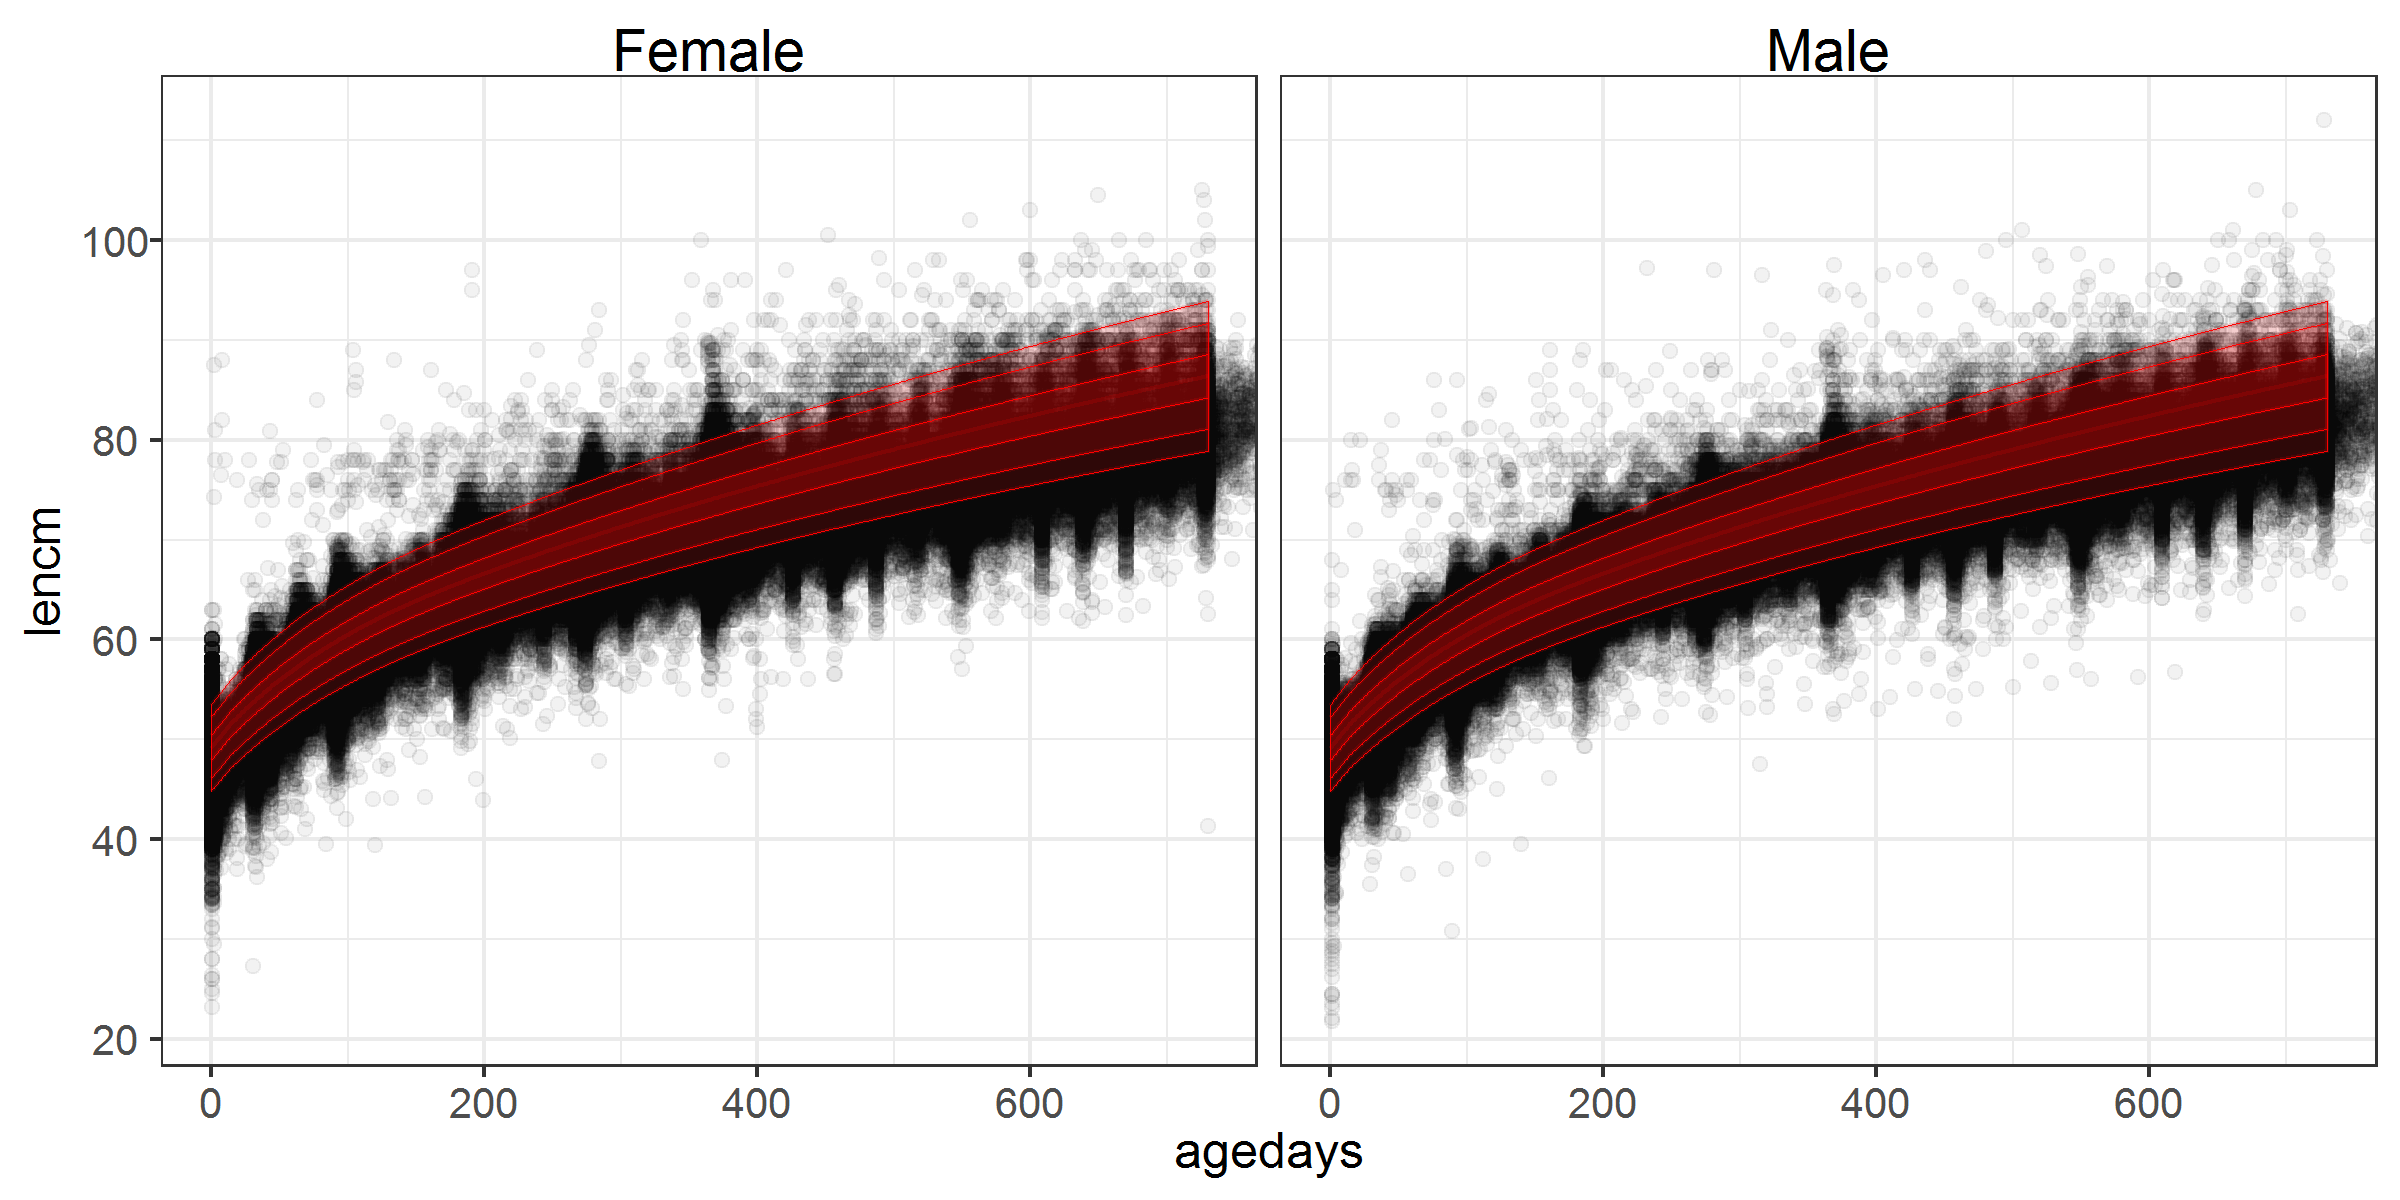
\includegraphics[width=33.33in]{C:/Users/andre/Documents/HBGDki/stunting/ki-longitudinal-manuscripts/figures/shared/laz_QA}

\includegraphics[width=104.17in]{C:/Users/andre/Documents/HBGDki/stunting/ki-longitudinal-manuscripts/figures/shared/laz_QA_cohort}

Revised files to be added - image was too large to push before

\chapter{Severe stunting analyses}\label{severe-stunting}

\raggedright

Below, we display plots for the age-specific prevalence and cumulative
incidence of severe stunting (LAZ \textless{} -3). Overall, the patterns
are the same as for stunting (LAZ \textless{} -2), with the peak in
prevalence at ages 18-24 months and the highest incidence proportion
from 0-3 months.

\section{Age-specific severe stunting
prevalence}\label{age-specific-severe-stunting-prevalence}

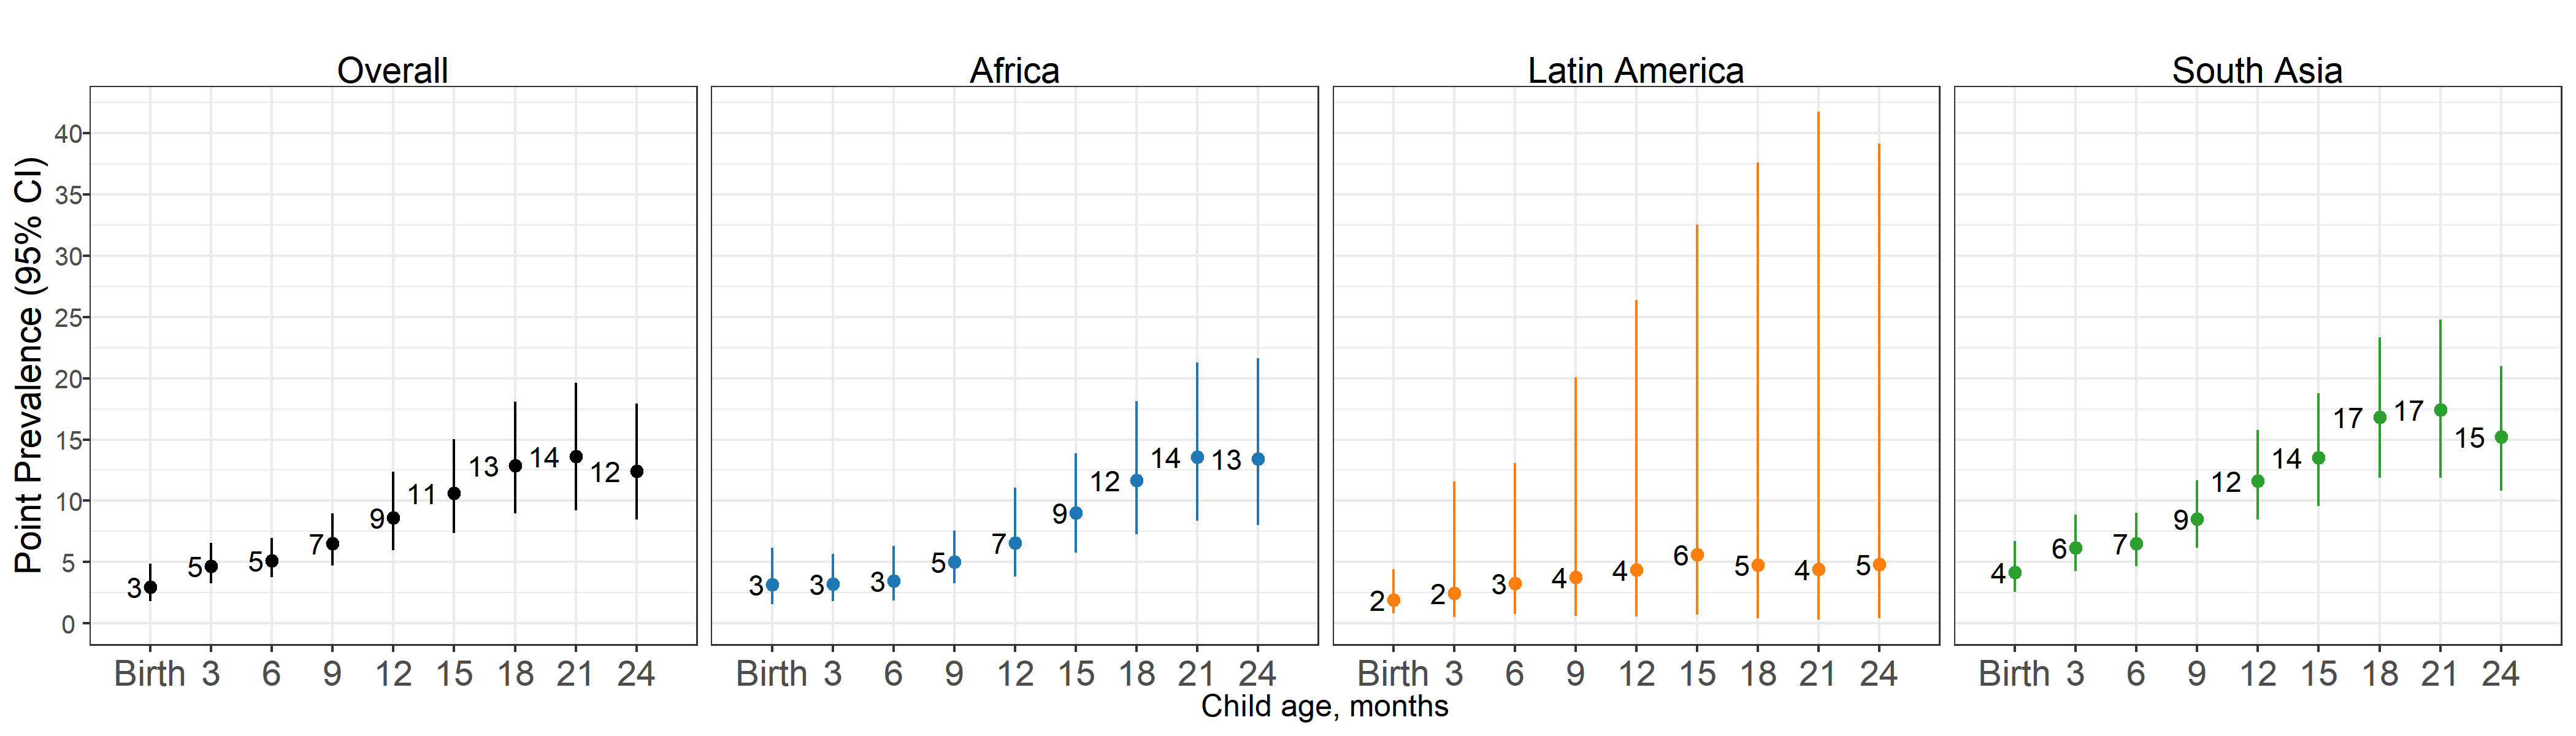
\includegraphics[width=58.33in]{C:/Users/andre/Documents/HBGDki/stunting/ki-longitudinal-manuscripts/figures/stunting/fig-stunt-3-prev-overall_region--allage-primary}

\section{Age-specific severe stunting
incidence}\label{age-specific-severe-stunting-incidence}

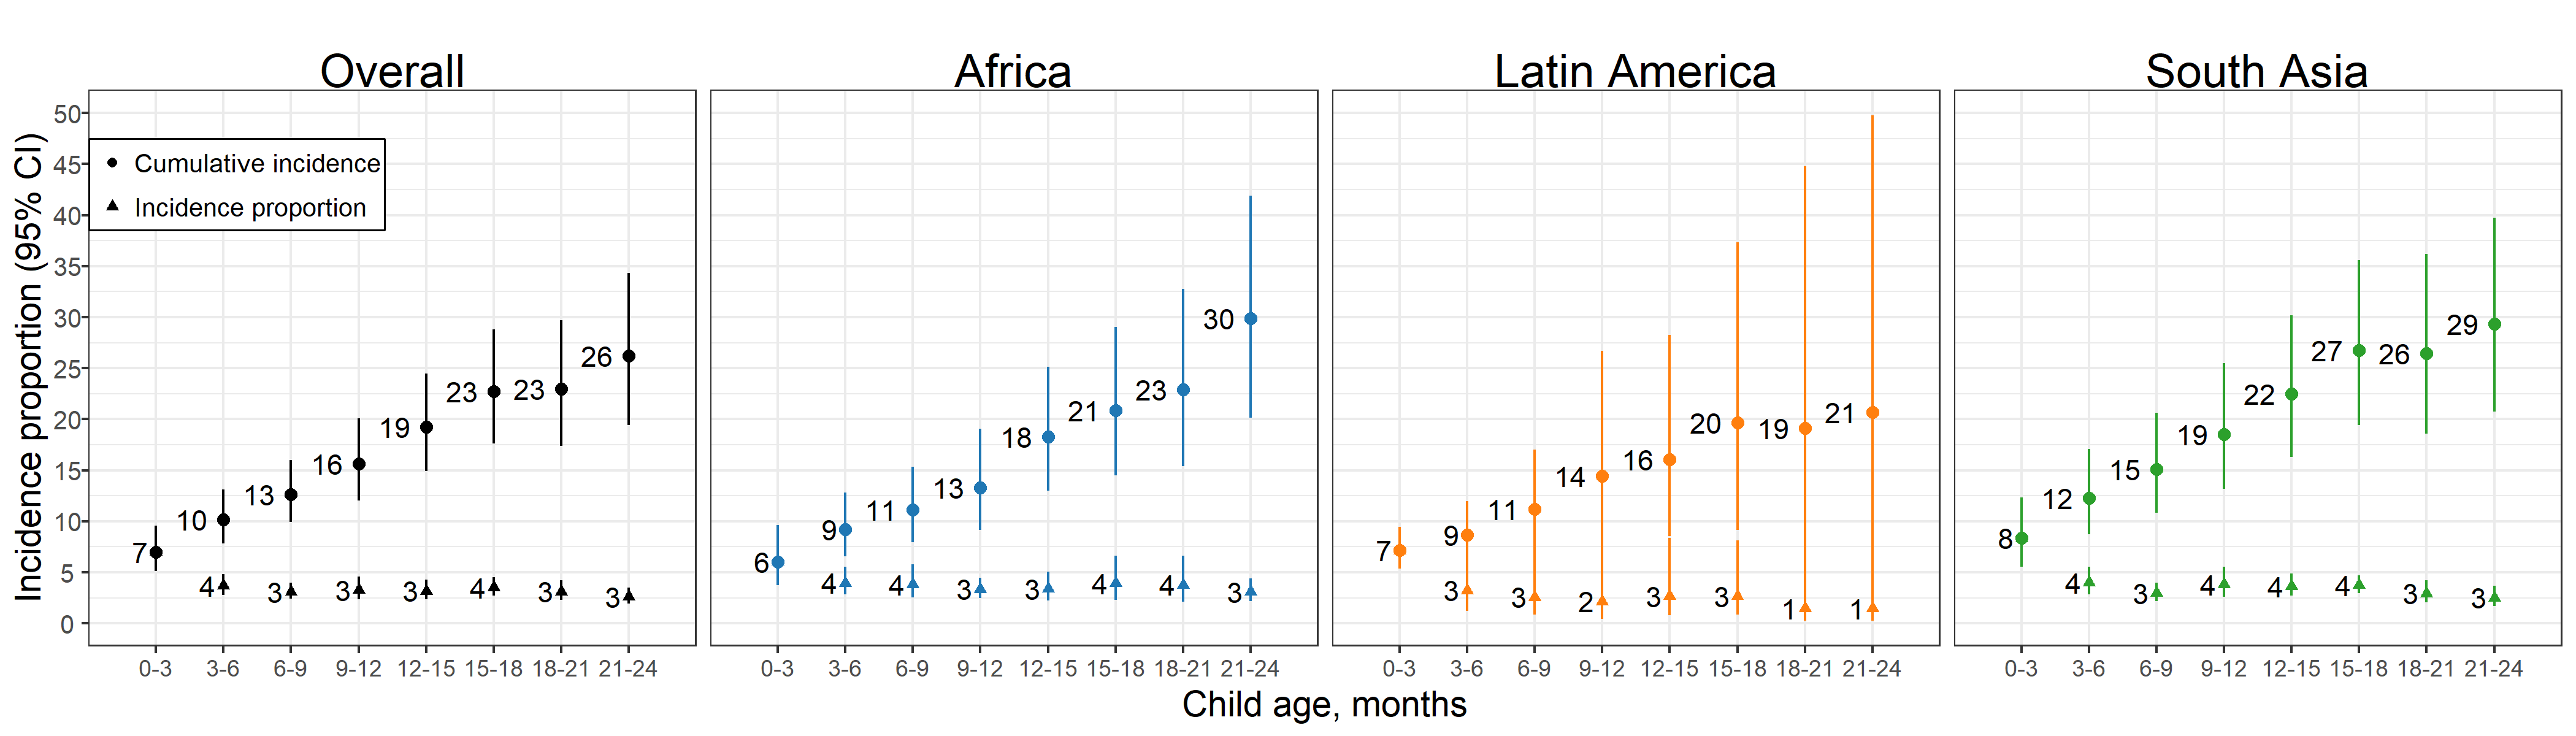
\includegraphics[width=58.33in]{C:/Users/andre/Documents/HBGDki/stunting/ki-longitudinal-manuscripts/figures/stunting/fig-stunt-3-inc-overall_region--allage-primary}

\chapter{Assessment of potential secular trends}\label{secular-trends}

\raggedright

This study included cohorts that measured child growth from 1969 to
2014. To assess potential secular trends, we plotted the mean
length-for-age Z-score (LAZ) over time. The plot below shows the
individual observations from included studies over this range of years.
There does not appear to be a secular trend in LAZ.

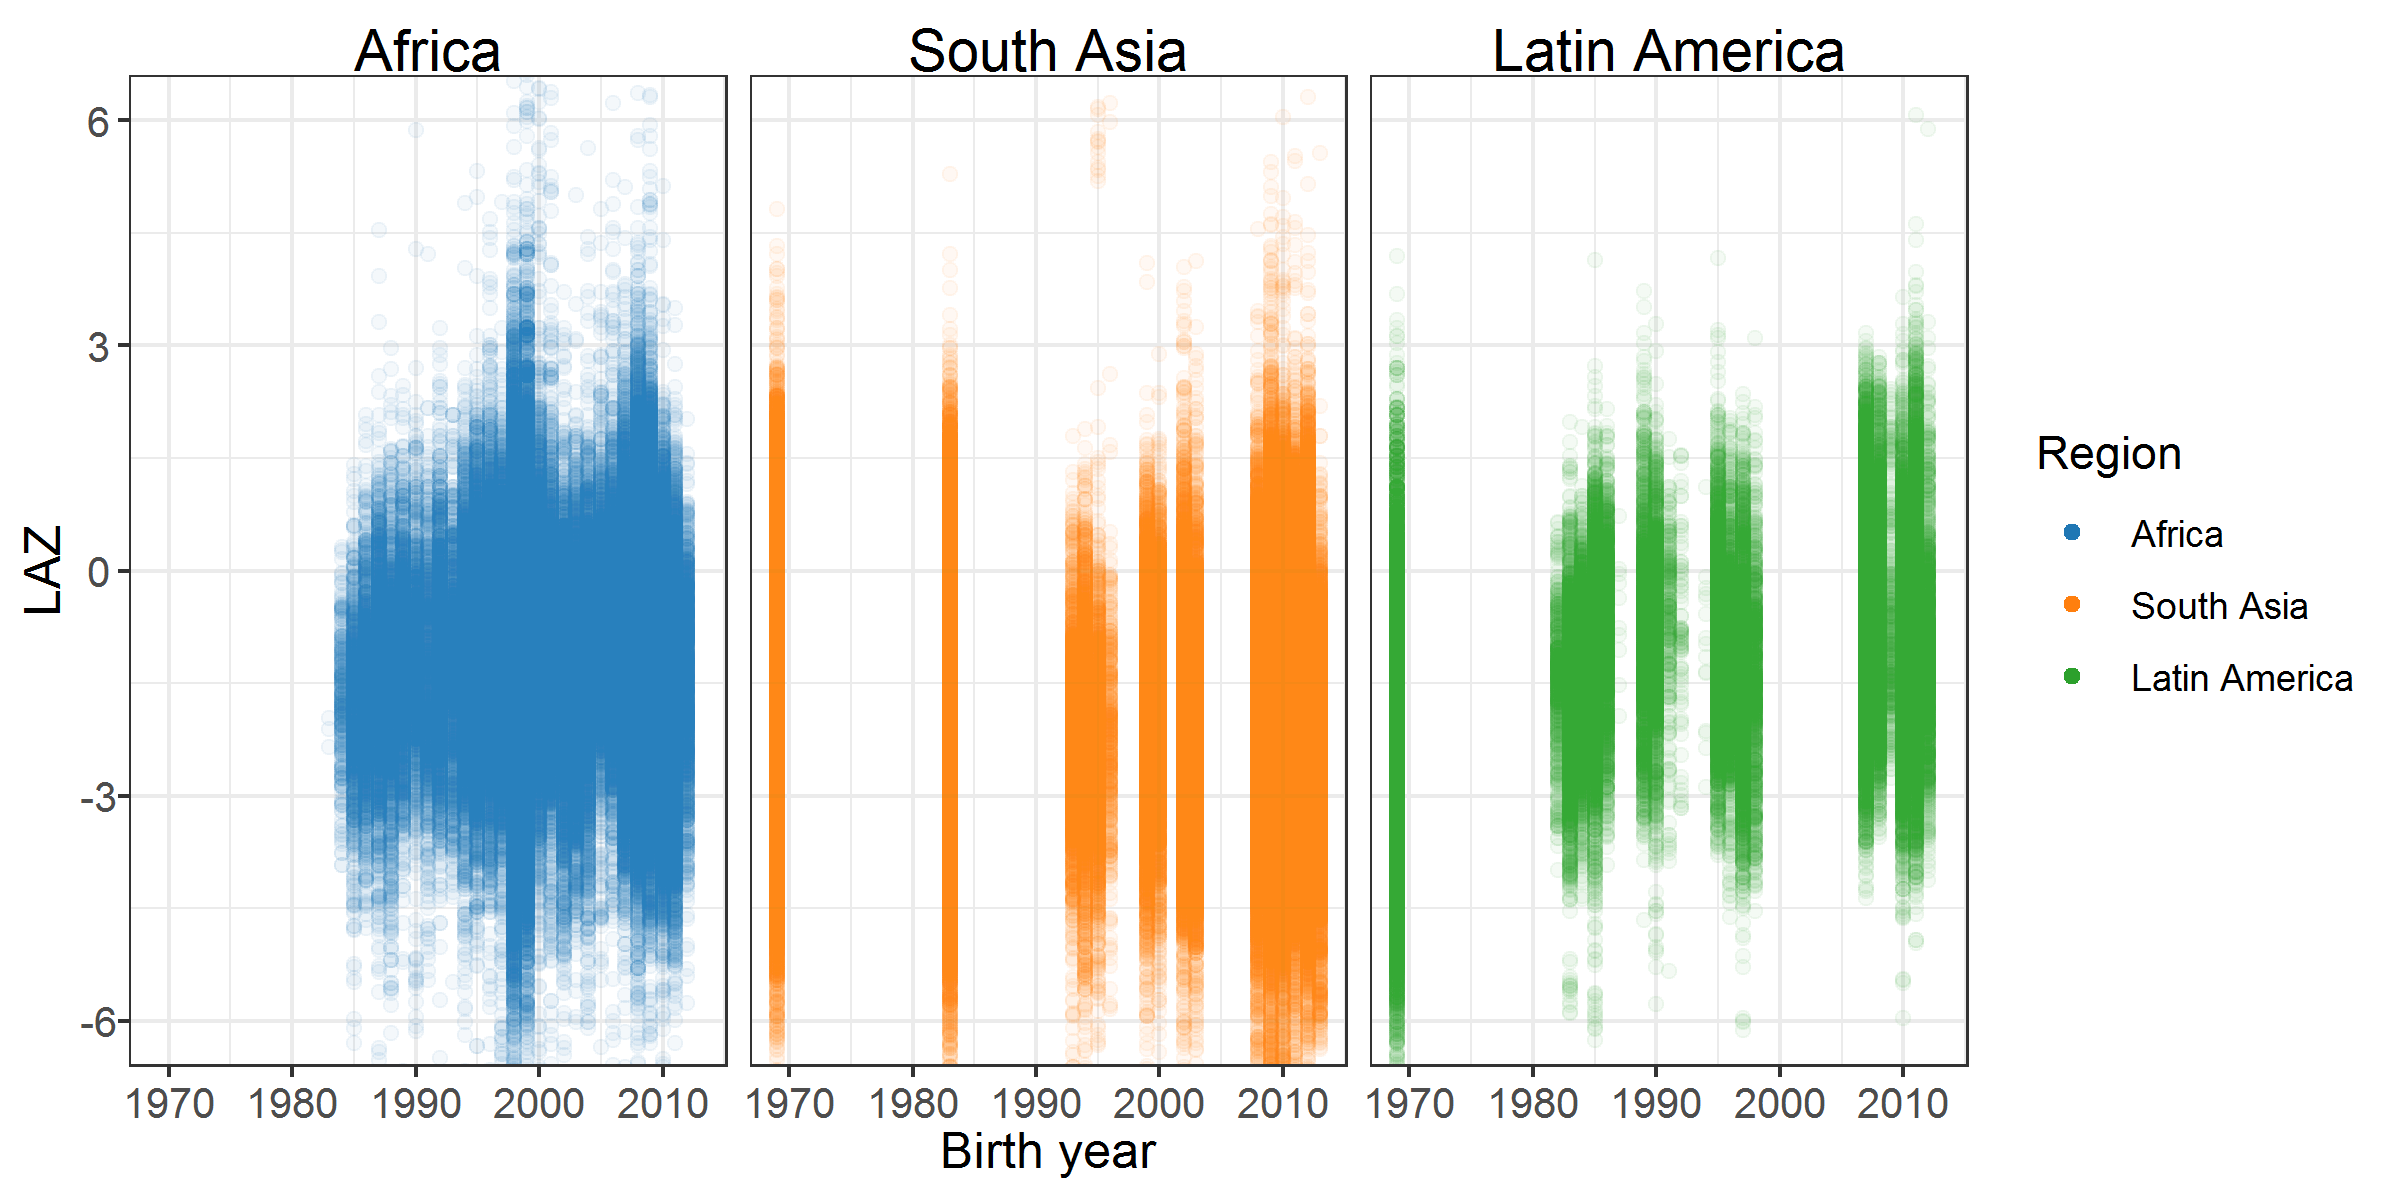
\includegraphics[width=33.33in]{C:/Users/andre/Documents/HBGDki/stunting/ki-longitudinal-manuscripts/figures/shared/laz_secular_trend}

\chapter{Analyses of age at first measurement}\label{age-meas}

\raggedright

Our analyses of stunting incidence assumed that children whose first
measurement occurred after birth were assumed to have experienced
stunting onset at the age halfway between birth and the first
measurement. To assess the extent to which this assumption influenced
our estimates, we plotted the distribution of age at first measurement
and the age at enrollment. The vast majority of children were enrolled
close to birth, and the majority were less than 5 days of age at their
first measurement.

\section{Histogram of first measurement within age 0-30
days}\label{histogram-of-first-measurement-within-age-0-30-days}

\subsection{All cohorts}\label{all-cohorts}

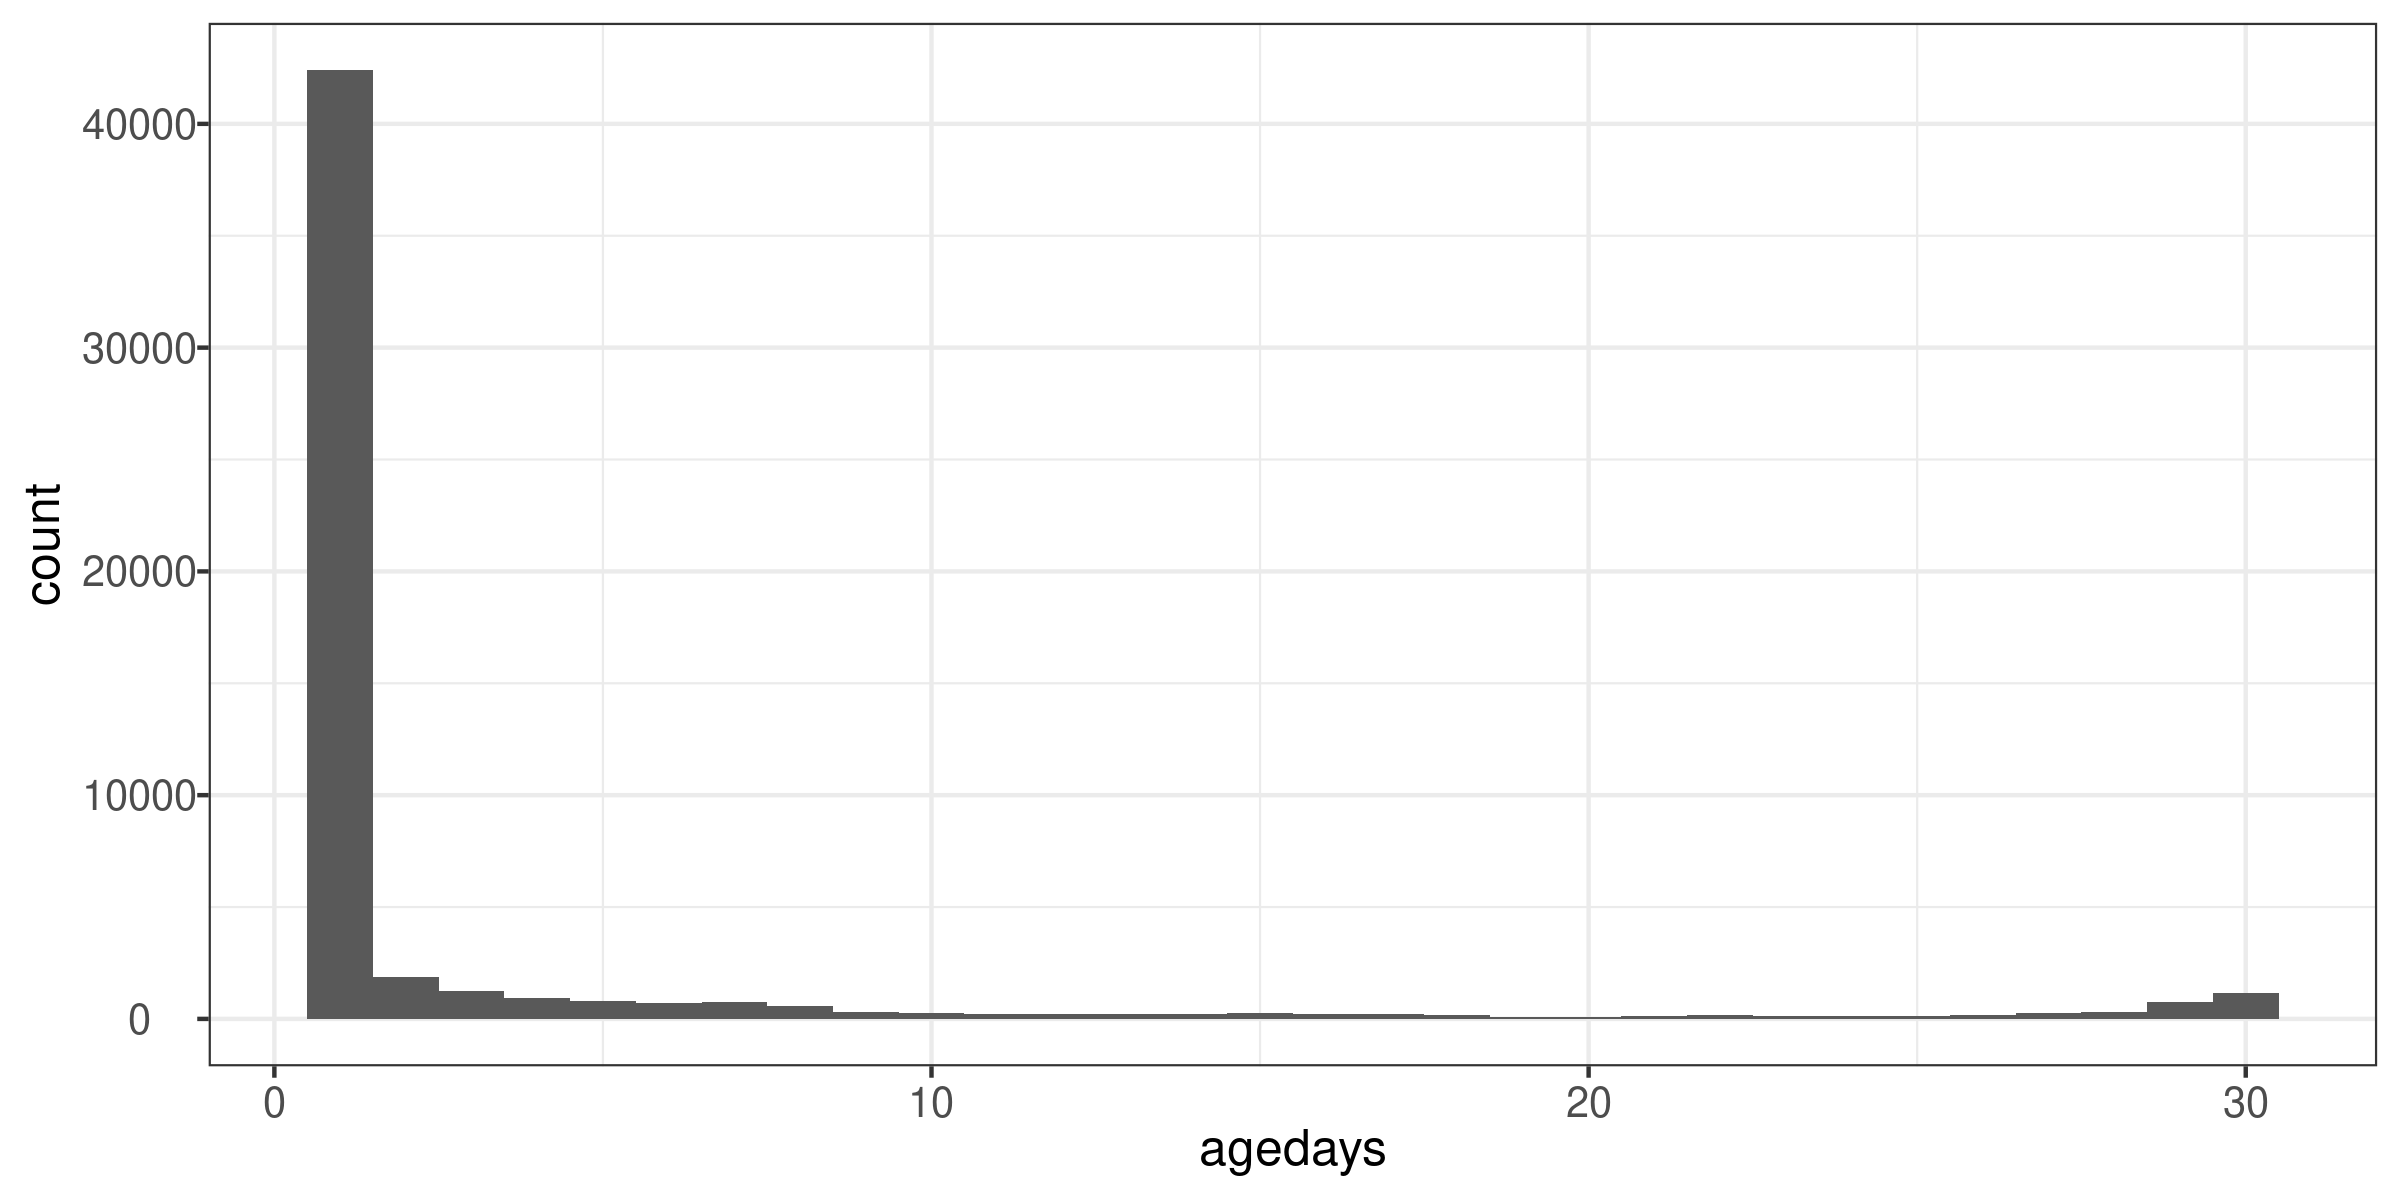
\includegraphics[width=33.33in]{C:/Users/andre/Documents/HBGDki/stunting/ki-longitudinal-manuscripts/figures/shared/age_histogram_first_month}

\subsection{Cohort-stratified}\label{cohort-stratified}

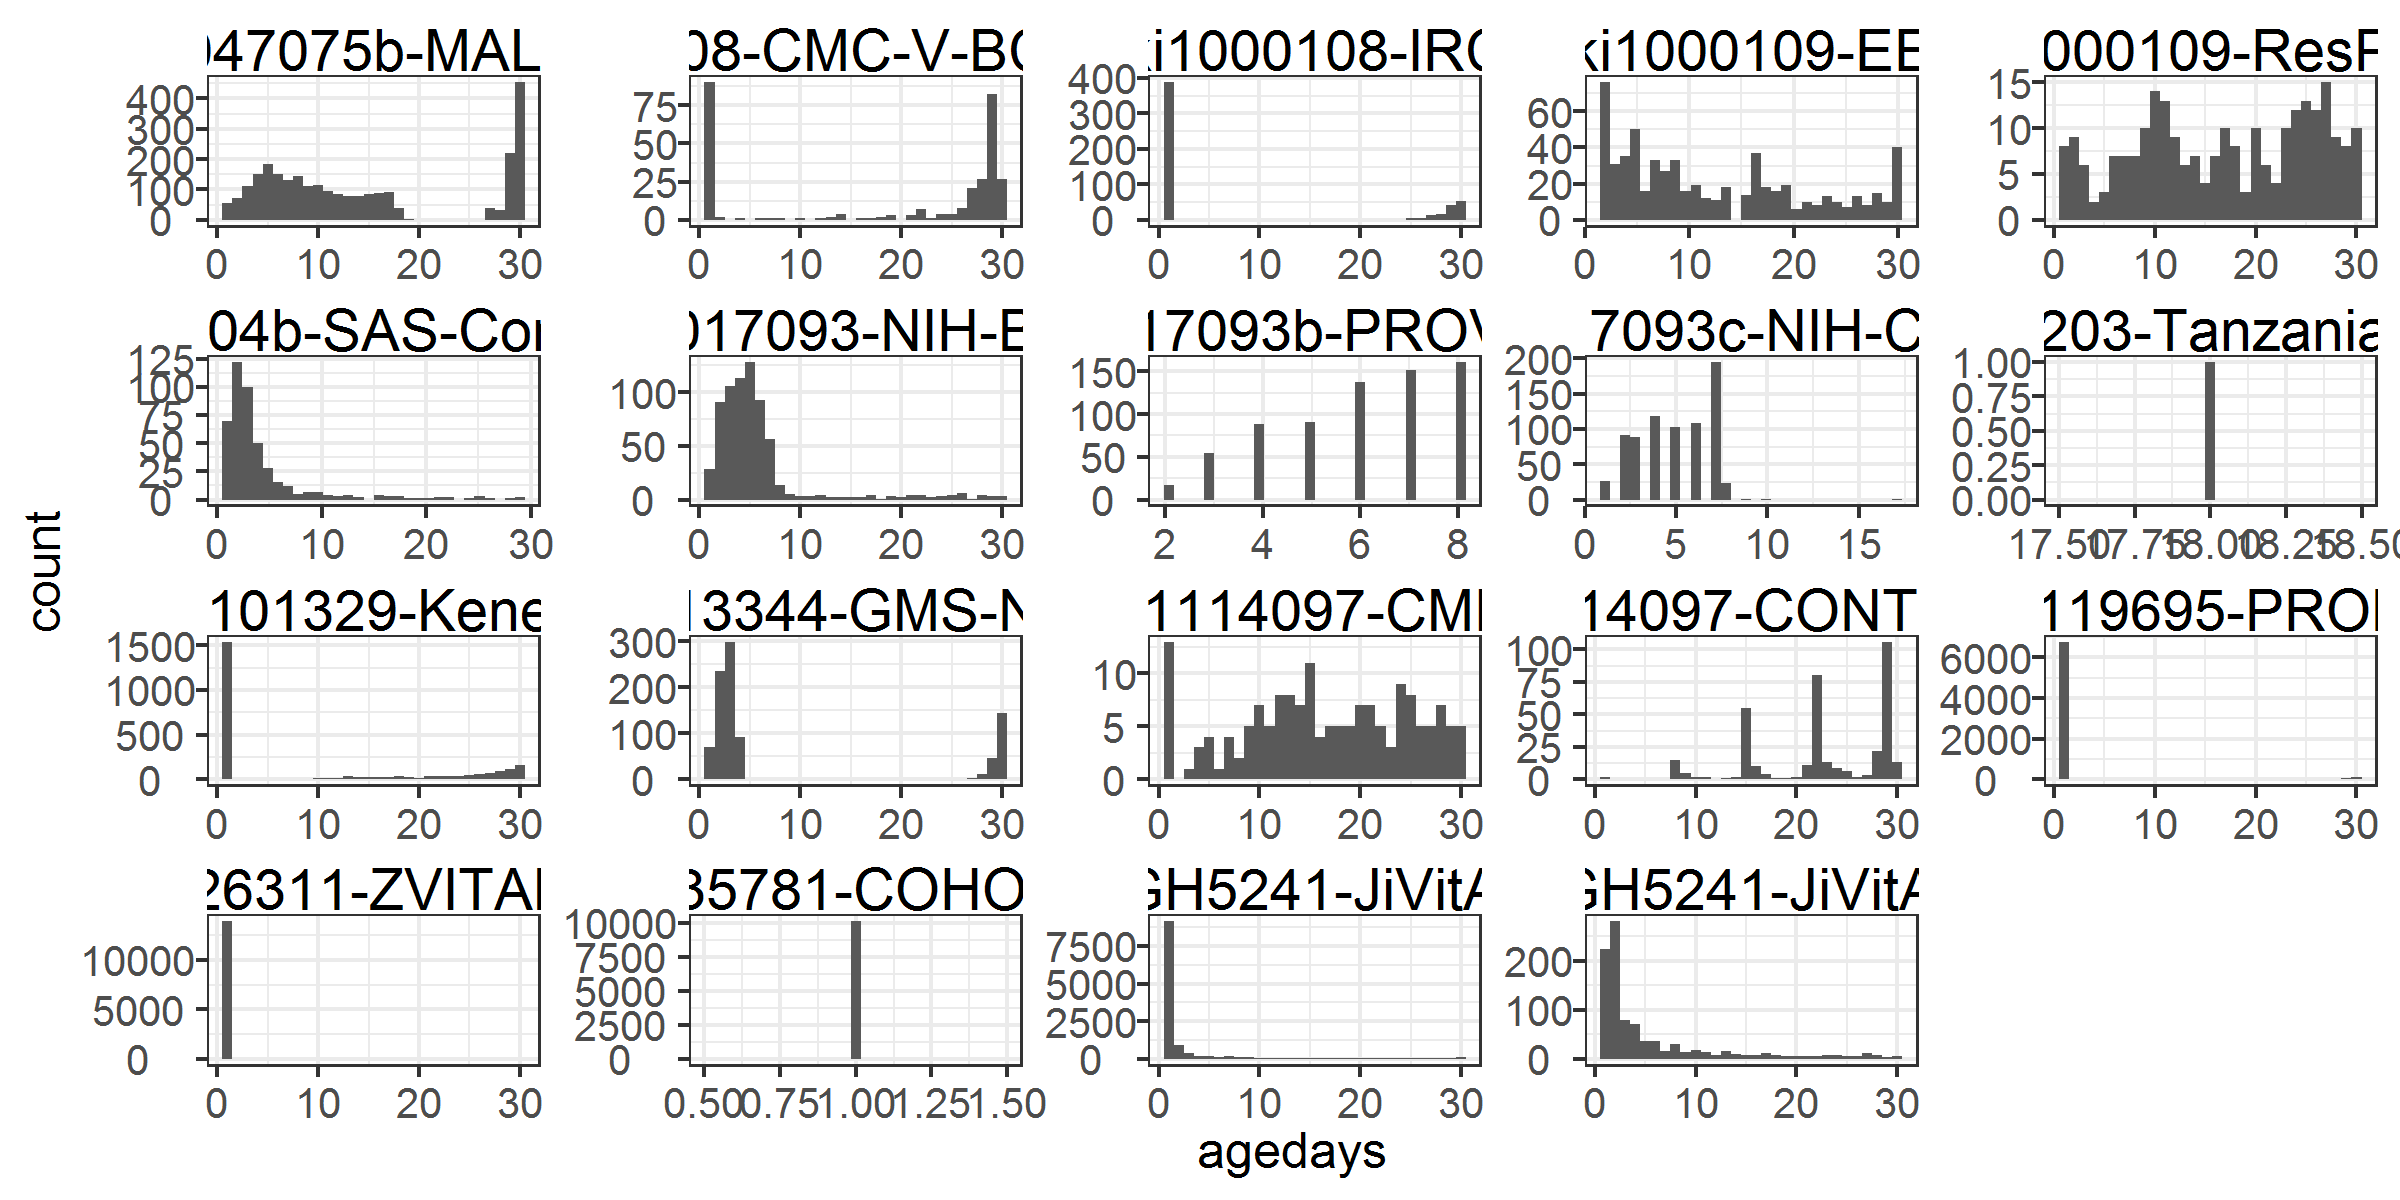
\includegraphics[width=33.33in]{C:/Users/andre/Documents/HBGDki/stunting/ki-longitudinal-manuscripts/figures/shared/age_histogram_first_month_cohort}

\section{Histogram of age at
enrollment}\label{histogram-of-age-at-enrollment}

\subsection{All cohorts}\label{all-cohorts-1}

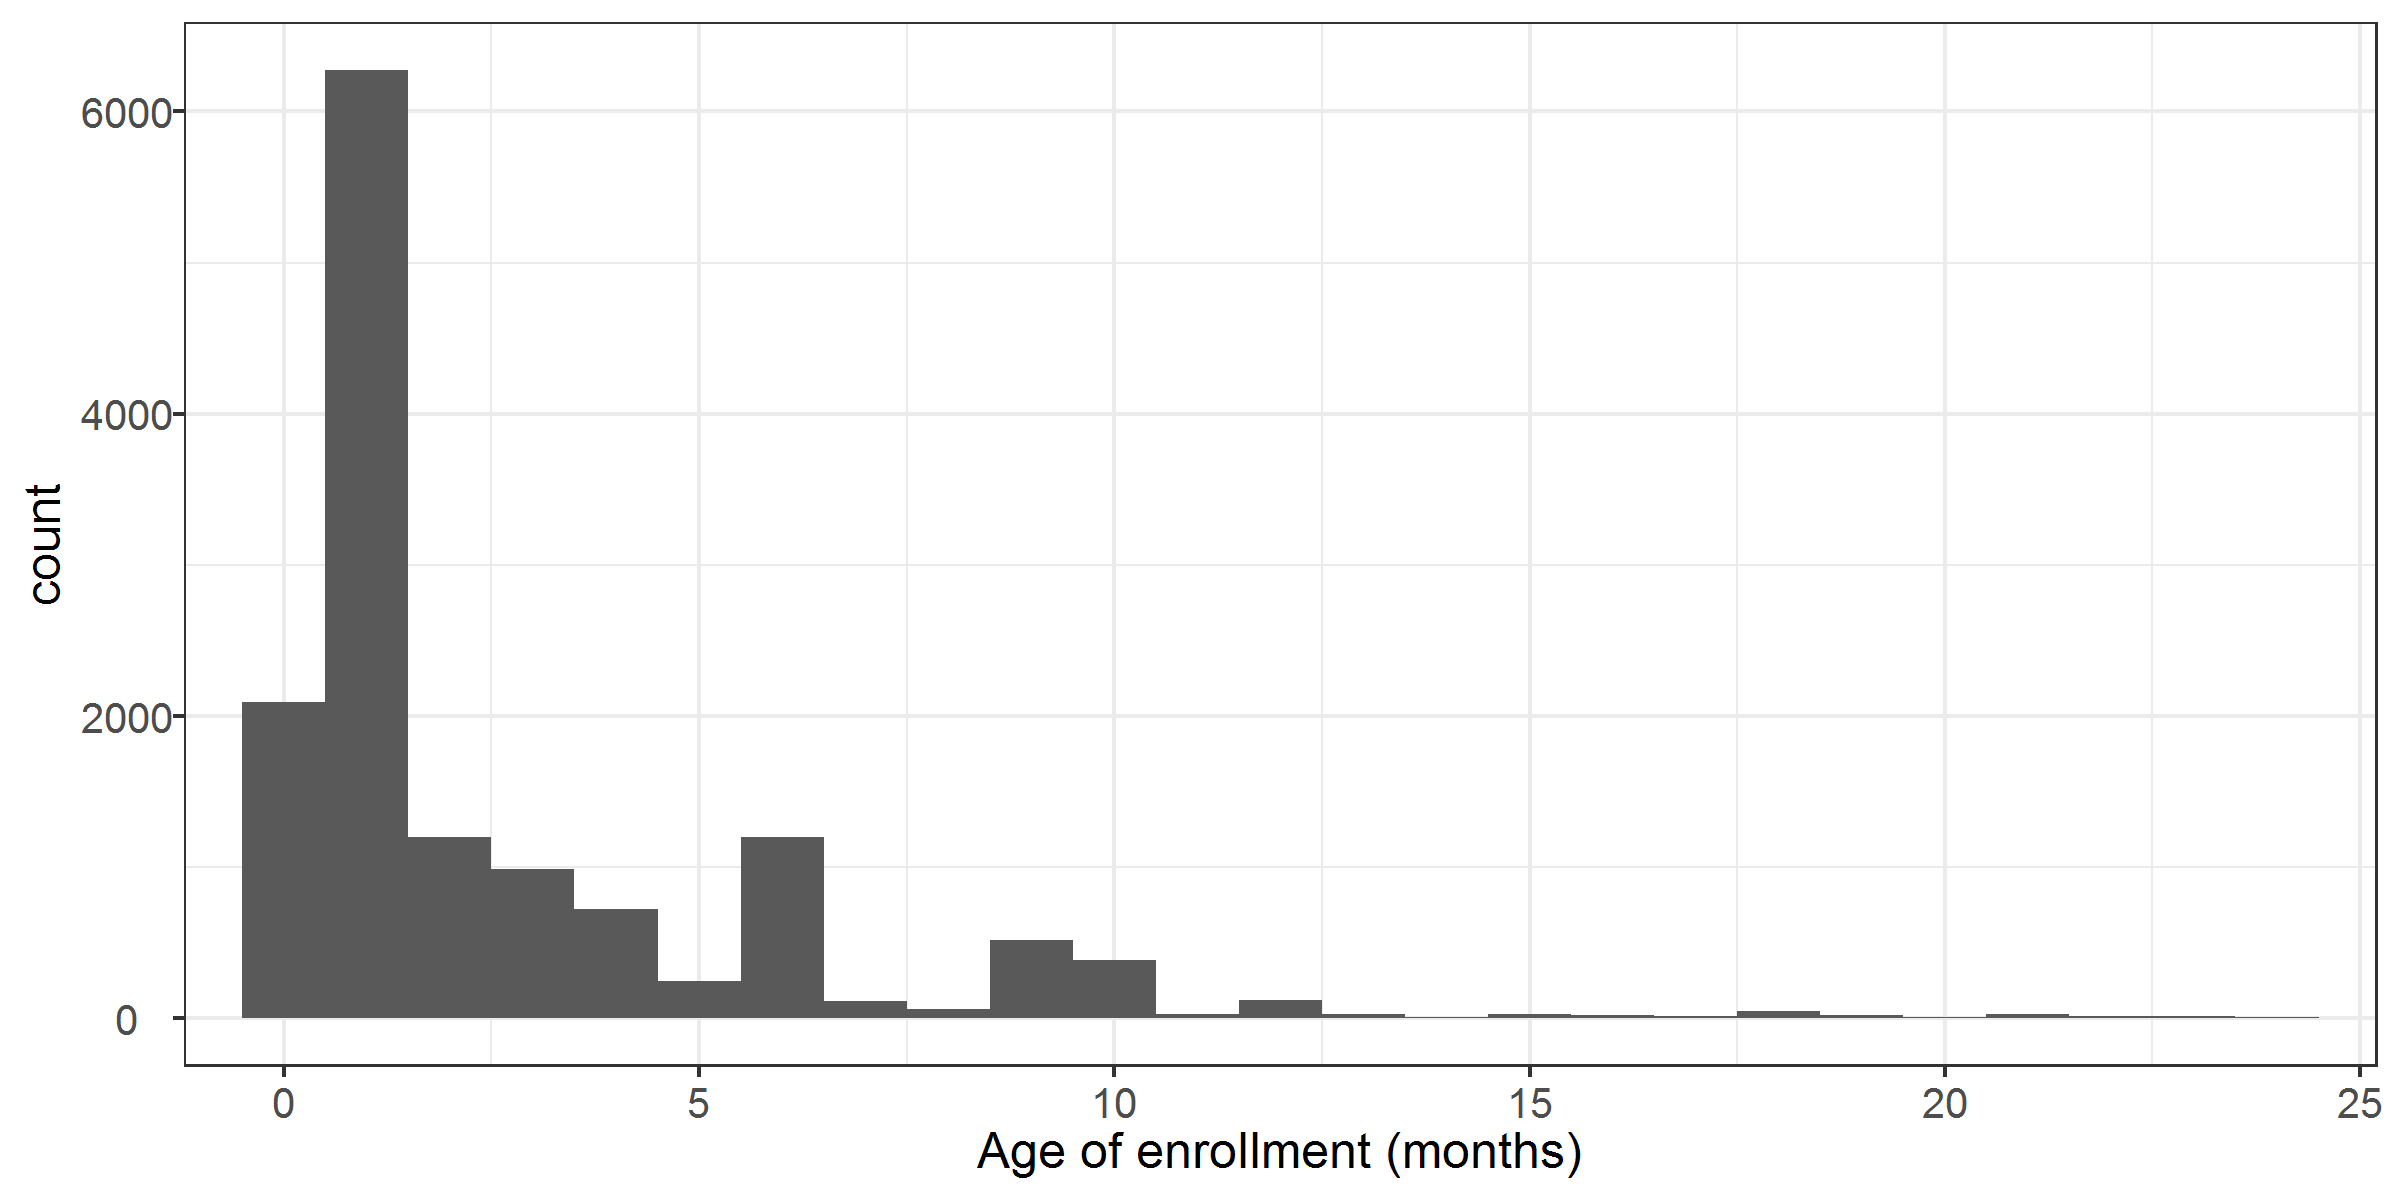
\includegraphics[width=33.33in]{C:/Users/andre/Documents/HBGDki/stunting/ki-longitudinal-manuscripts/figures/shared/enrollment_age_histogram_over_7d}

\subsection{Cohort-stratified}\label{cohort-stratified-1}

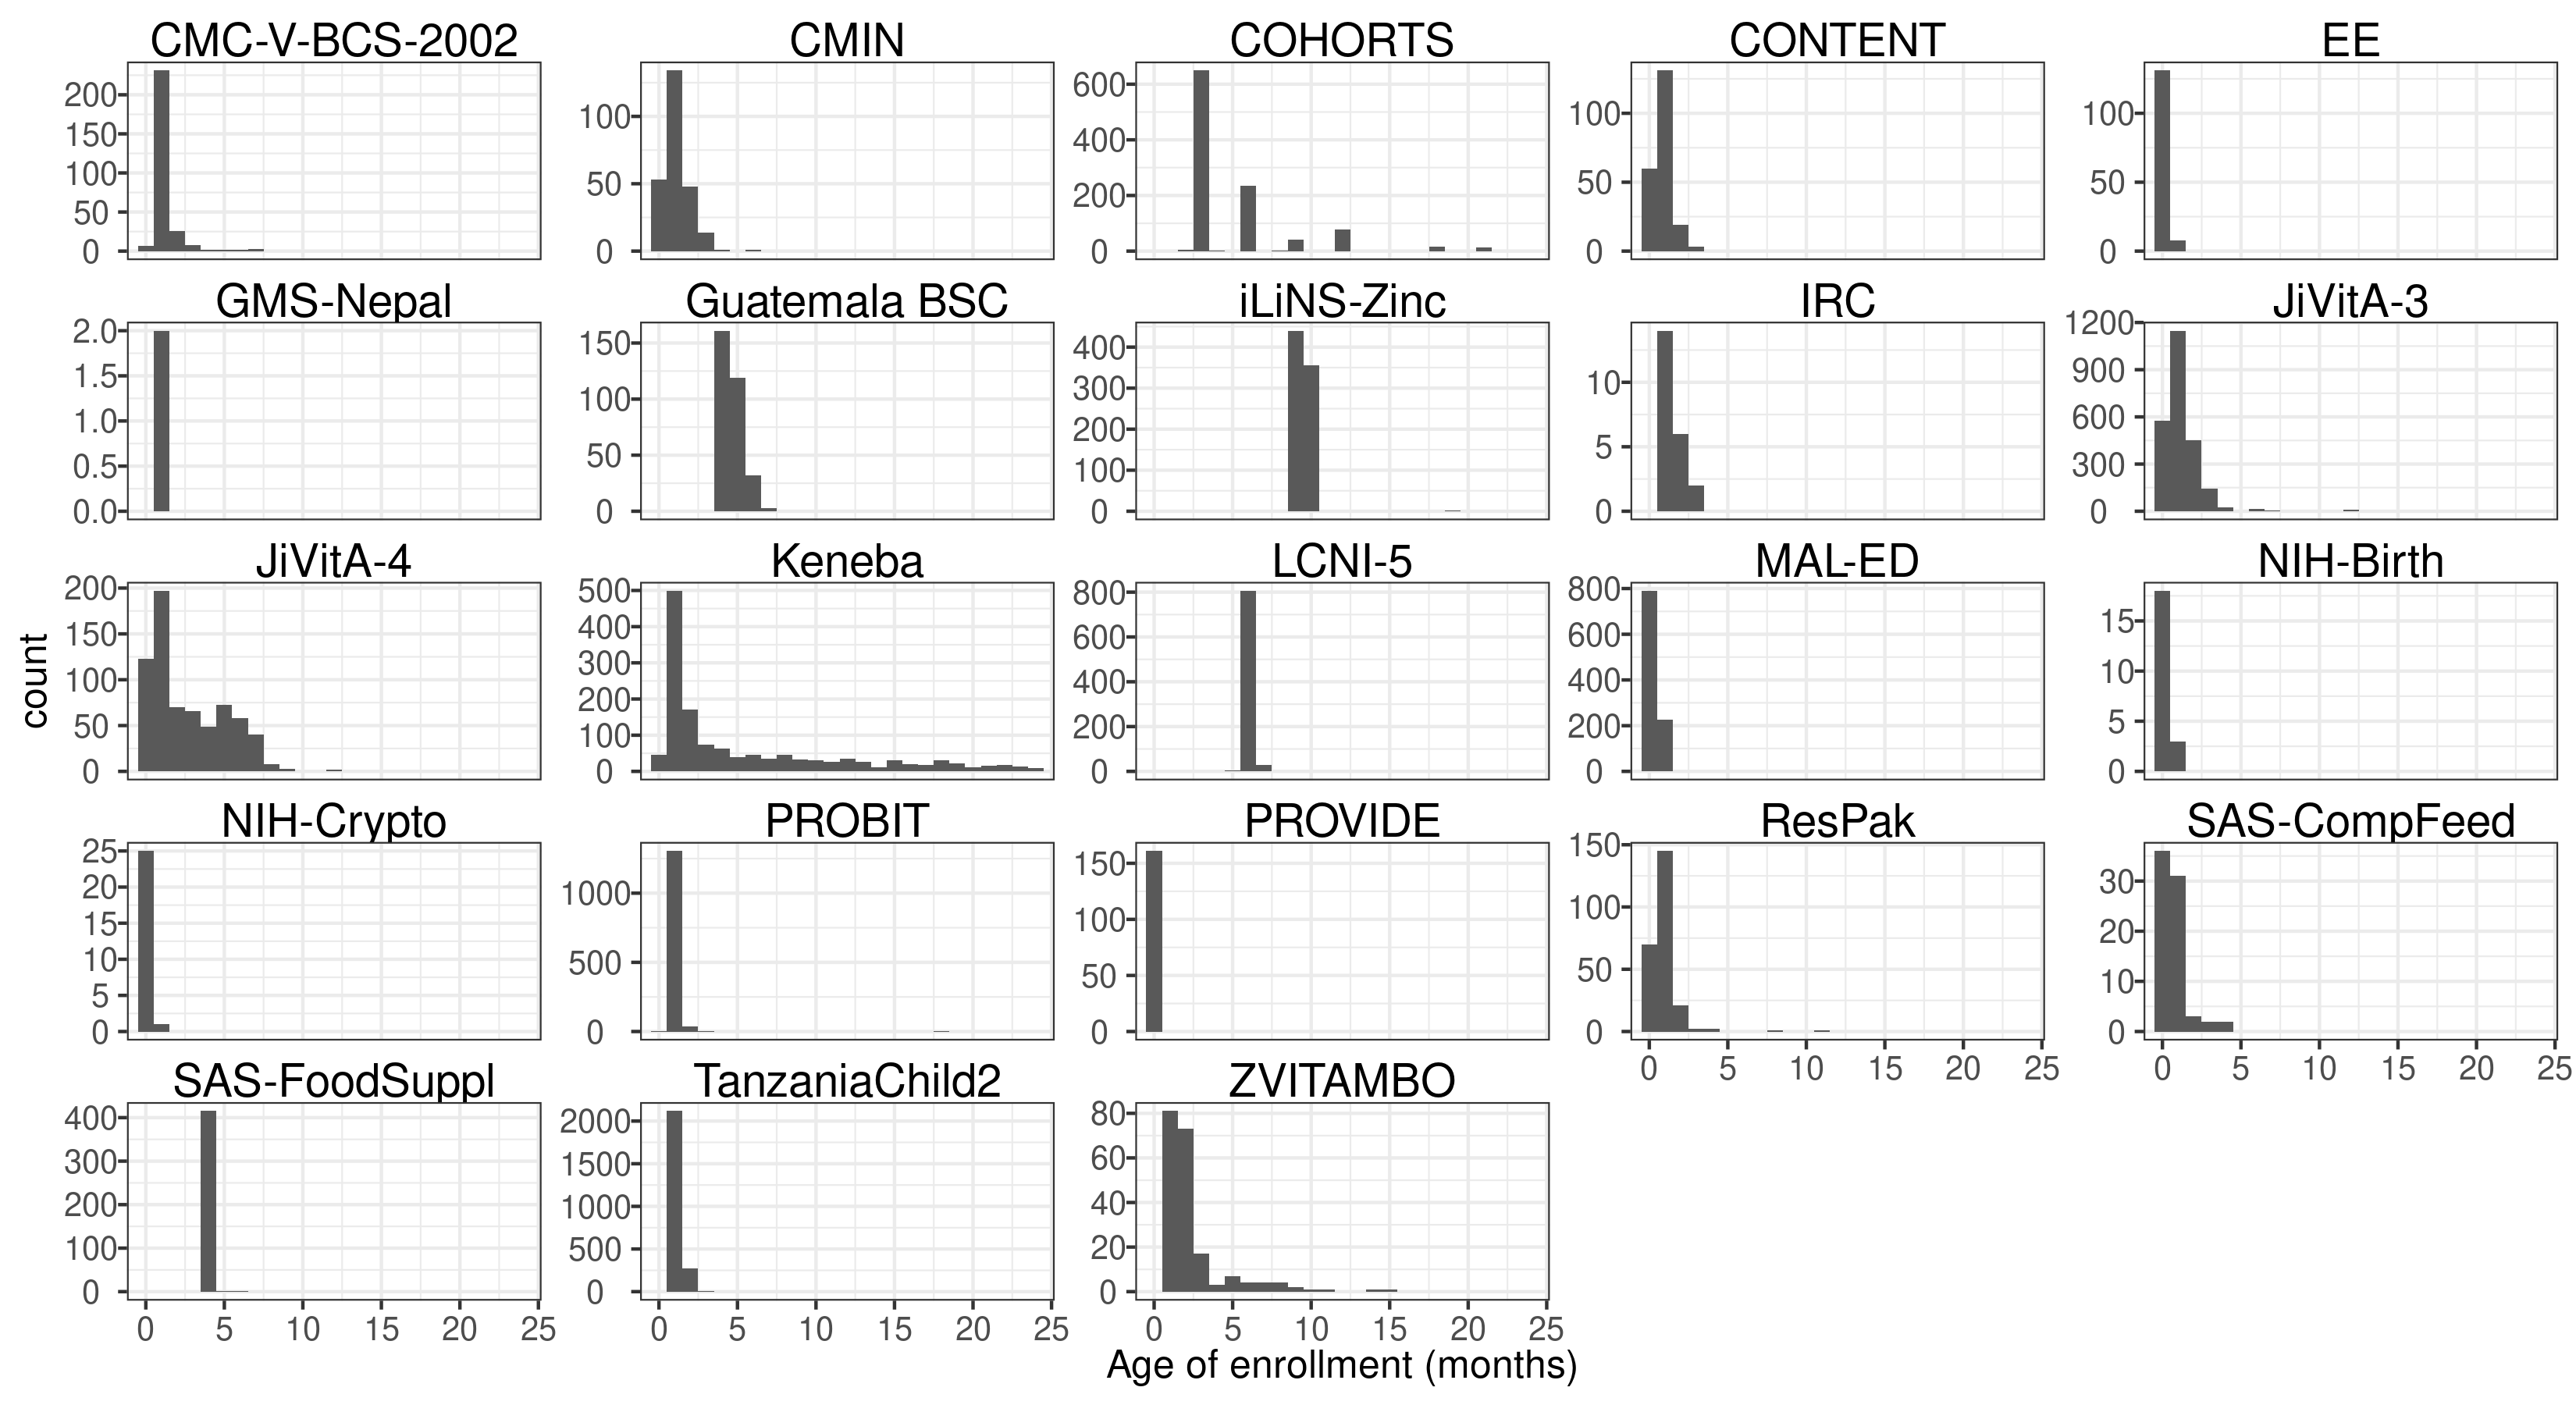
\includegraphics[width=33.33in]{C:/Users/andre/Documents/HBGDki/stunting/ki-longitudinal-manuscripts/figures/shared/enrollment_age_histogram_over_7d_cohort}

\chapter{Comparison to DHS surveys from matching countries}\label{DHS}

\raggedright

In the manuscript, we compared the mean length-for-age Z-score by age
and region in our included studies and in Demographic and Health Survey
(DHS) datasets from the same countries as those included in our study.
Here we present analogous plots including all of the countries from each
region. {[}add details interpreting figure{]}

{[}Figure to be added{]}

\chapter{Cohort-specific results}\label{cohort}

\raggedright

Here, we present cohort-specific estimates of length-for-age Z-score by
age, age-specific prevalence, and age-specific incidence.

\section{Mean length-for-age Z-score by
age}\label{mean-length-for-age-z-score-by-age}

\subsection{Africa}\label{africa}

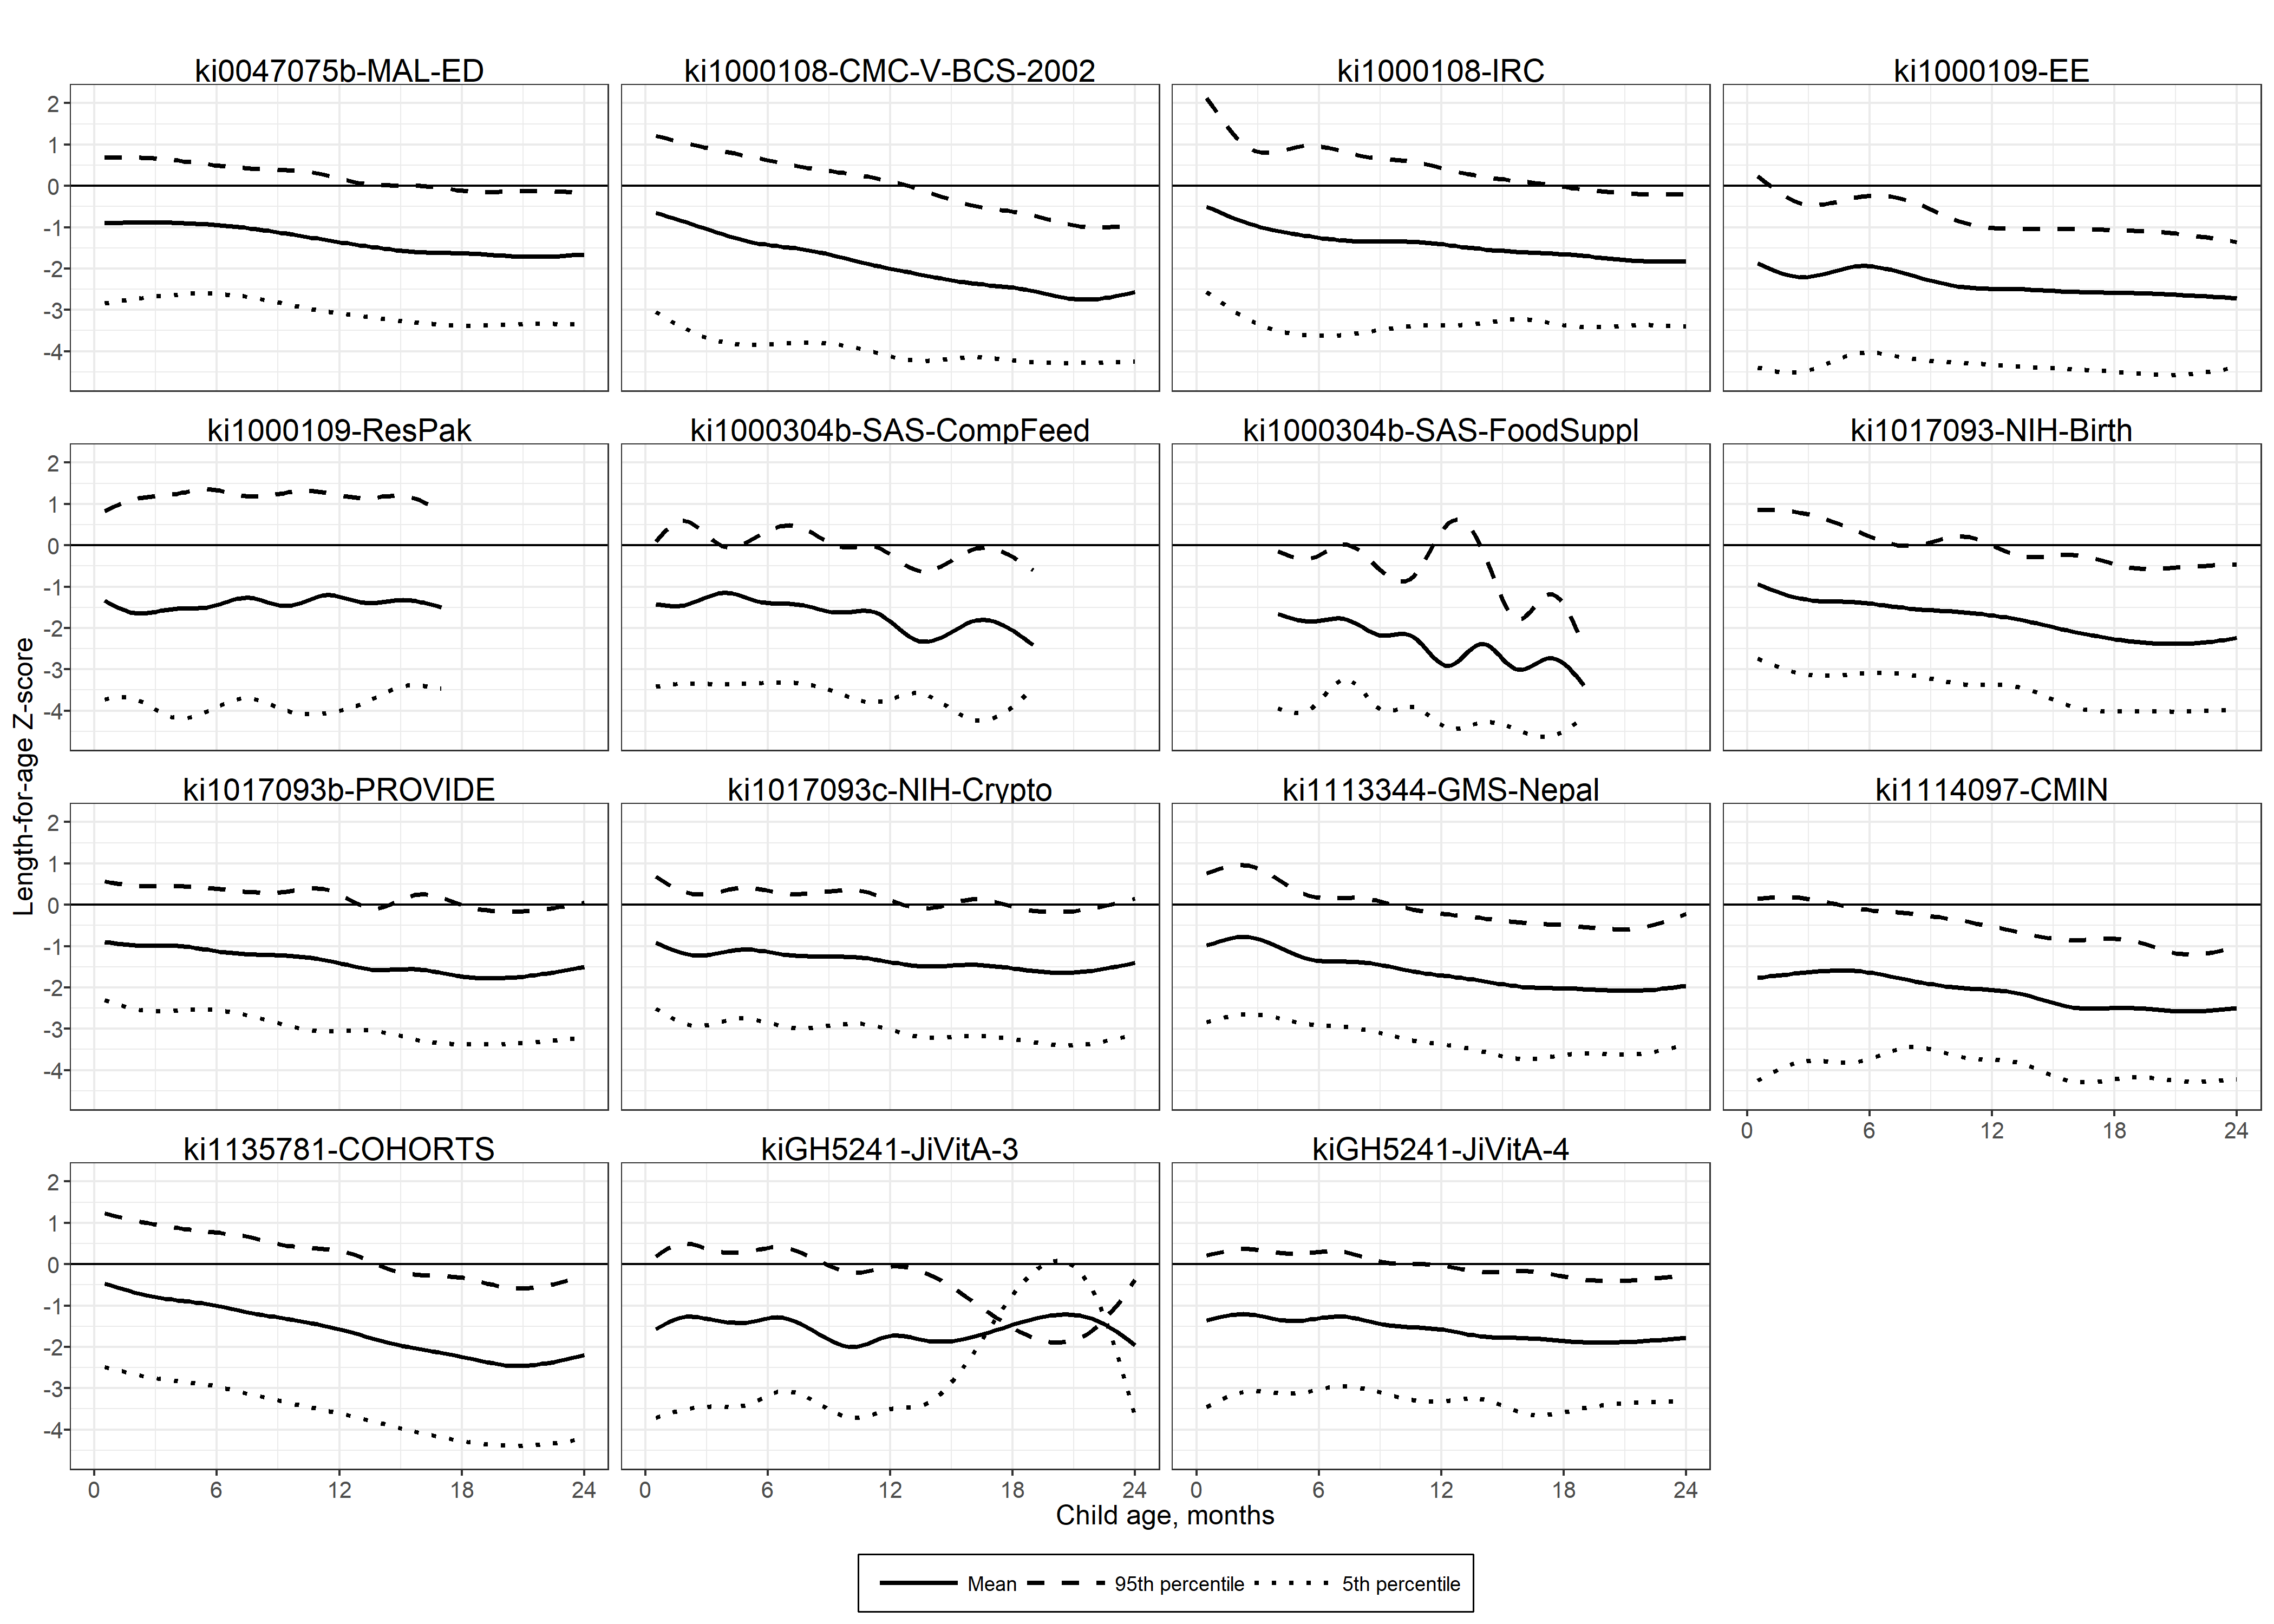
\includegraphics[width=58.33in]{C:/Users/andre/Documents/HBGDki/stunting/ki-longitudinal-manuscripts/figures/stunting/fig-laz-2-quant-cohort-africa-allage-primary}

\subsection{Latin America}\label{latin-america}

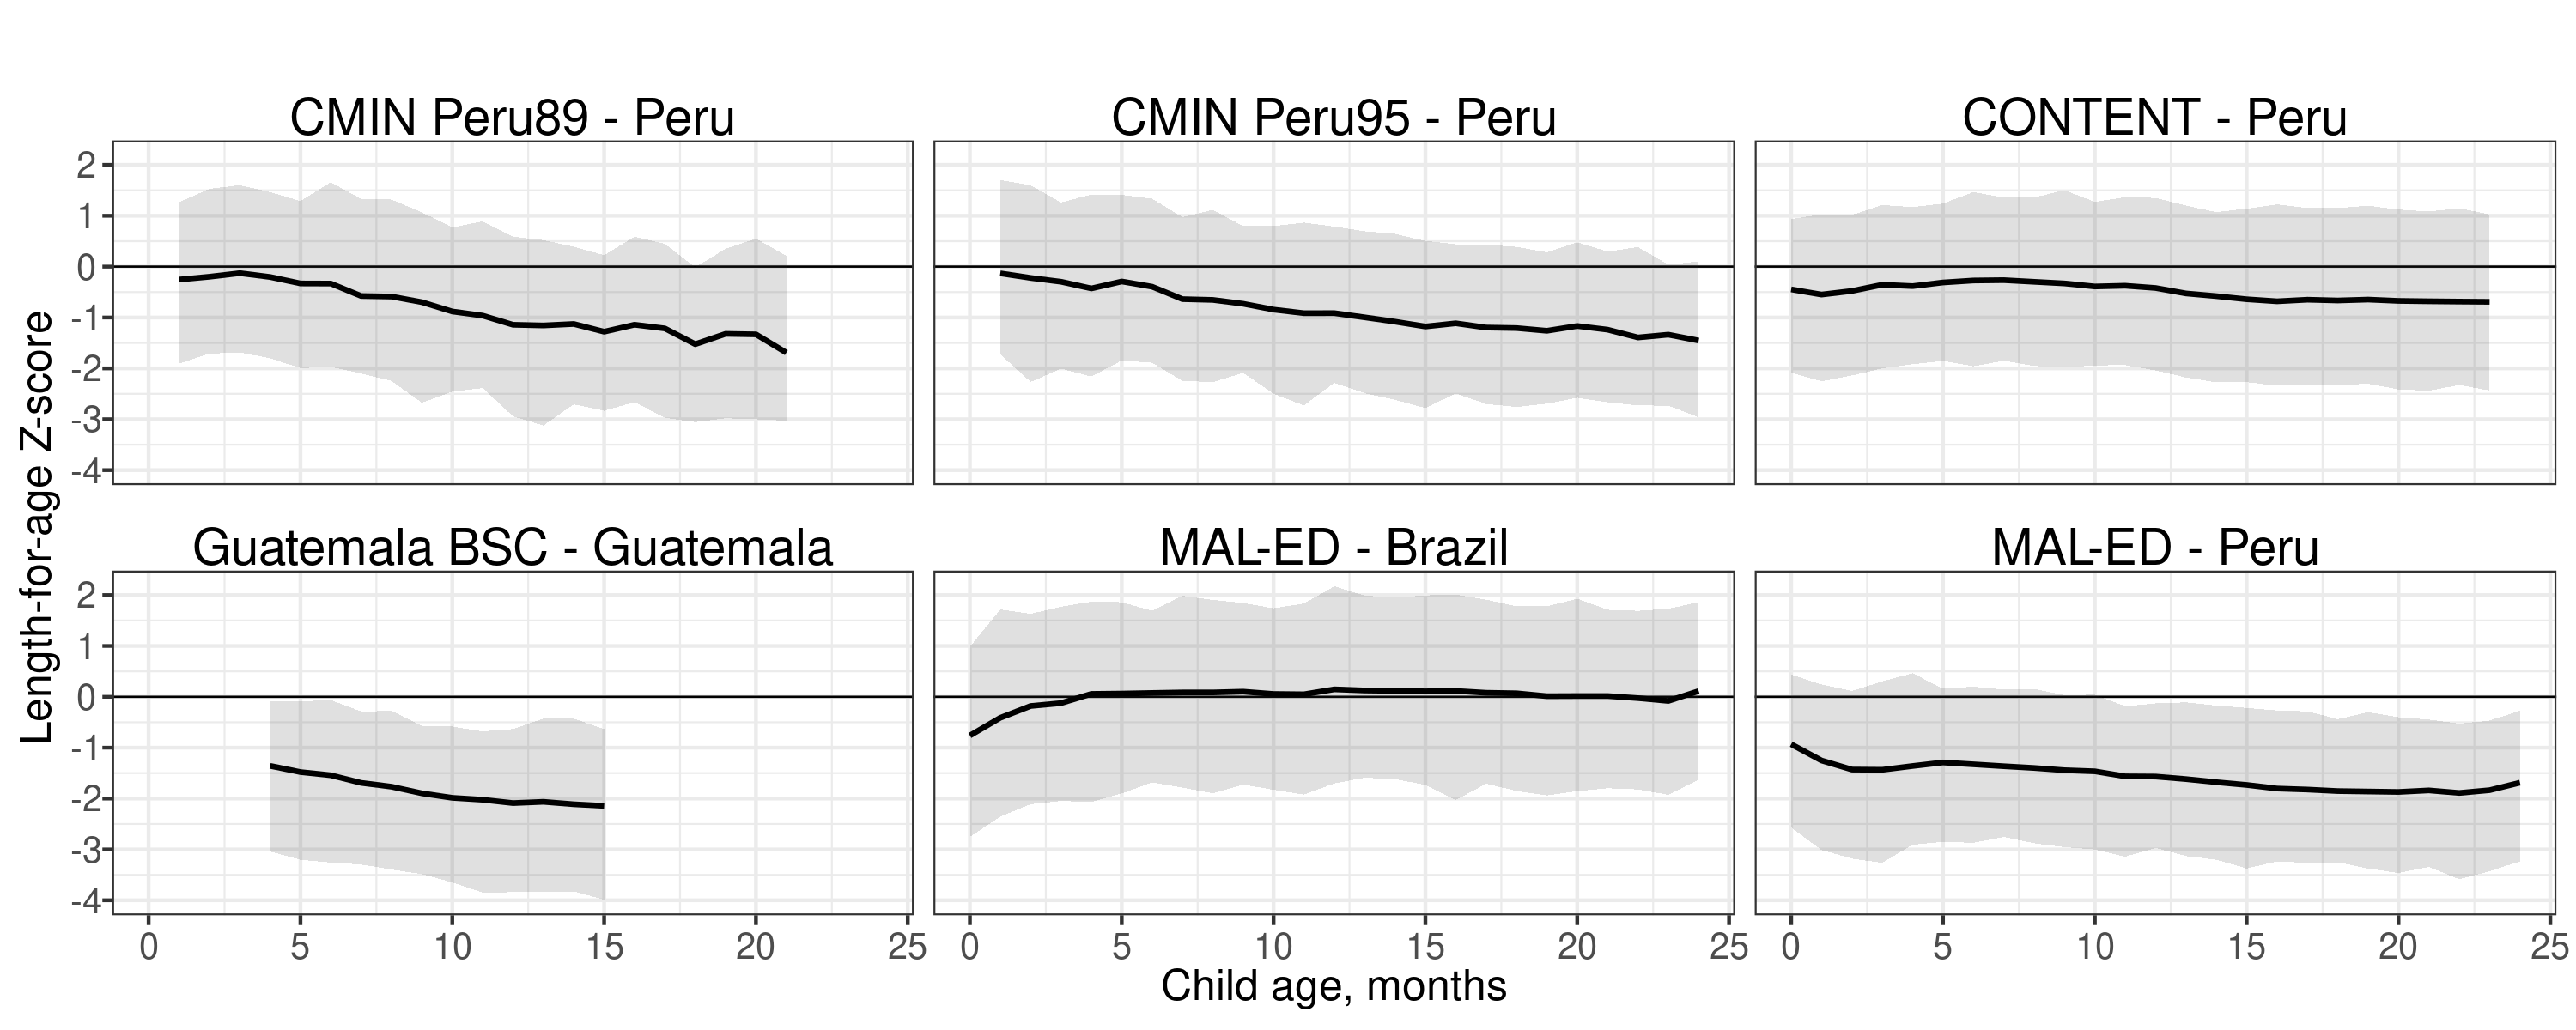
\includegraphics[width=58.33in]{C:/Users/andre/Documents/HBGDki/stunting/ki-longitudinal-manuscripts/figures/stunting/fig-laz-2-quant-cohort-latamer-allage-primary}

\subsection{South Asia}\label{south-asia}

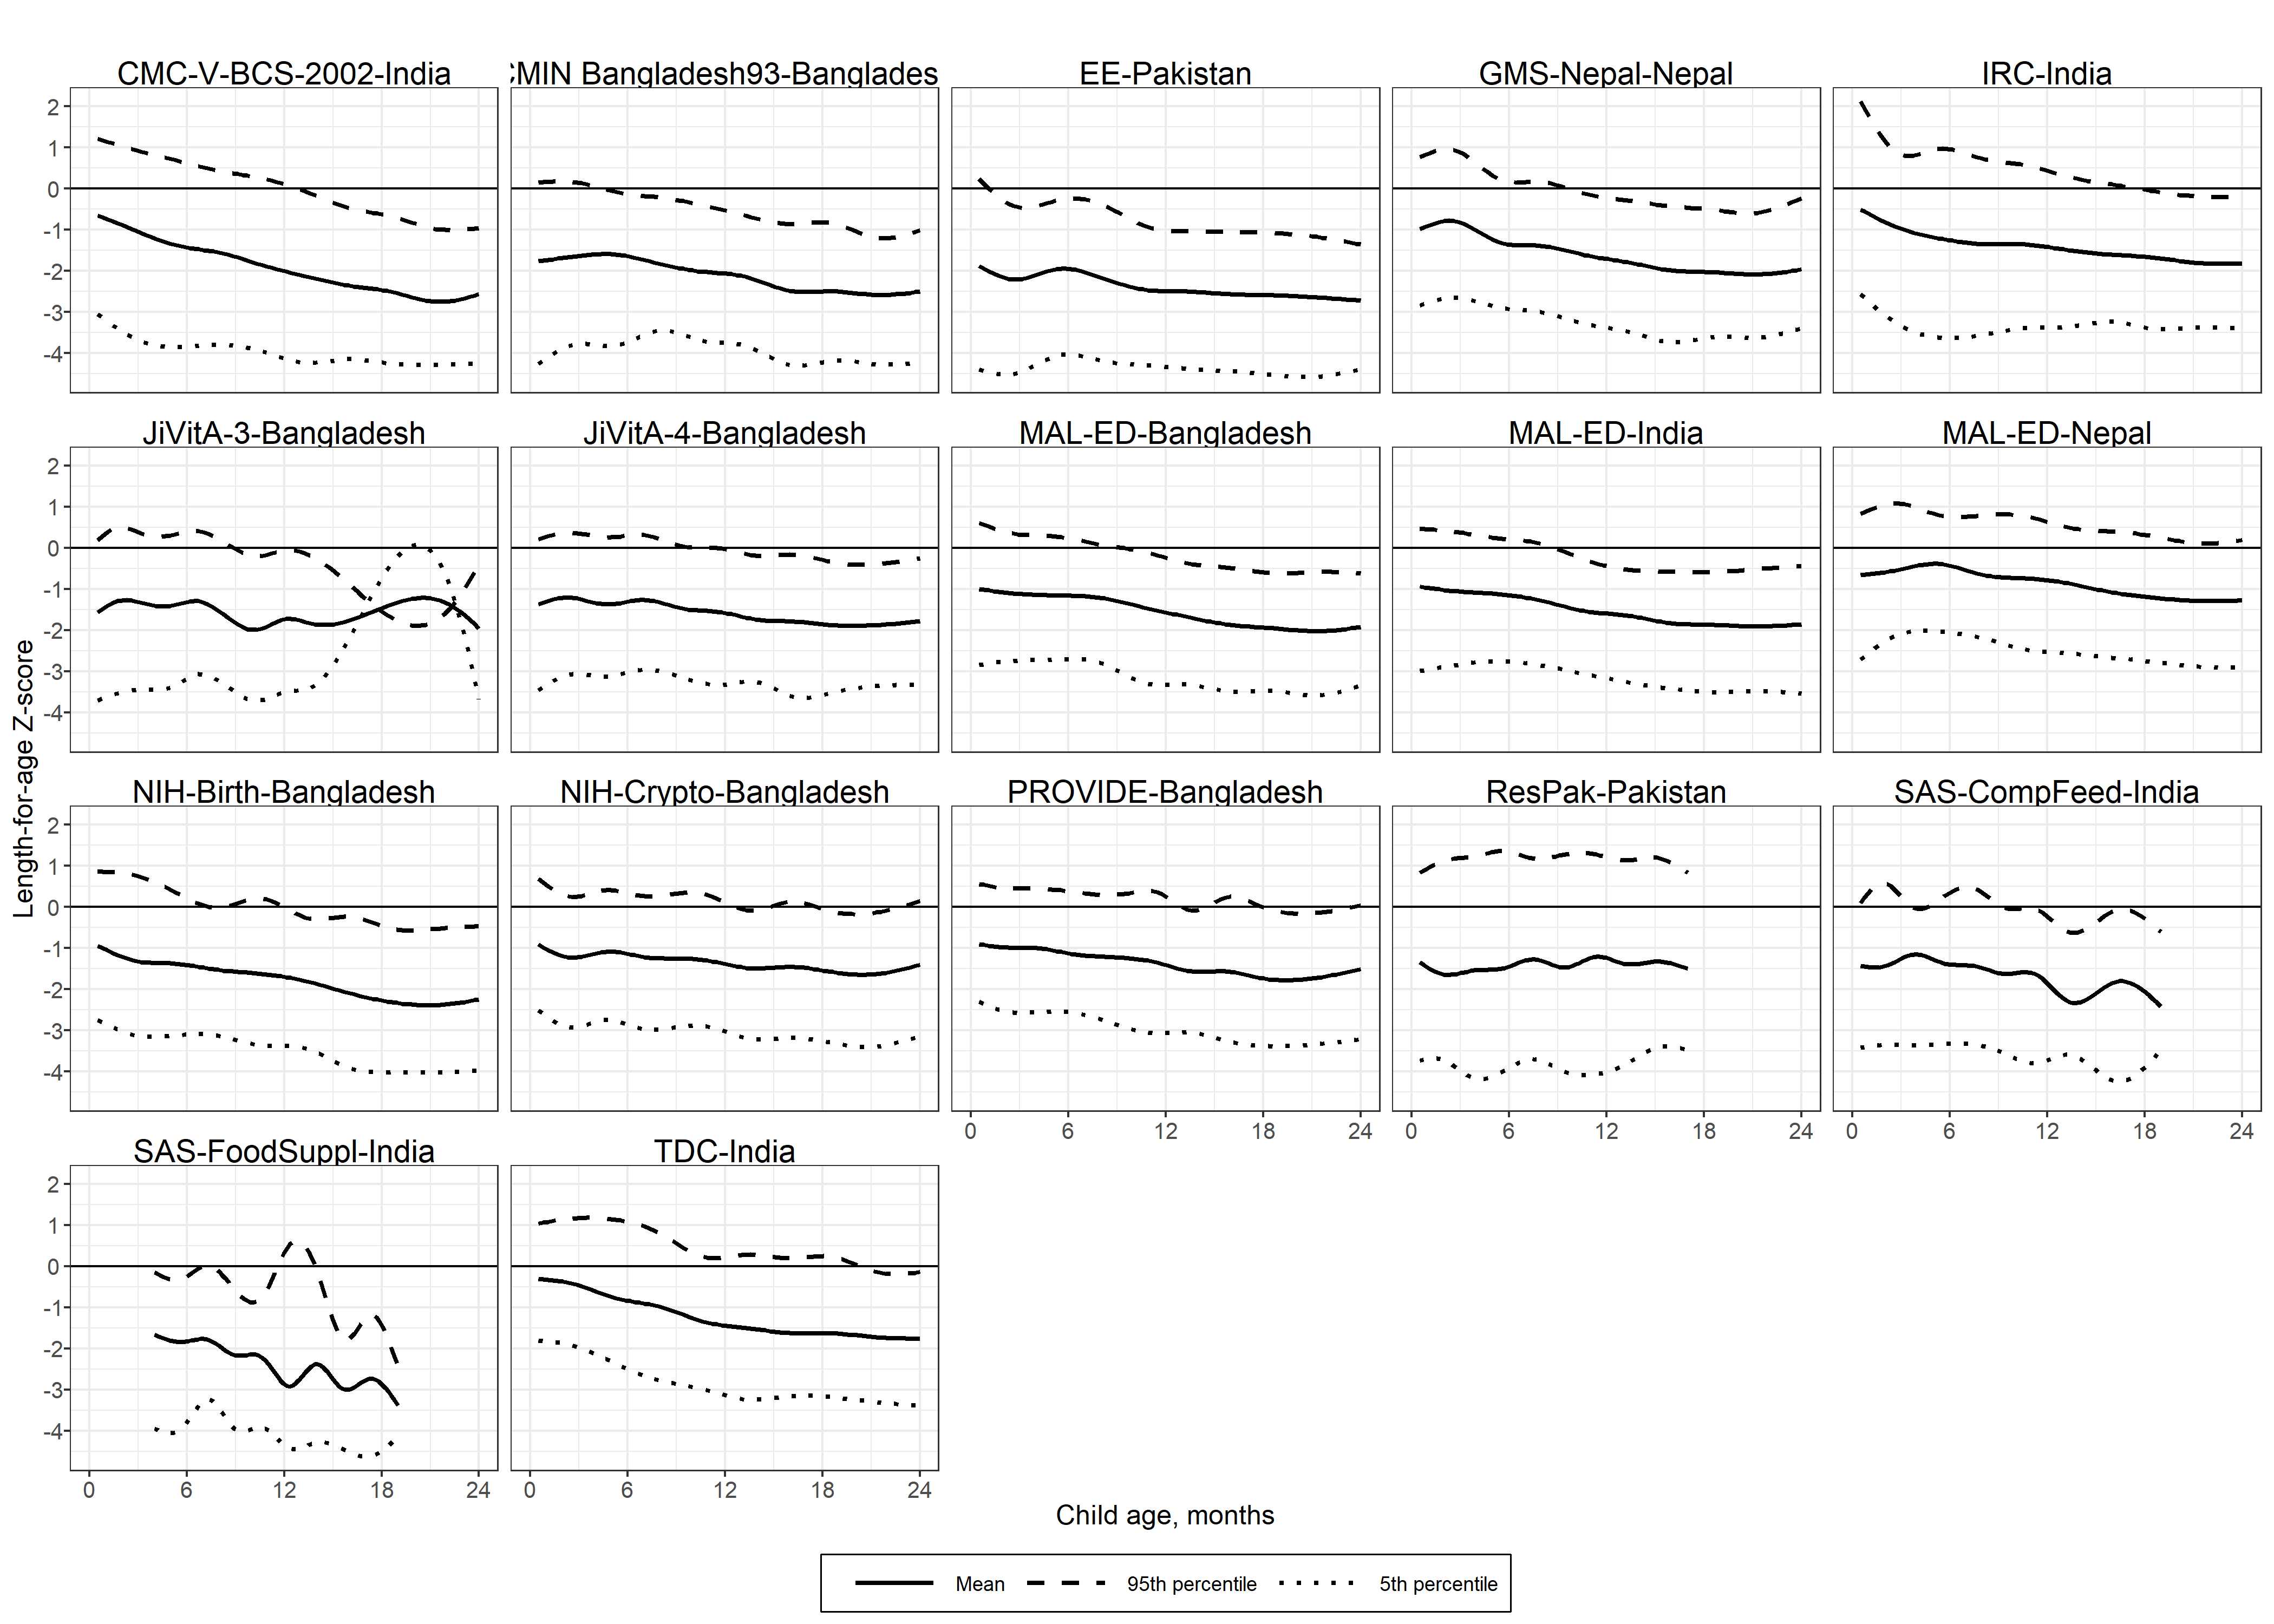
\includegraphics[width=58.33in]{C:/Users/andre/Documents/HBGDki/stunting/ki-longitudinal-manuscripts/figures/stunting/fig-laz-2-quant-cohort-asia-allage-primary}

\section{Age-specific prevalence}\label{age-specific-prevalence}

\subsection{Africa}\label{africa-1}

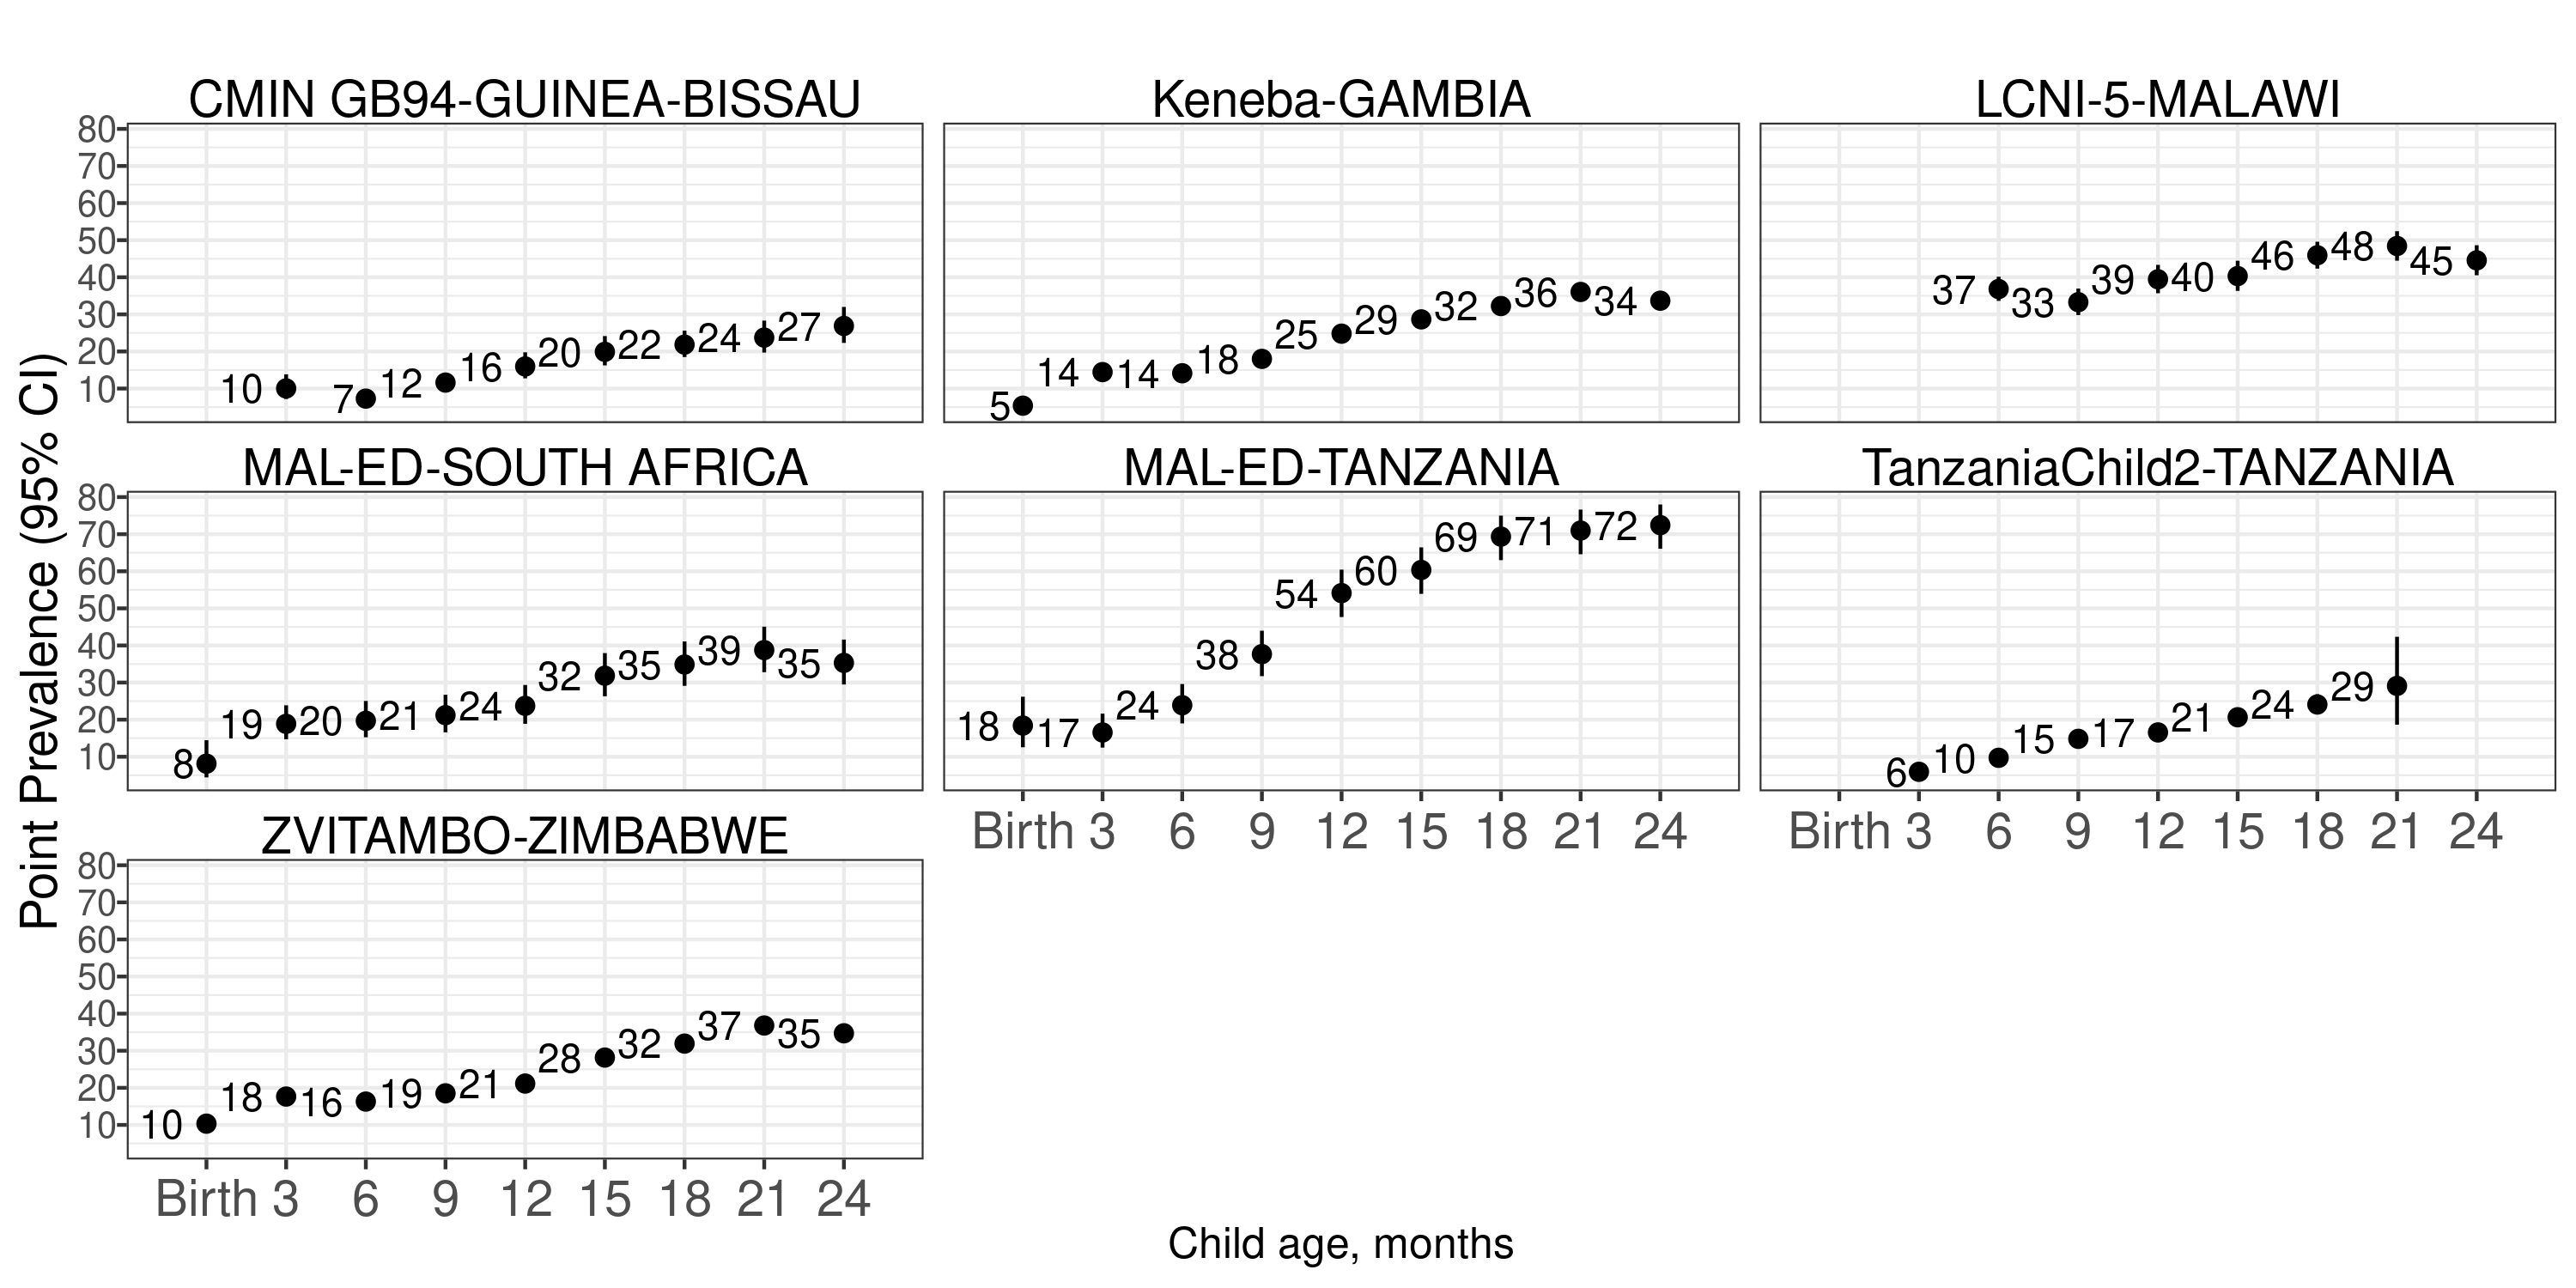
\includegraphics[width=41.67in]{C:/Users/andre/Documents/HBGDki/stunting/ki-longitudinal-manuscripts/figures/stunting/fig-stunt-2-prev-cohort-africa-allage-primary}

\subsection{Latin America}\label{latin-america-1}

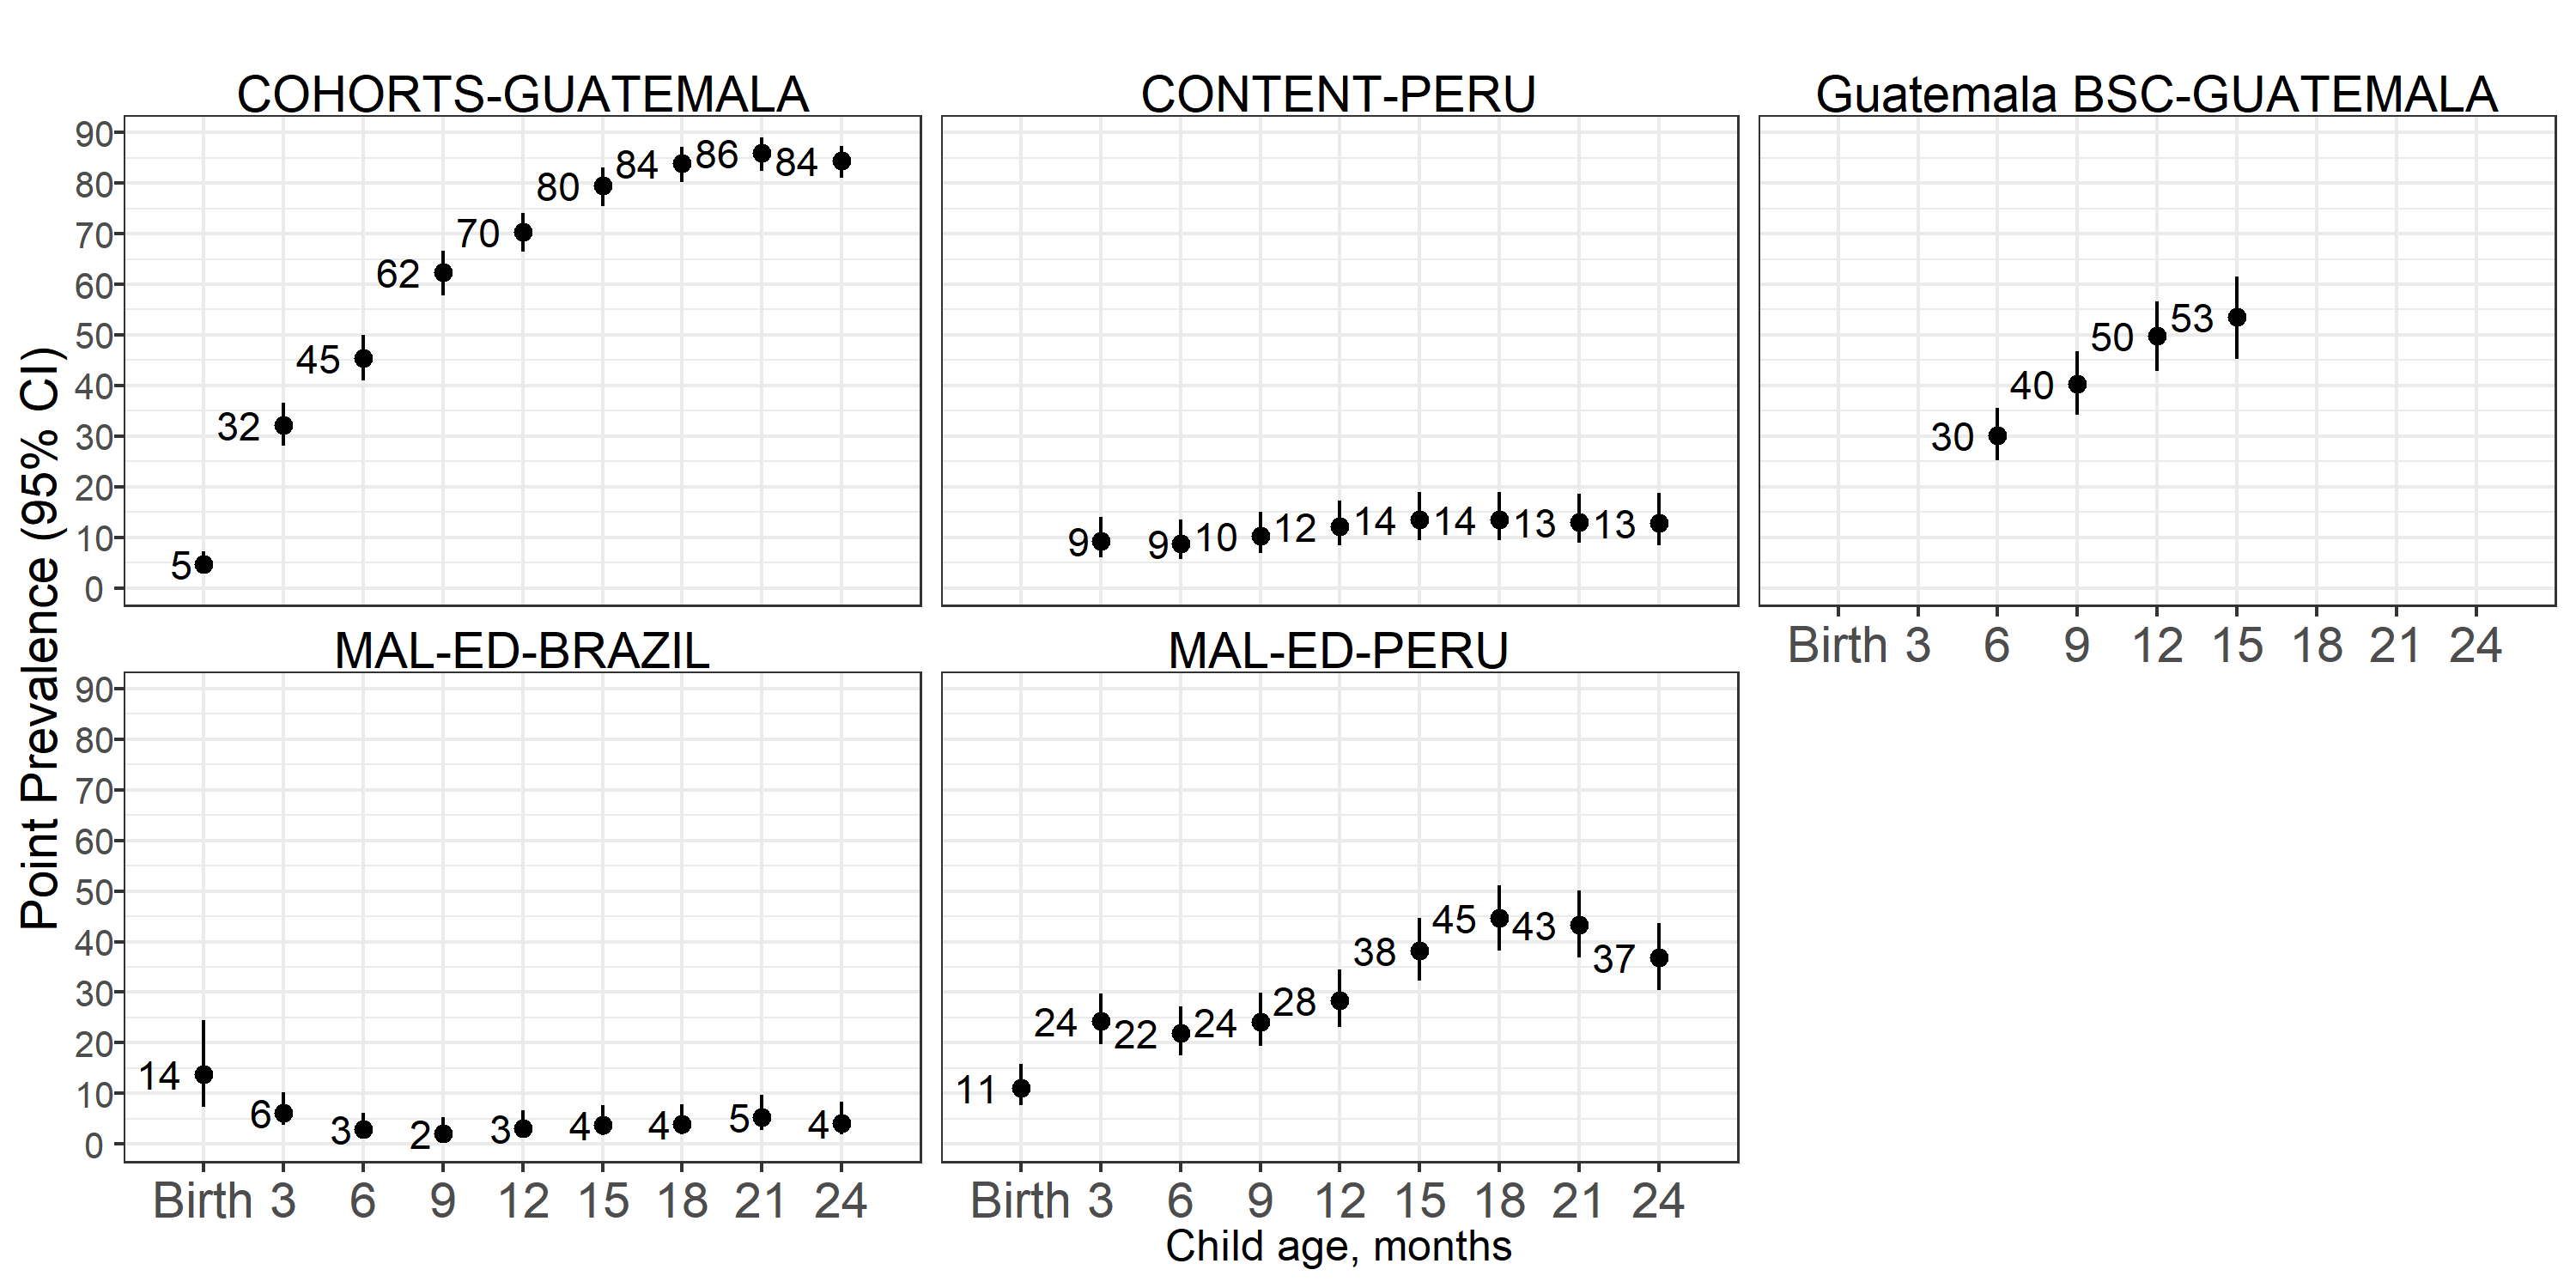
\includegraphics[width=41.67in]{C:/Users/andre/Documents/HBGDki/stunting/ki-longitudinal-manuscripts/figures/stunting/fig-stunt-2-prev-cohort-latamer-allage-primary}

\subsection{South Asia}\label{south-asia-1}

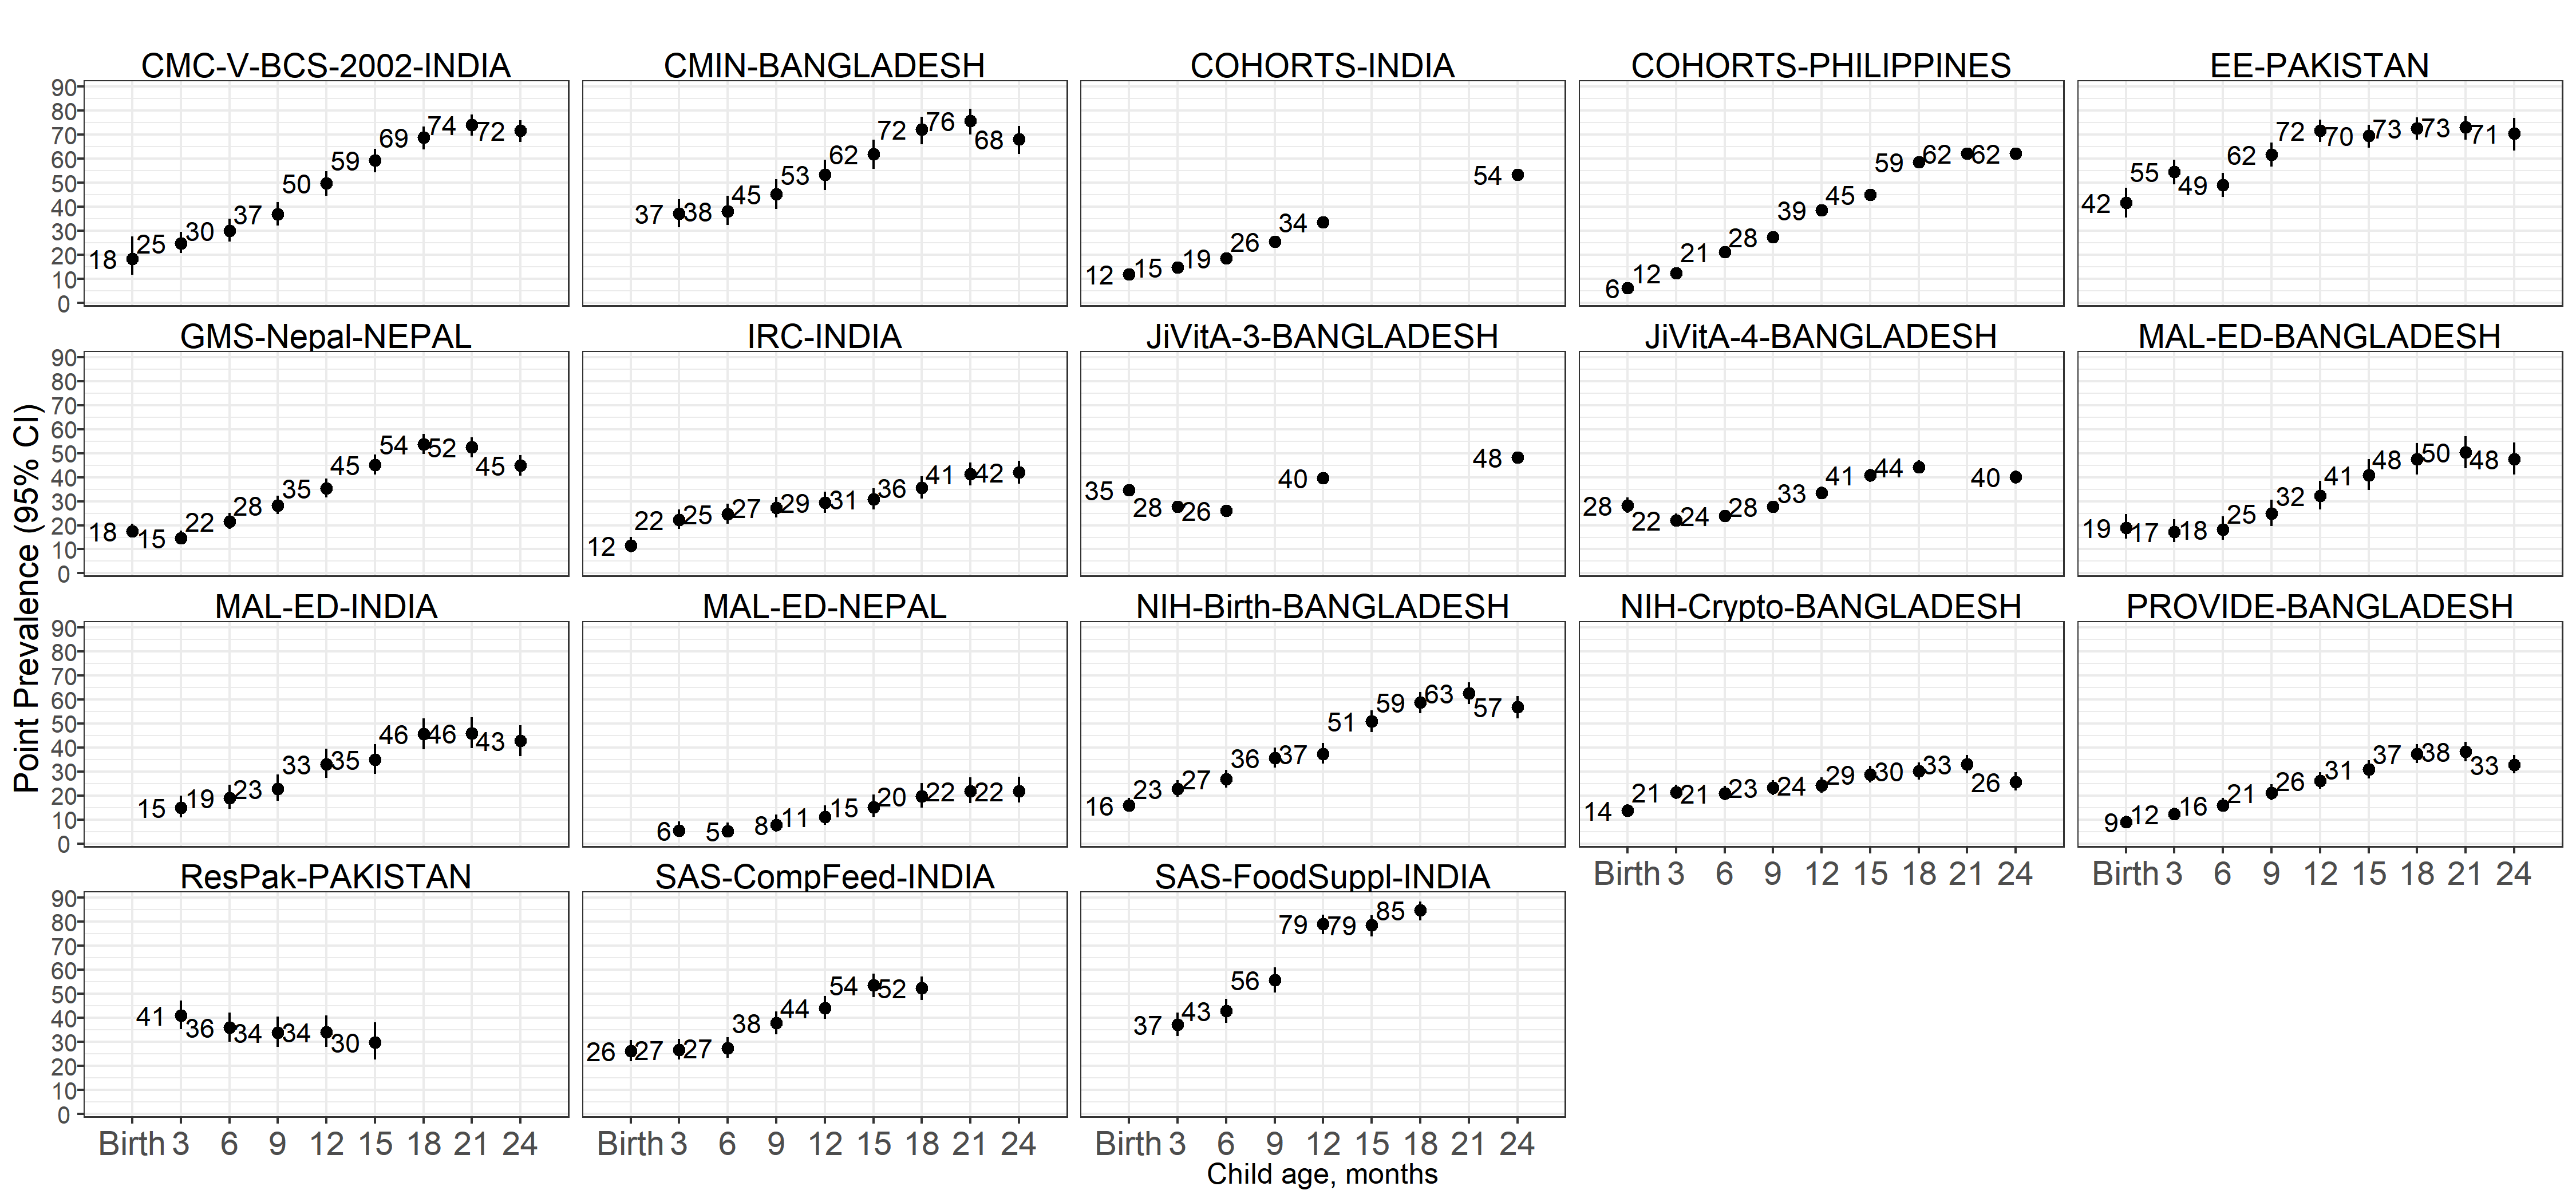
\includegraphics[width=62.5in]{C:/Users/andre/Documents/HBGDki/stunting/ki-longitudinal-manuscripts/figures/stunting/fig-stunt-2-prev-cohort-asia-allage-primary}

\section{Age-specific incidence}\label{age-specific-incidence}

\subsection{Africa}\label{africa-2}


\includegraphics[width=41.67in]{C:/Users/andre/Documents/HBGDki/stunting/ki-longitudinal-manuscripts/figures/stunting/fig-stunt-2-inc-cohort-africa-allage-primary}

\subsection{Latin America}\label{latin-america-2}

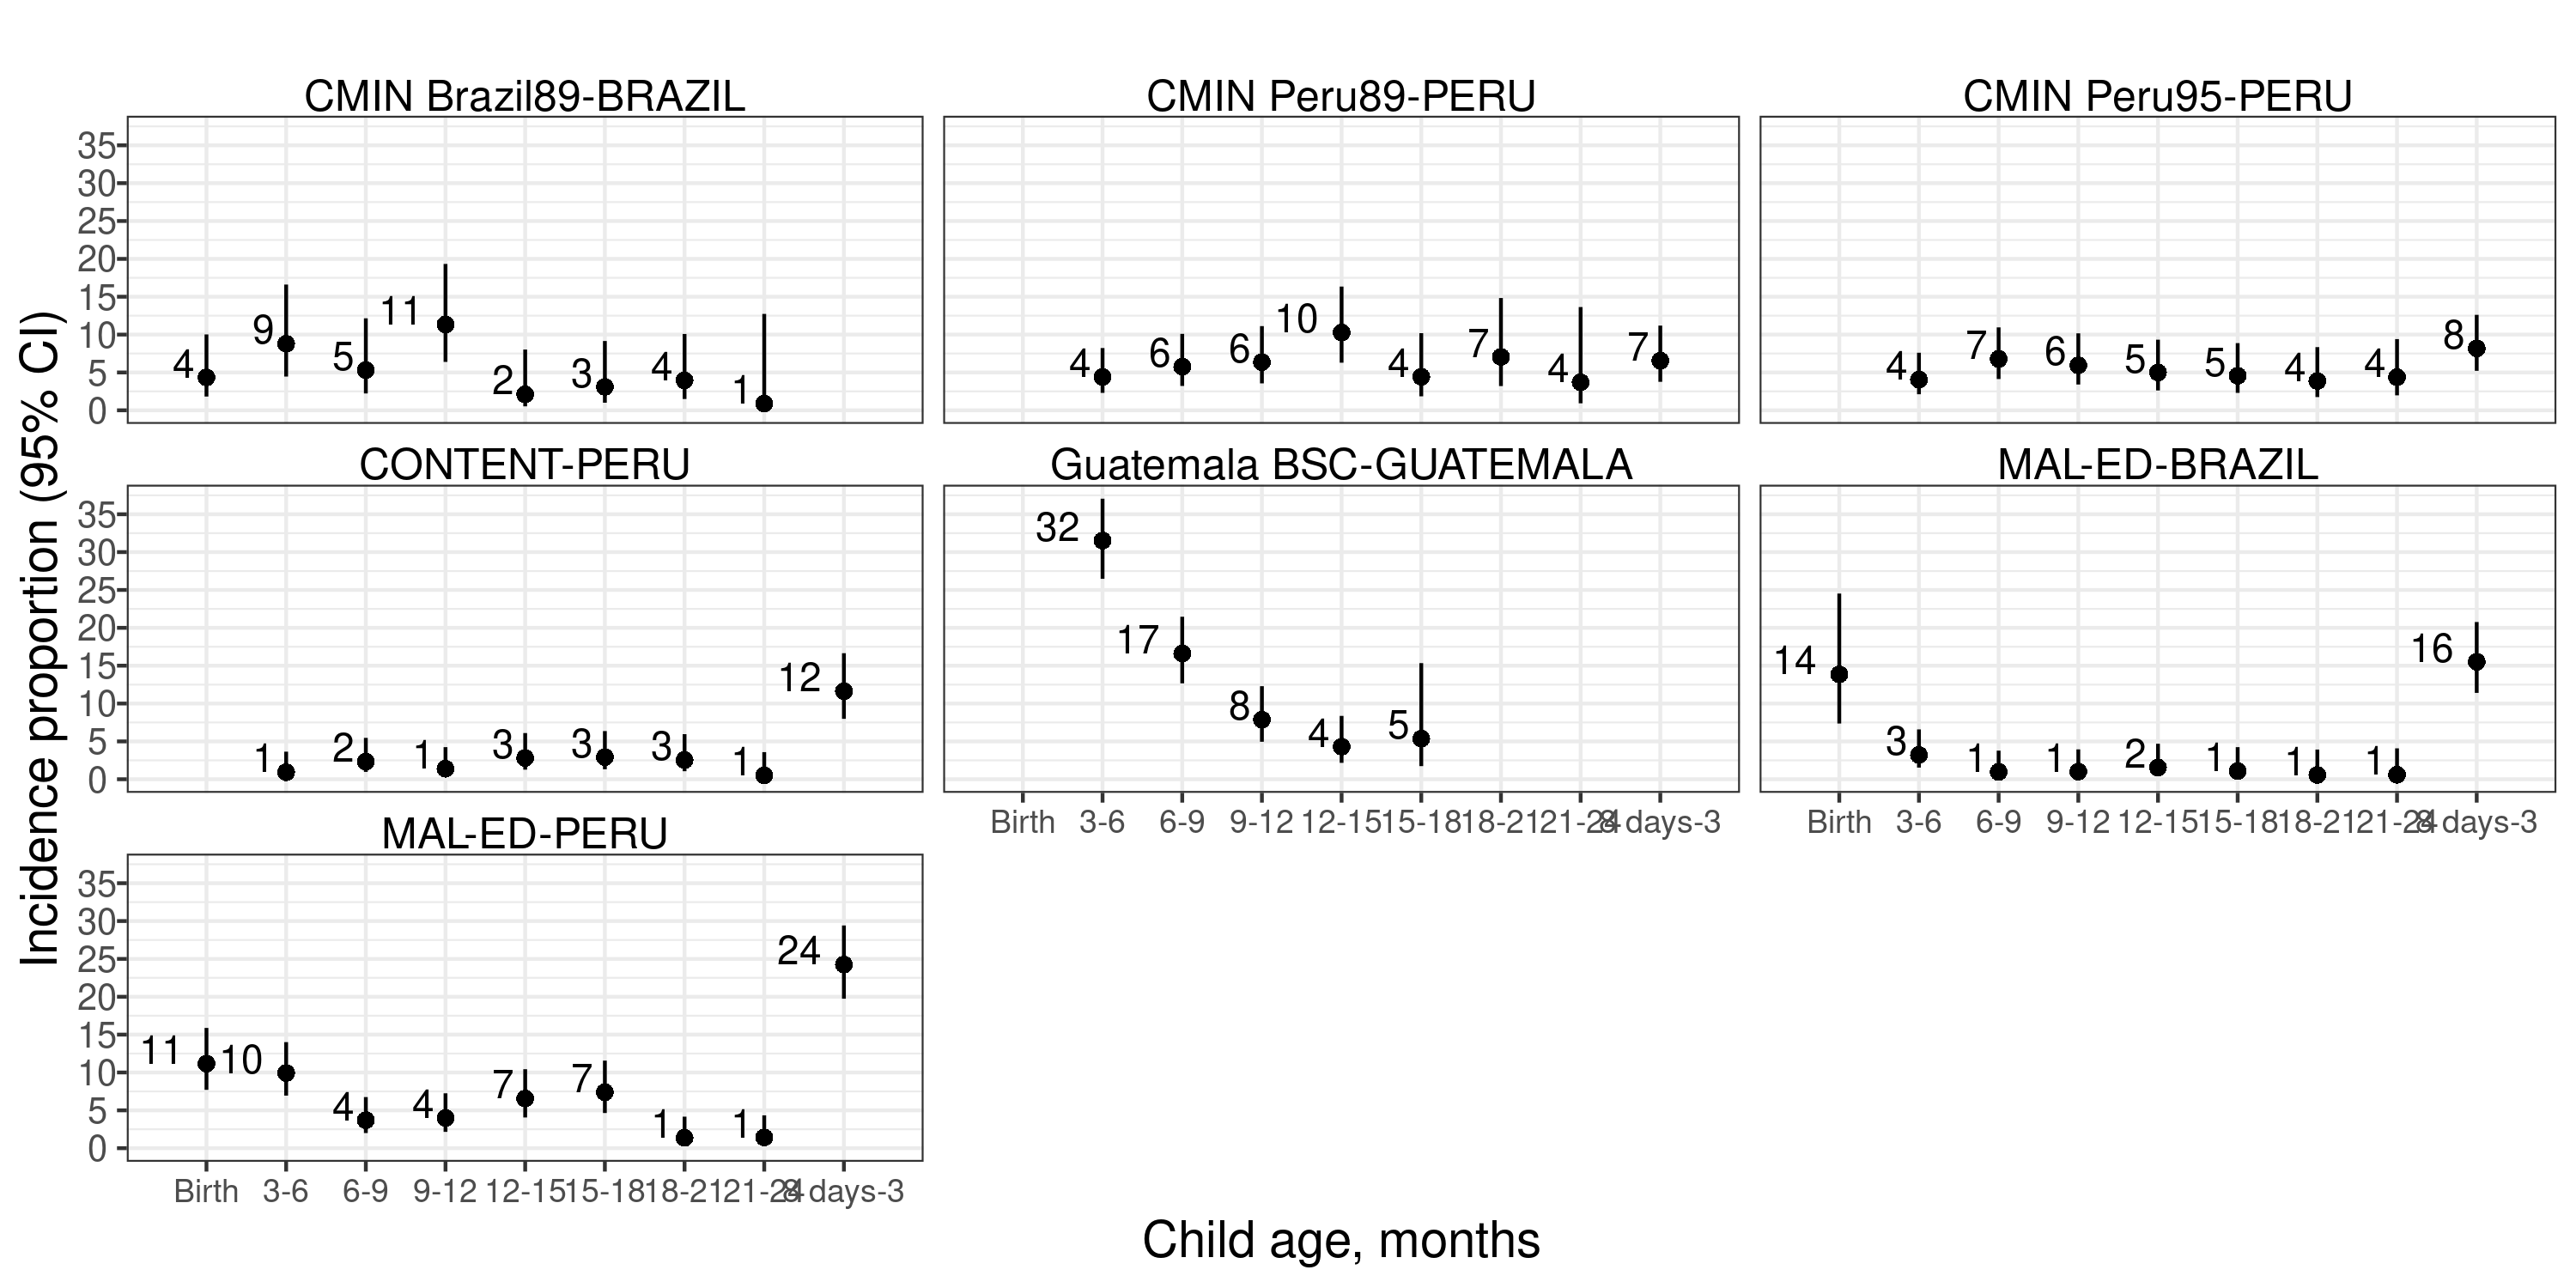
\includegraphics[width=41.67in]{C:/Users/andre/Documents/HBGDki/stunting/ki-longitudinal-manuscripts/figures/stunting/fig-stunt-2-inc-cohort-latamer-allage-primary}

\subsection{South Asia}\label{south-asia-2}

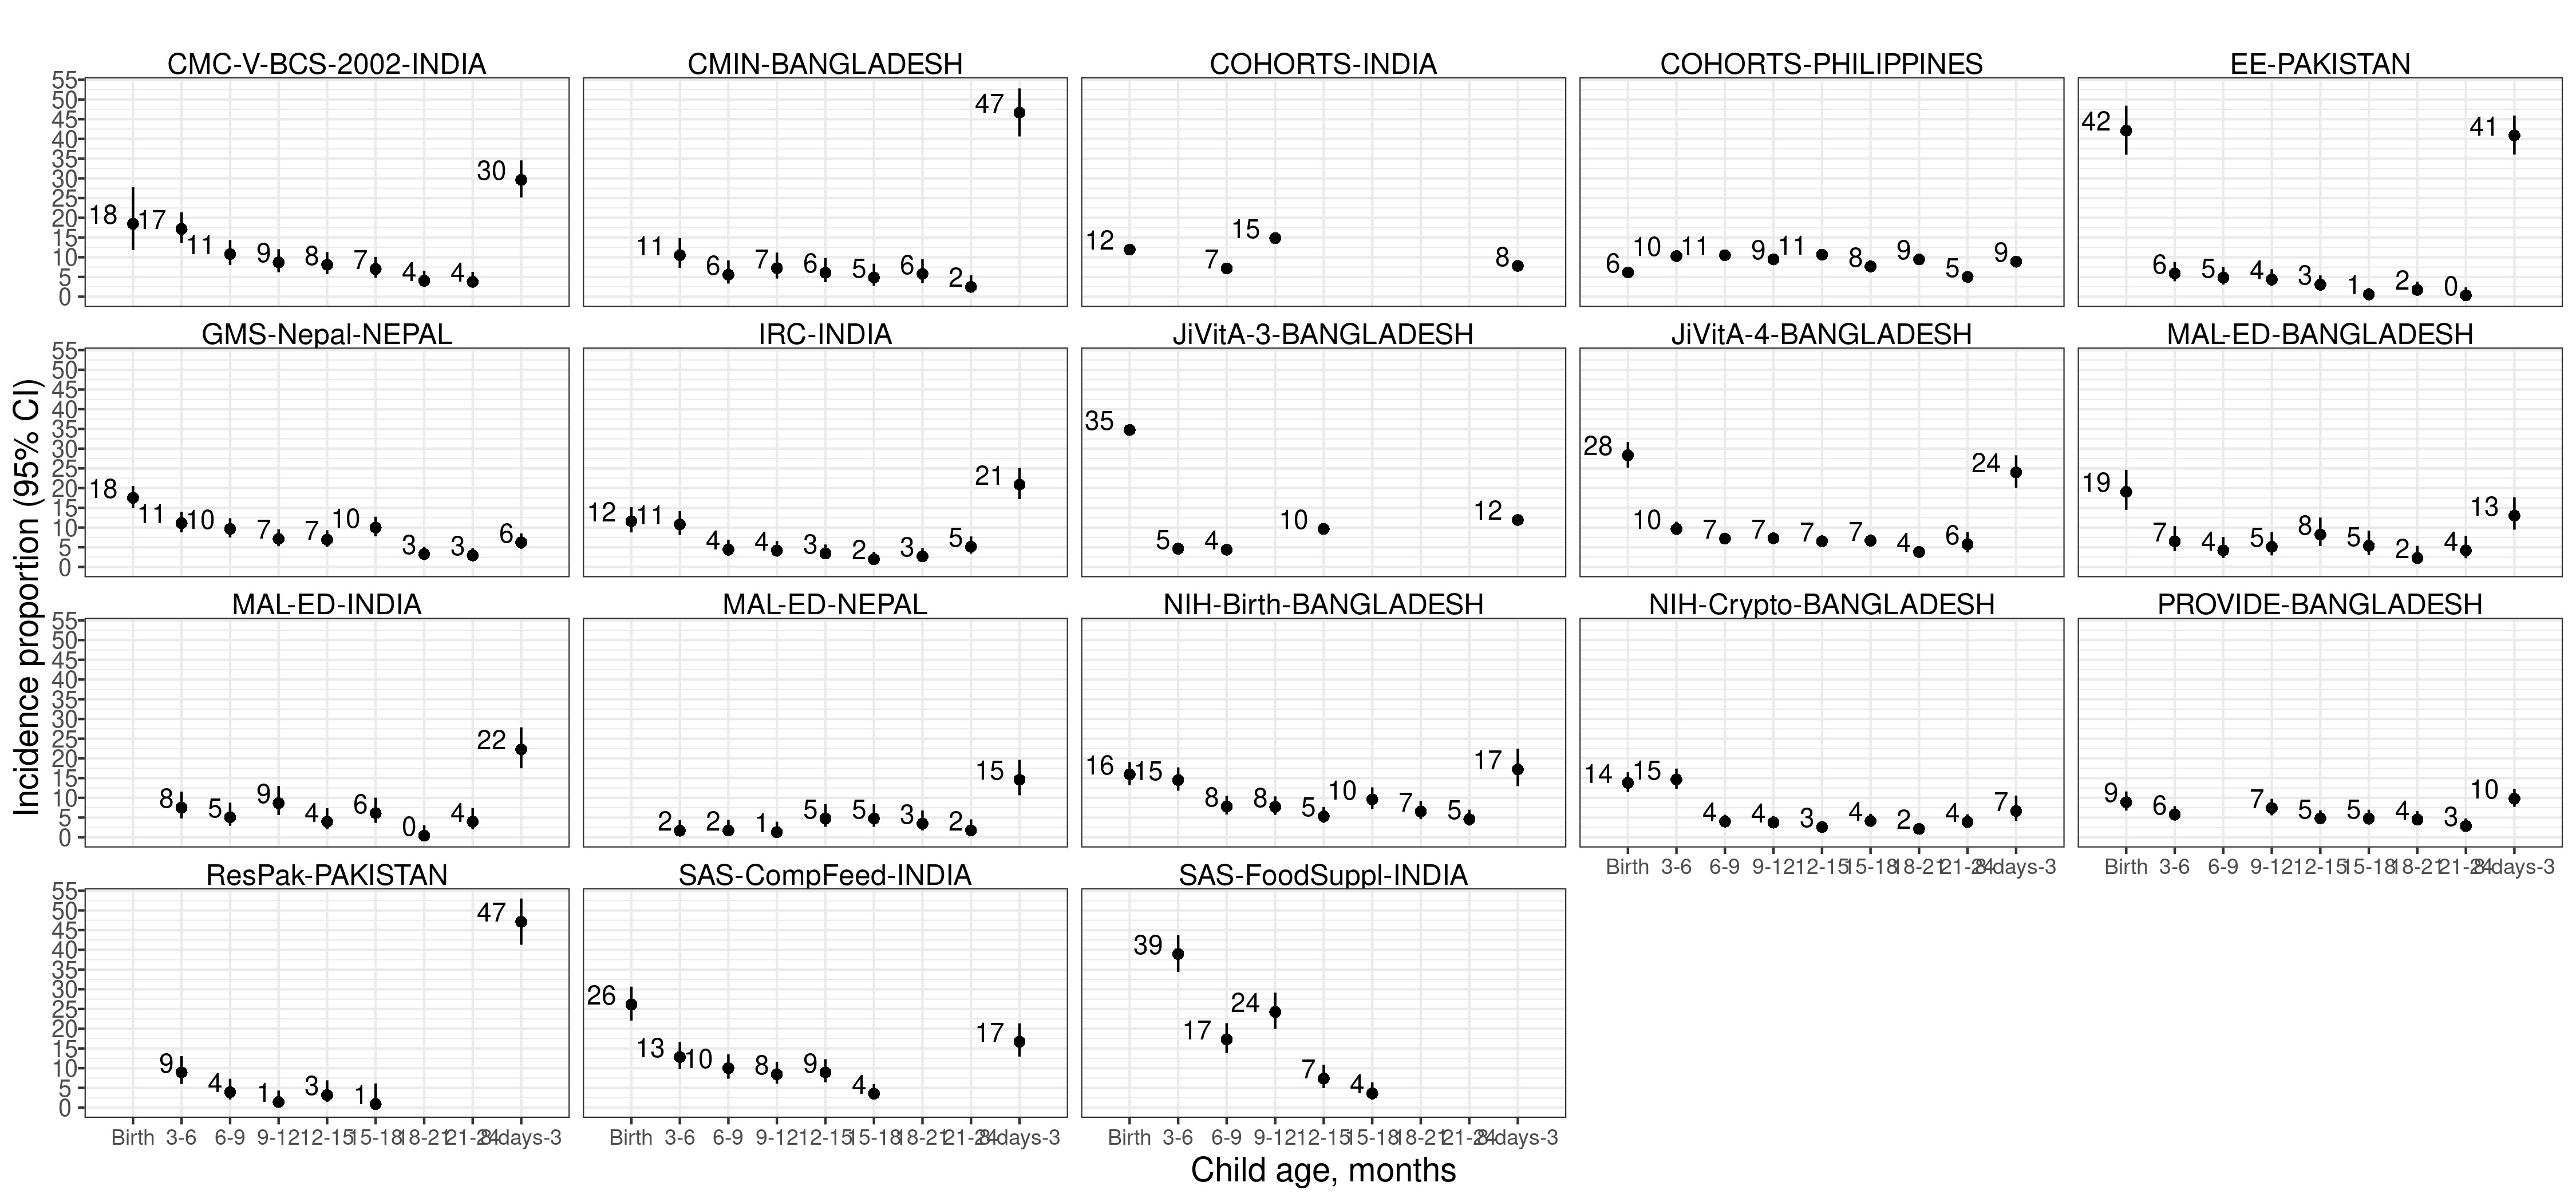
\includegraphics[width=62.5in]{C:/Users/andre/Documents/HBGDki/stunting/ki-longitudinal-manuscripts/figures/stunting/fig-stunt-2-inc-cohort-asia-allage-primary}

\section{Length velocity by age and
sex}\label{length-velocity-by-age-and-sex}

\subsection{Africa}\label{africa-3}

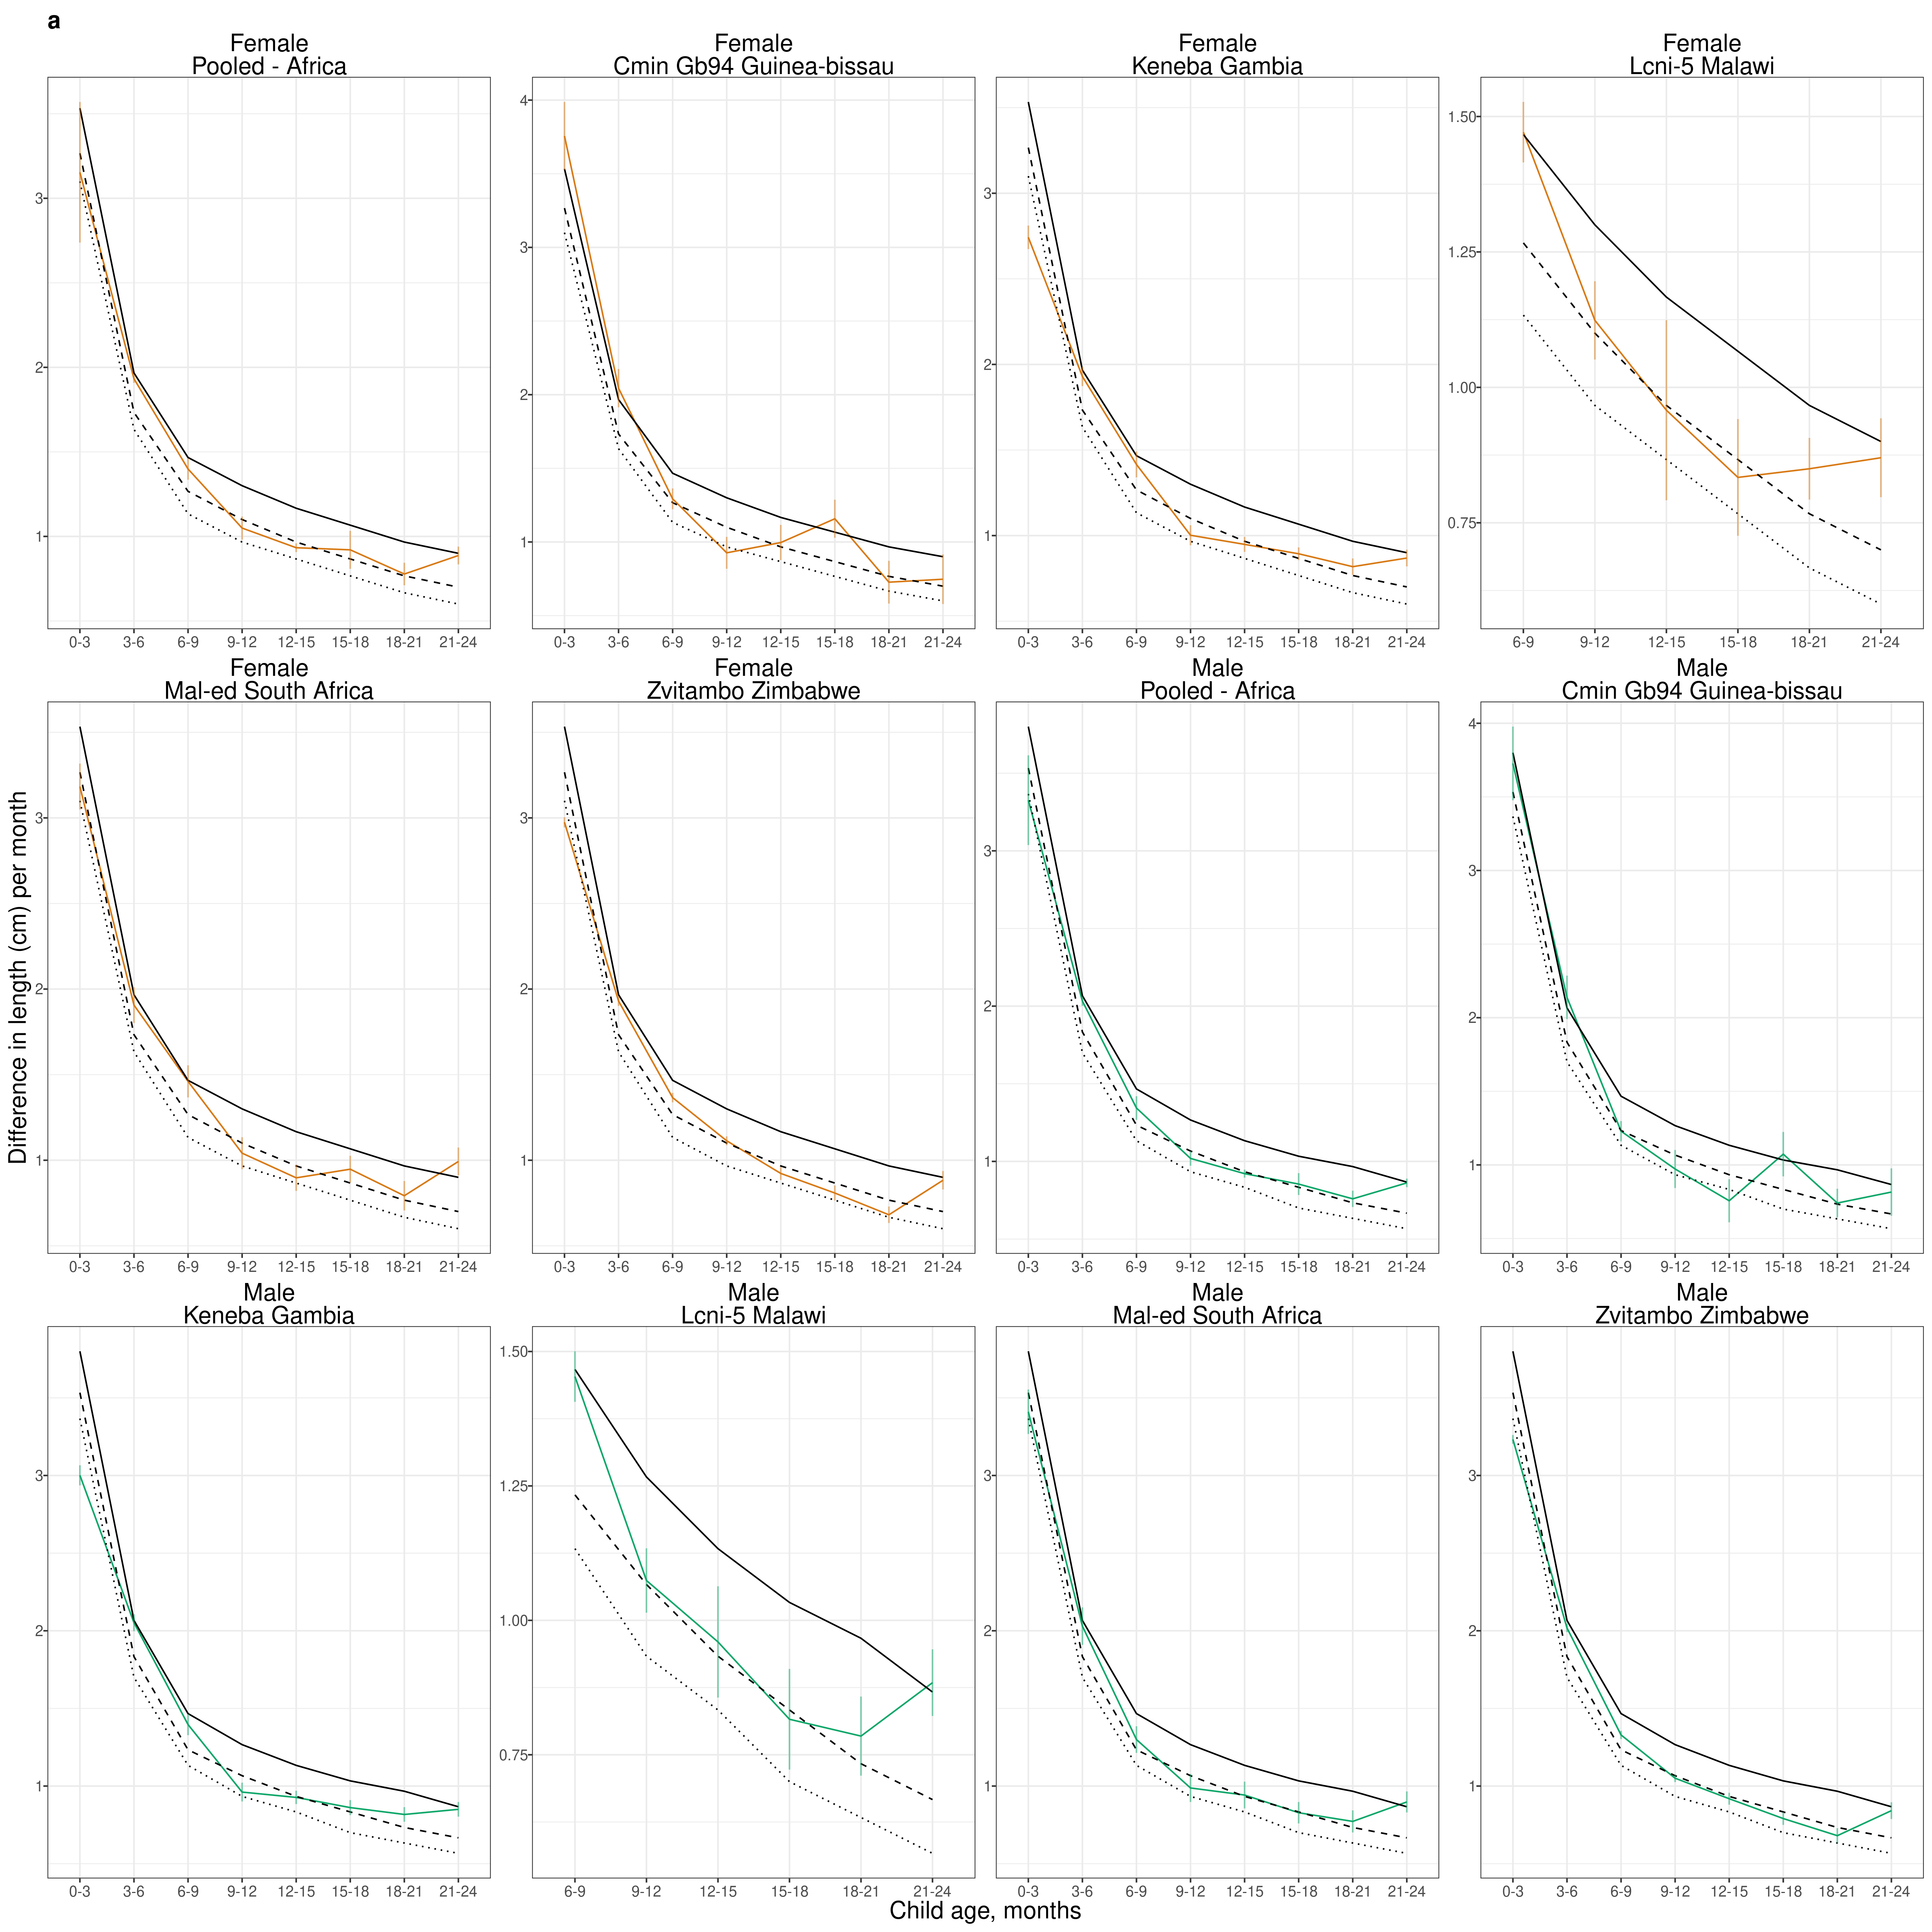
\includegraphics[width=75in]{C:/Users/andre/Documents/HBGDki/stunting/ki-longitudinal-manuscripts/figures/stunting/fig-length-2-length_vel-cohort-africa-allage-primary}
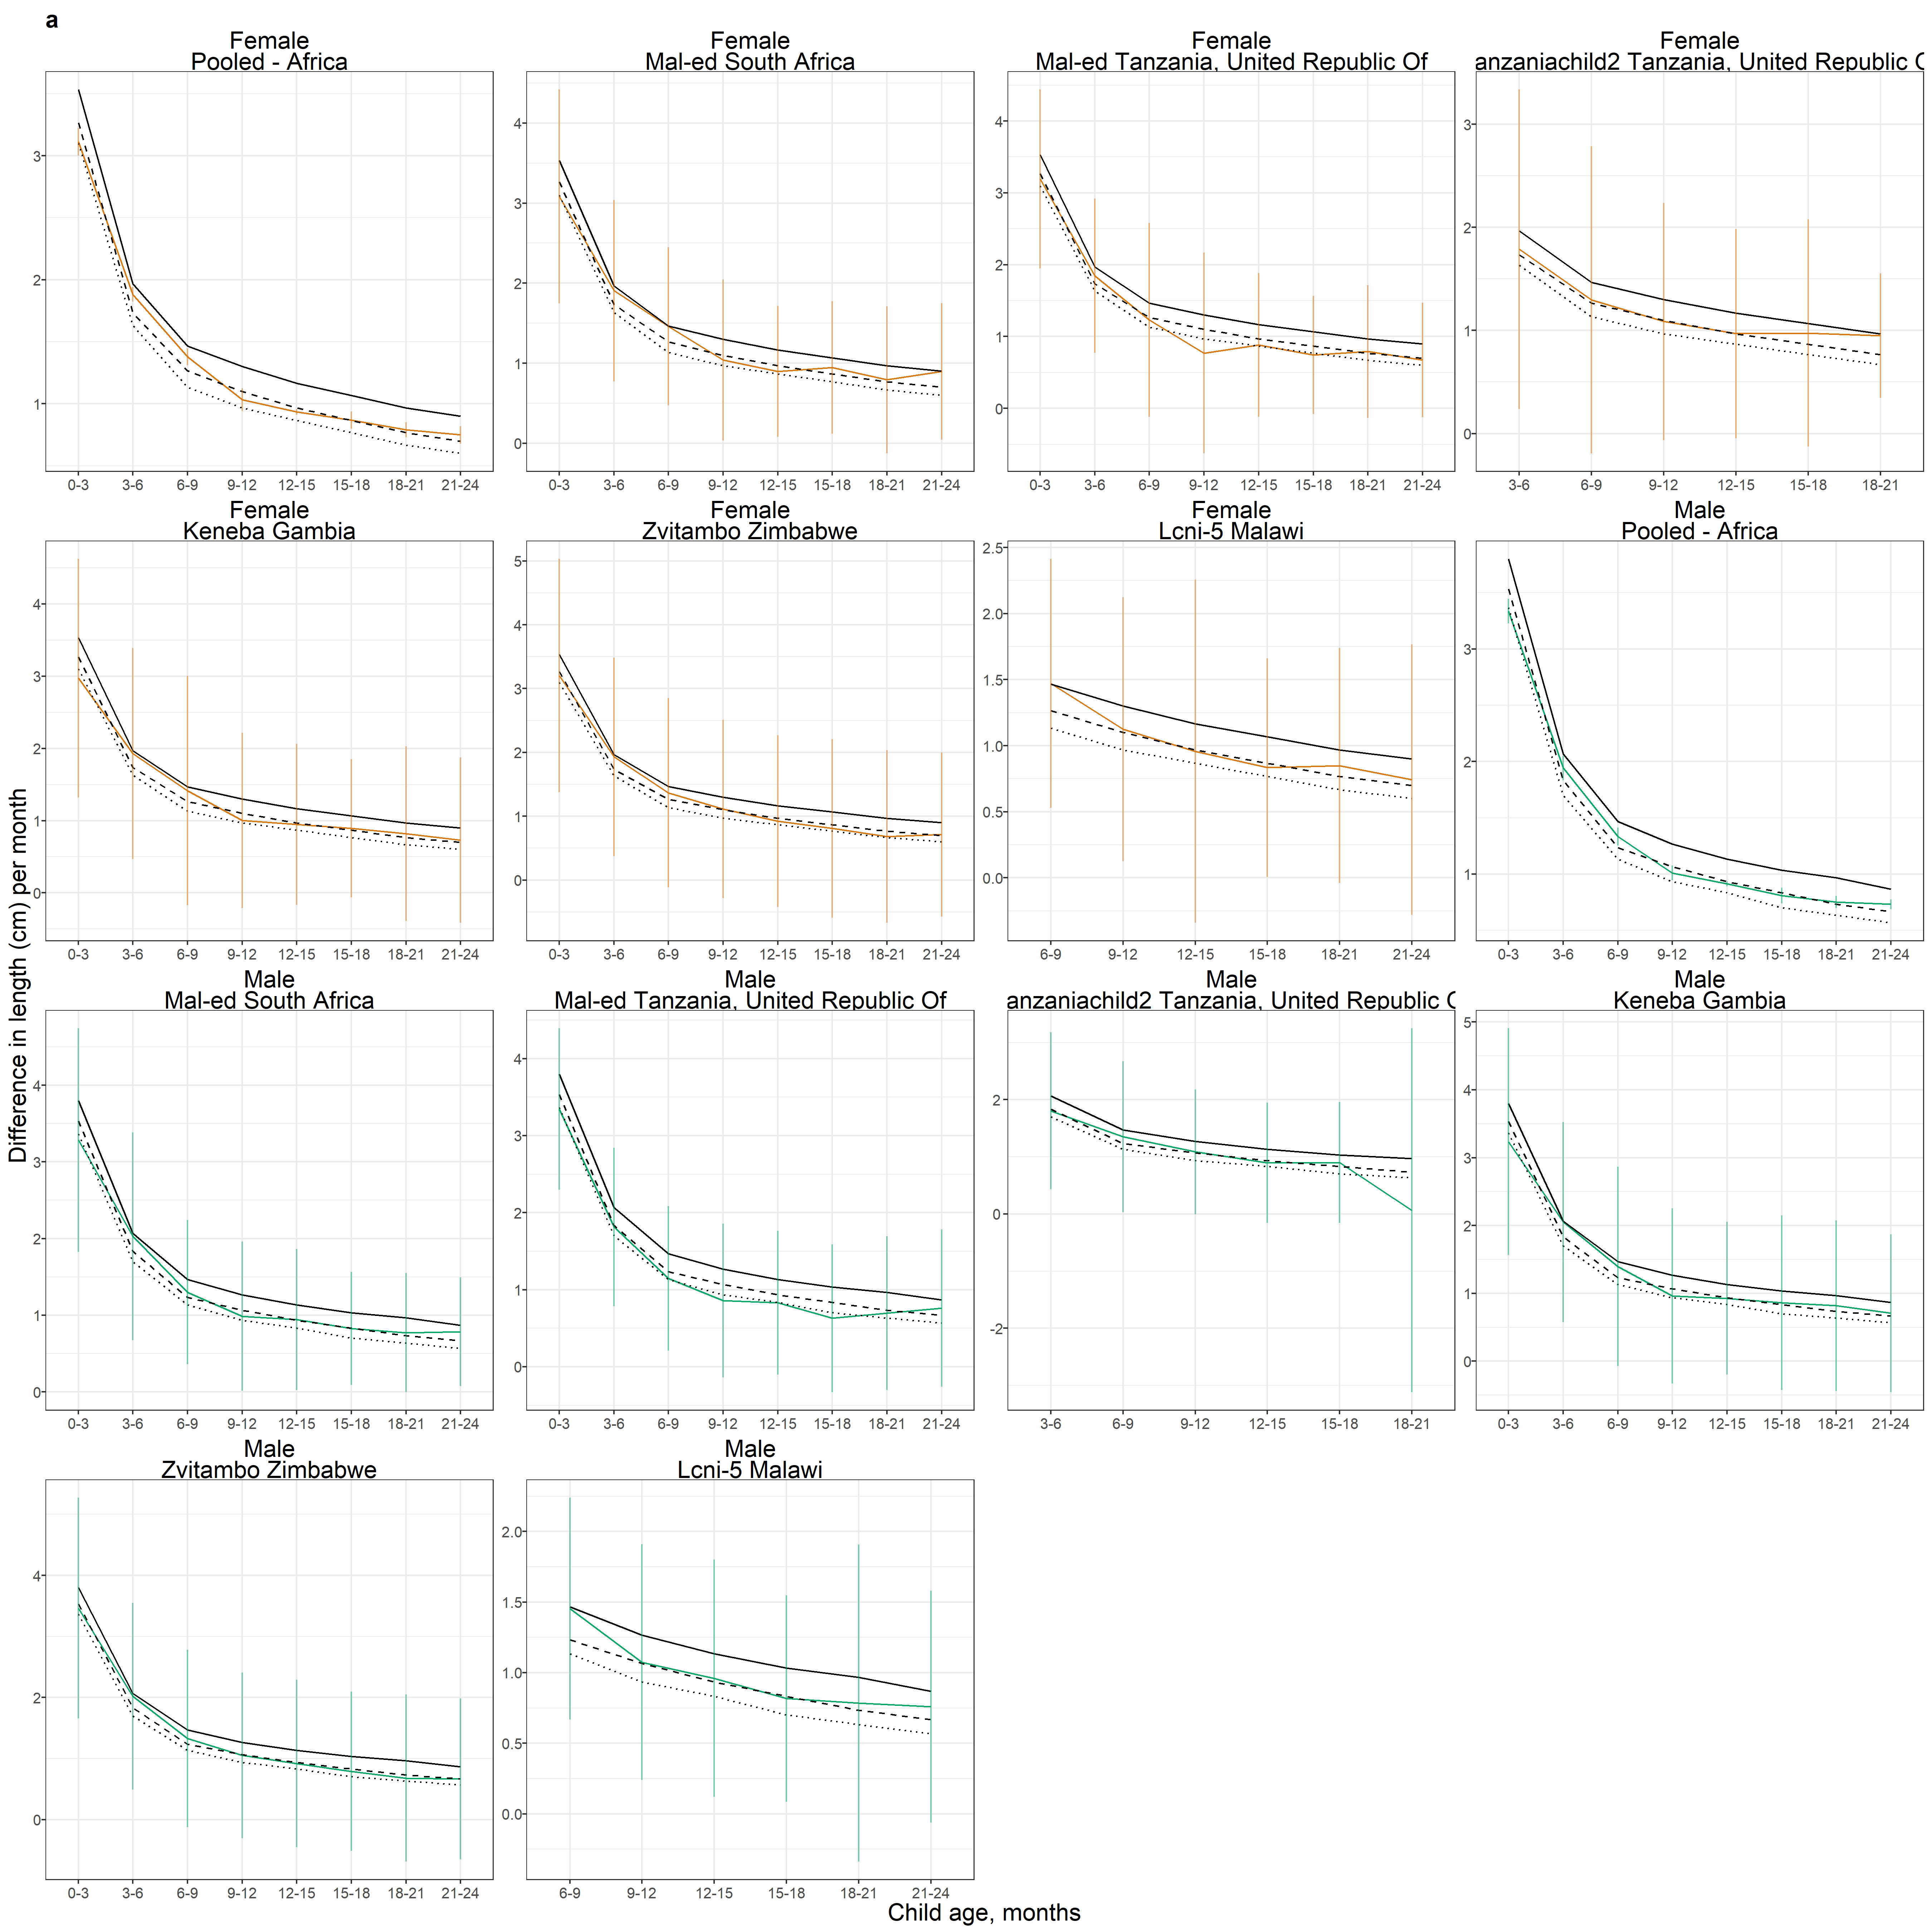
\includegraphics[width=75in]{figure-copies/fig-length-2-length_vel-cohort-africa-allage-primary}

\subsection{Latin America}\label{latin-america-3}

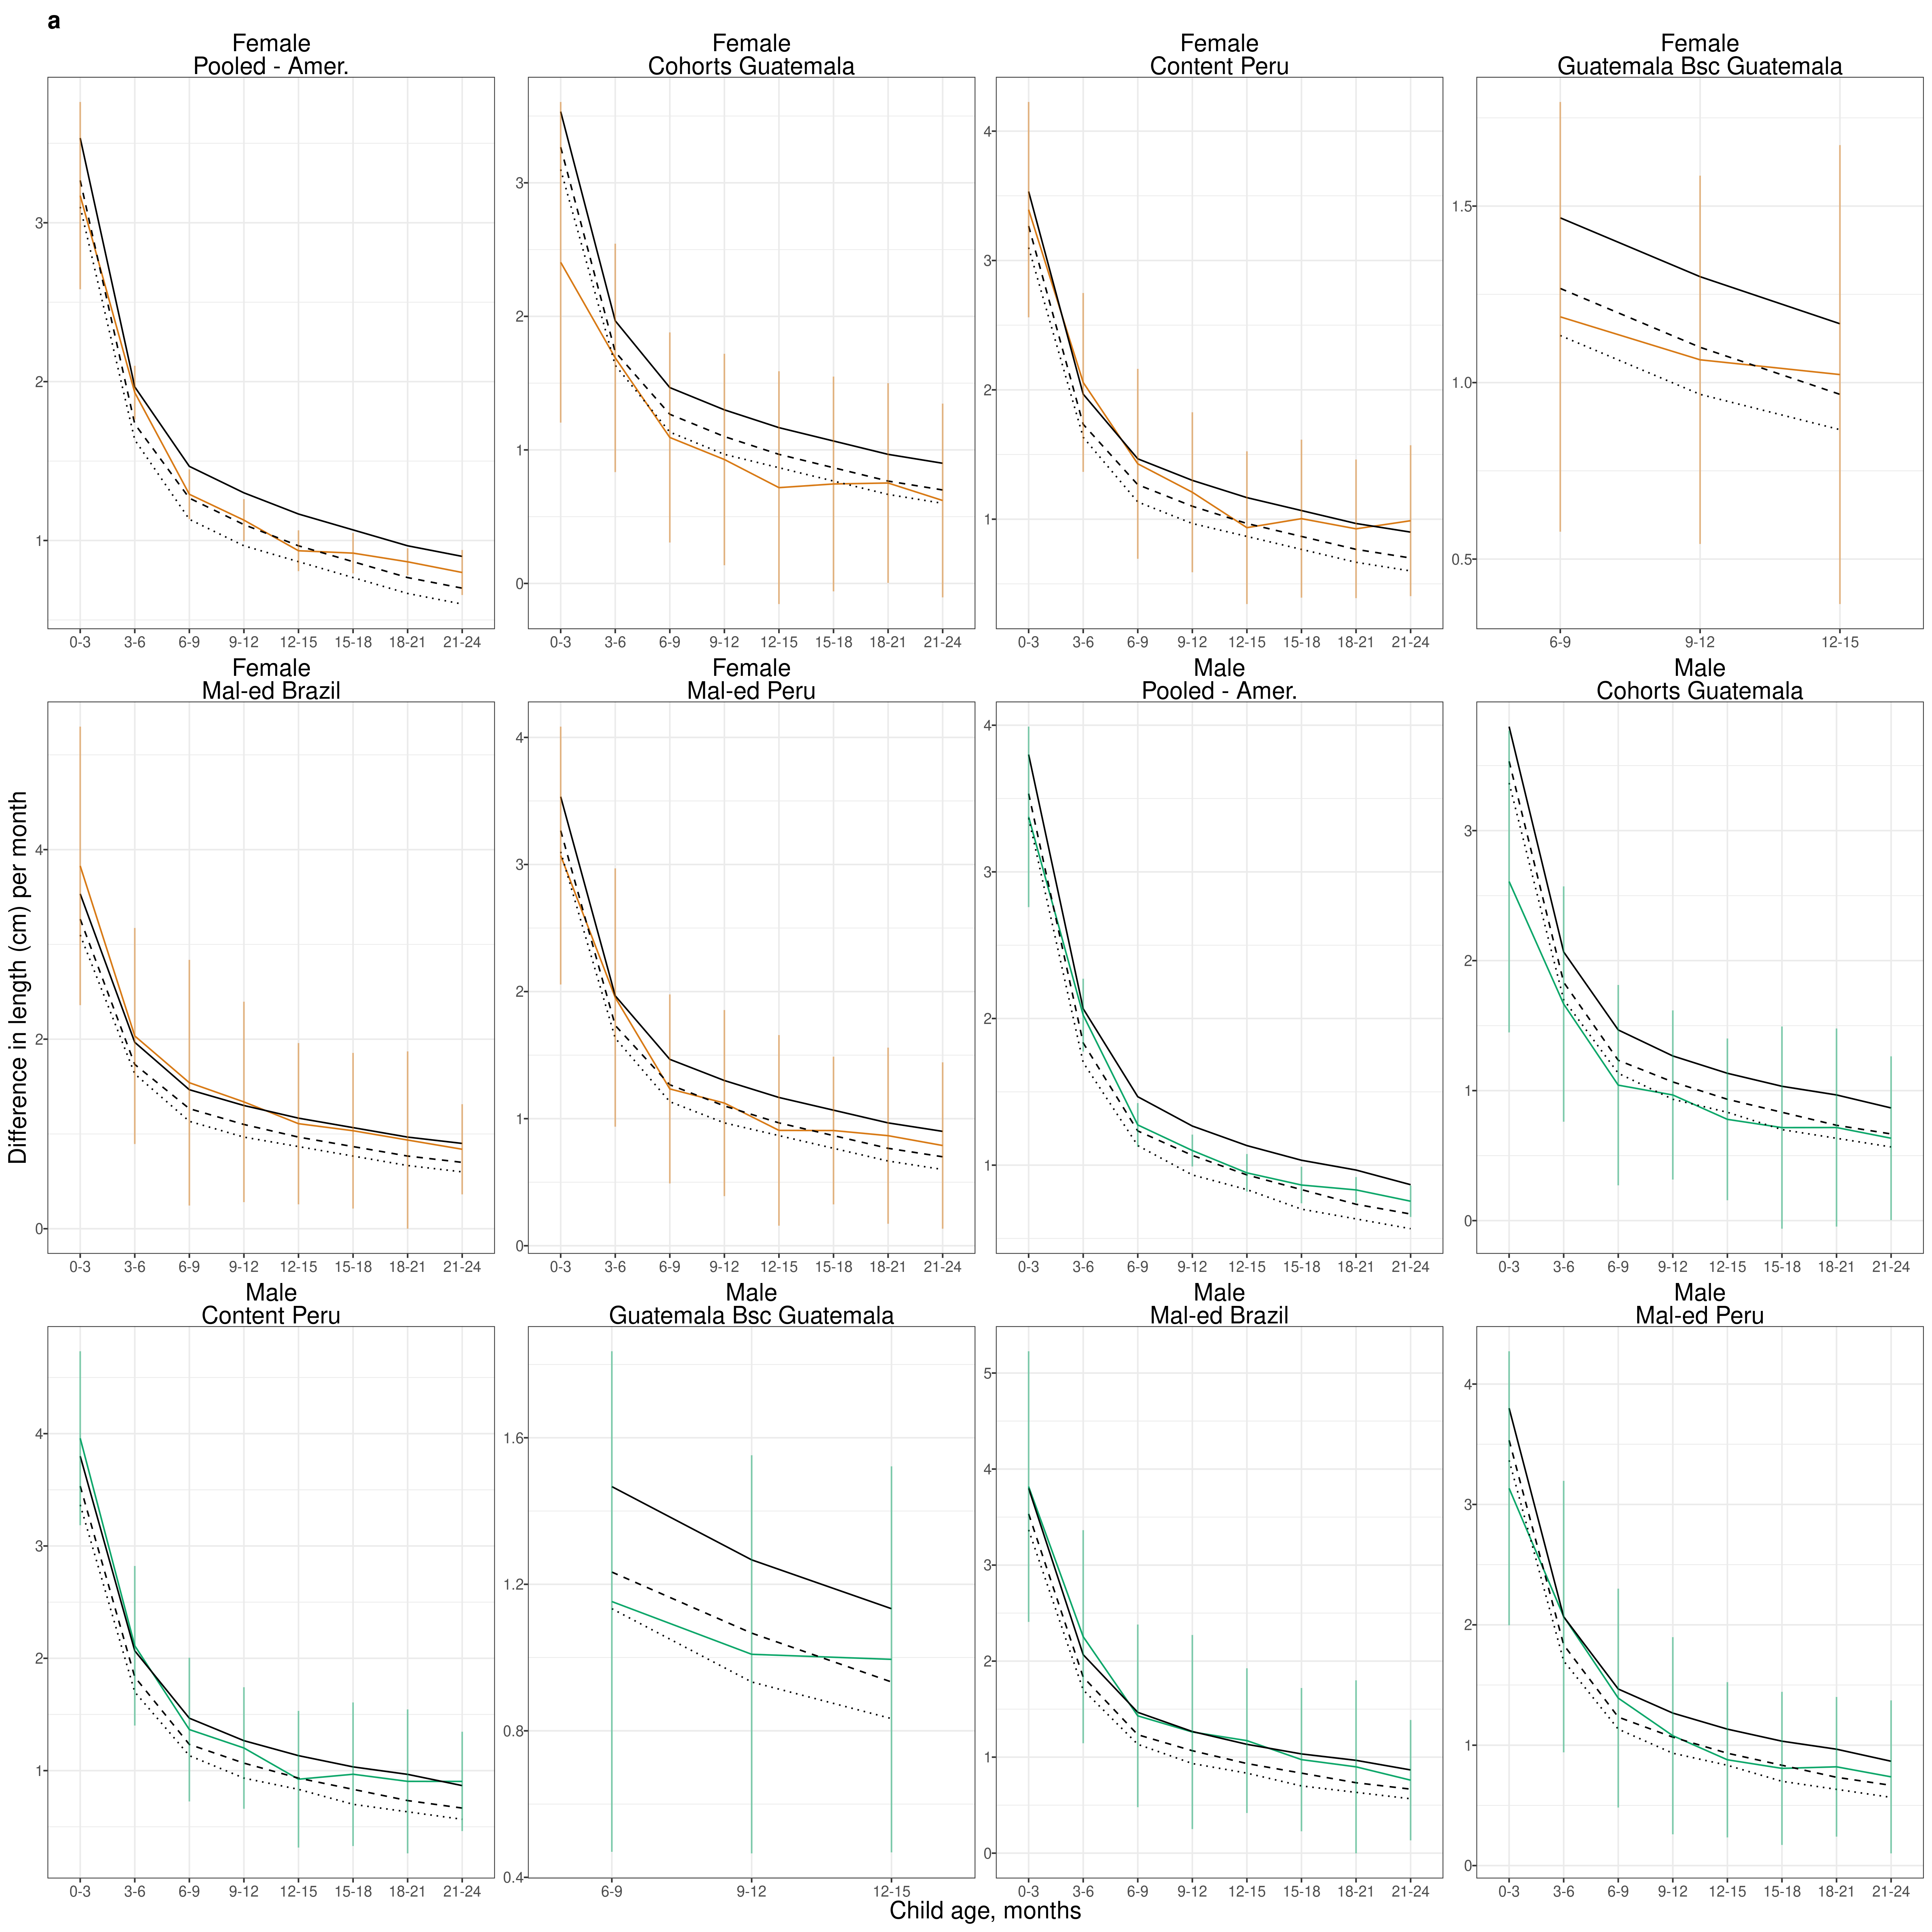
\includegraphics[width=75in]{C:/Users/andre/Documents/HBGDki/stunting/ki-longitudinal-manuscripts/figures/stunting/fig-length-2-length_vel-cohort-latamer-allage-primary}

\subsection{South Asia}\label{south-asia-3}

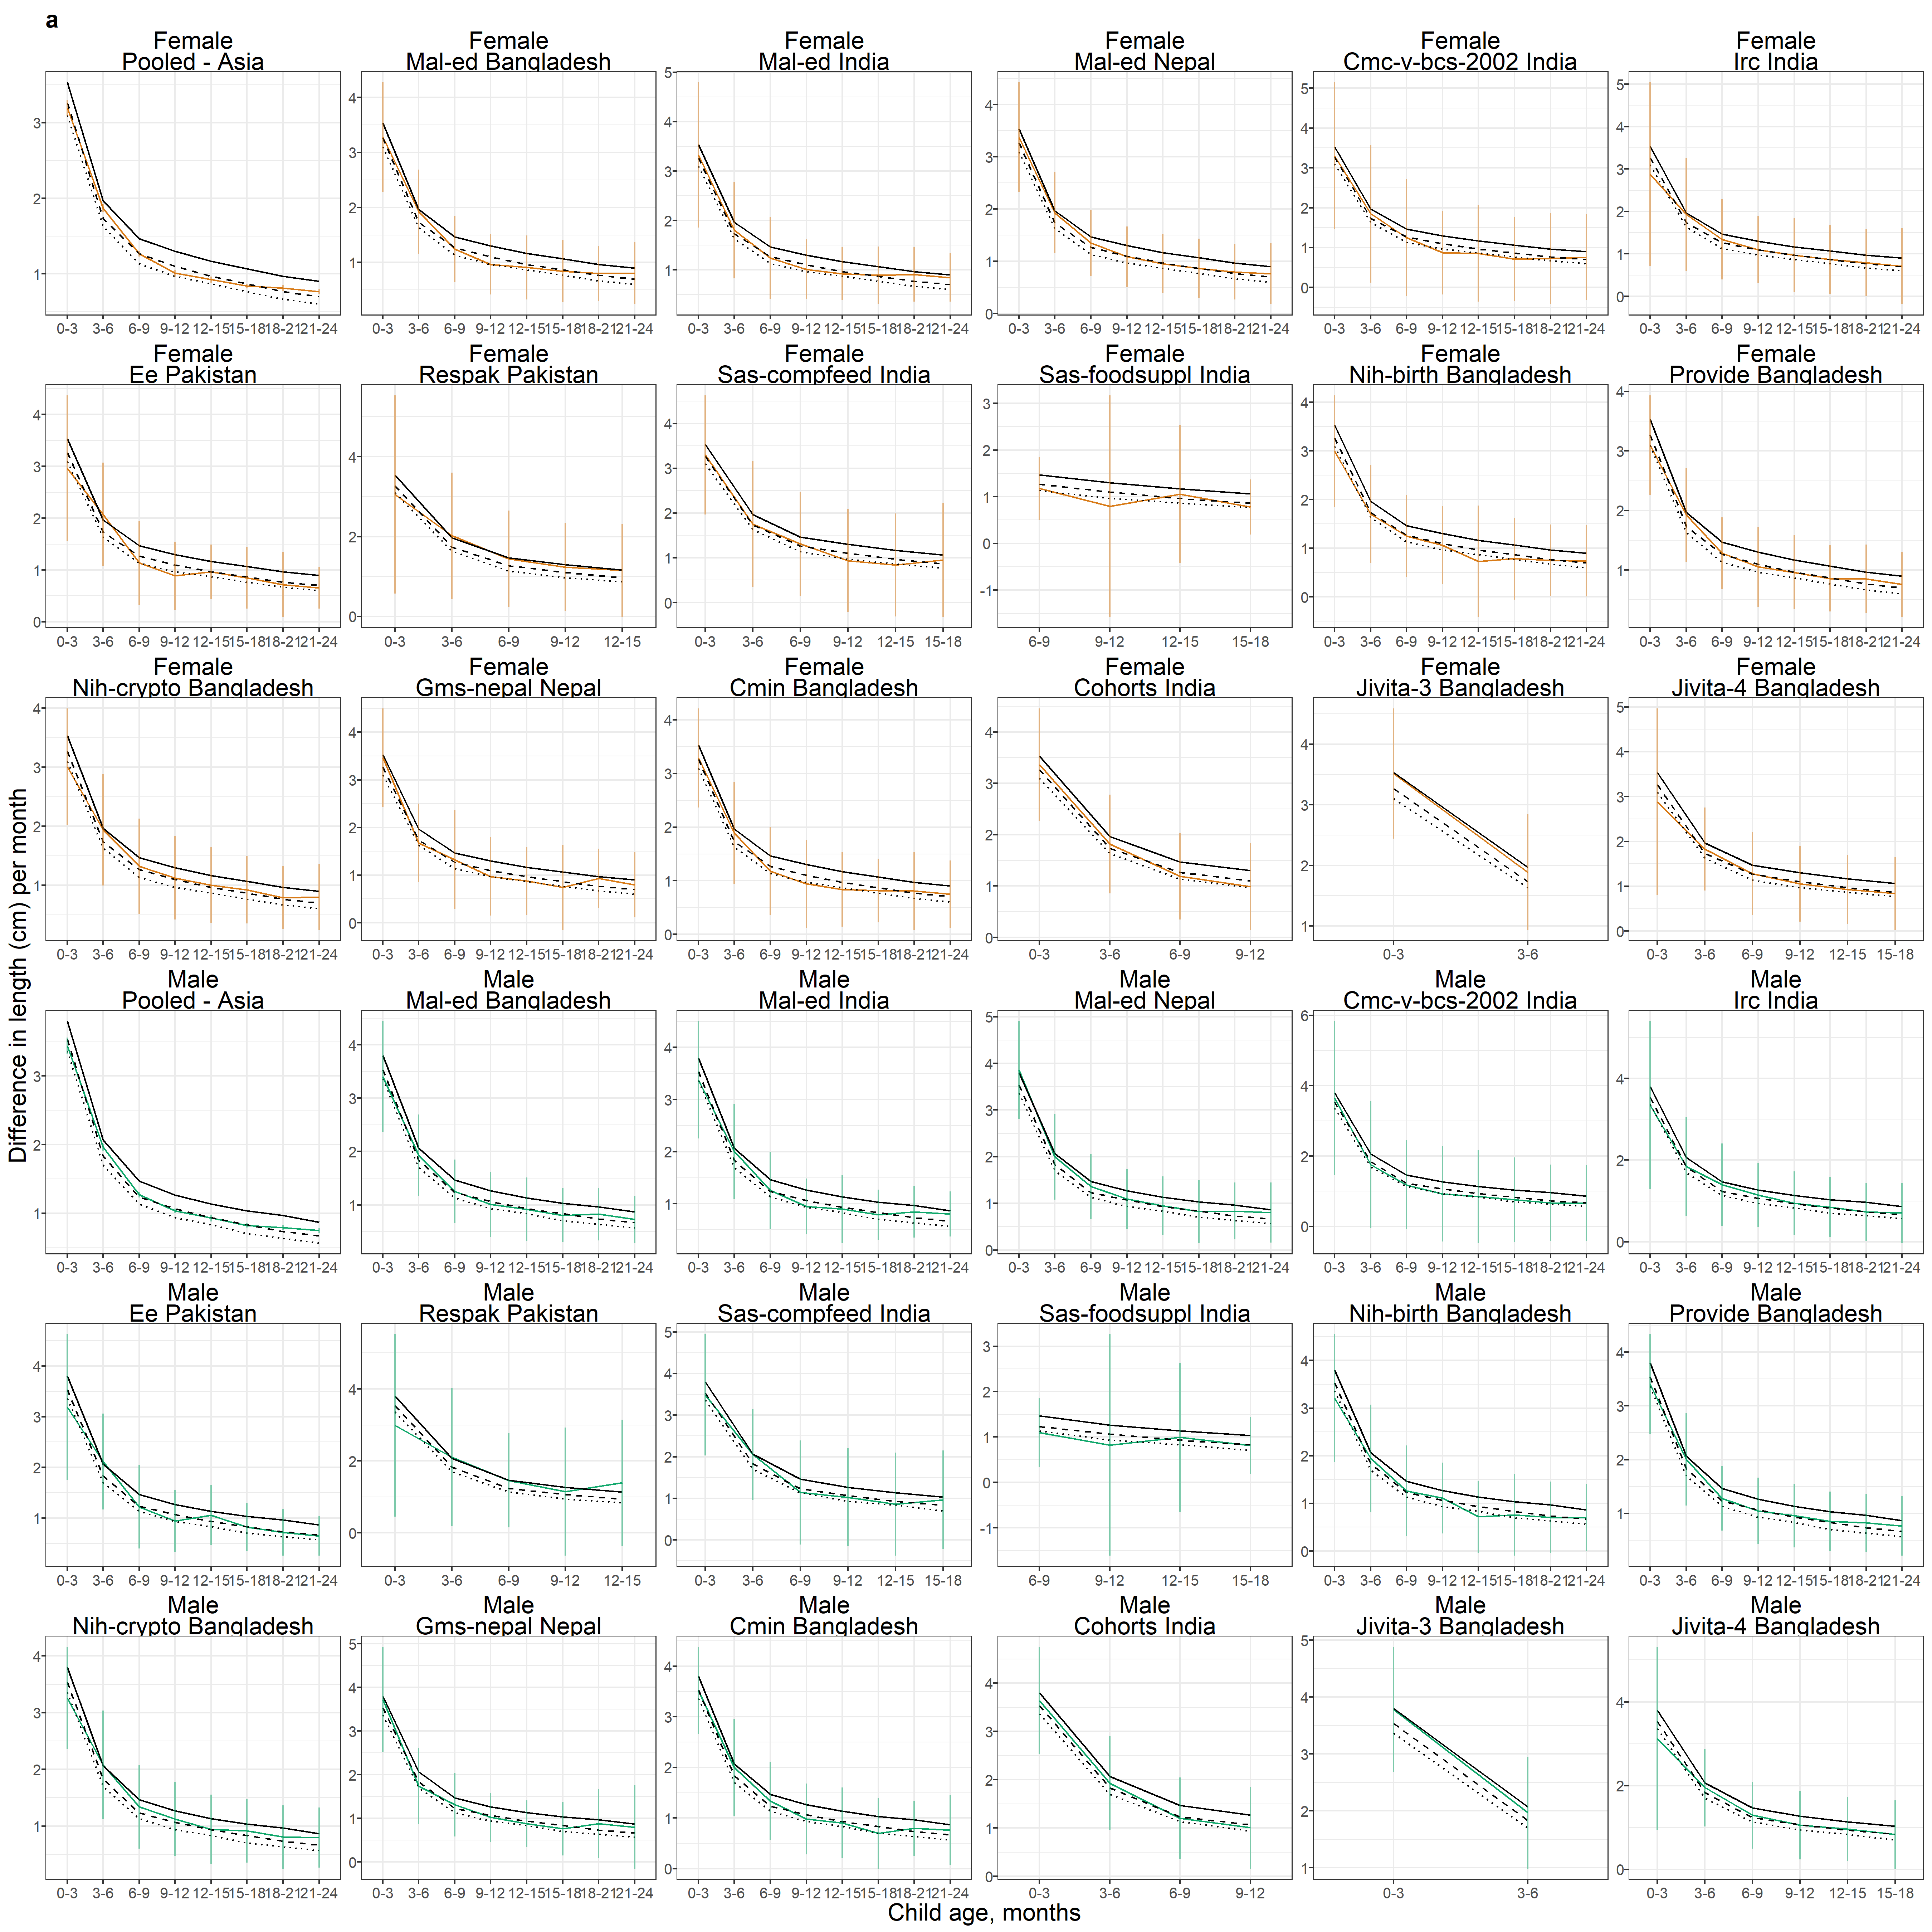
\includegraphics[width=75in]{C:/Users/andre/Documents/HBGDki/stunting/ki-longitudinal-manuscripts/figures/stunting/fig-length-2-length_vel-cohort-asia-allage-primary}

\section{LAZ velocity by age and sex}\label{laz-velocity-by-age-and-sex}

\subsection{Africa}\label{africa-4}

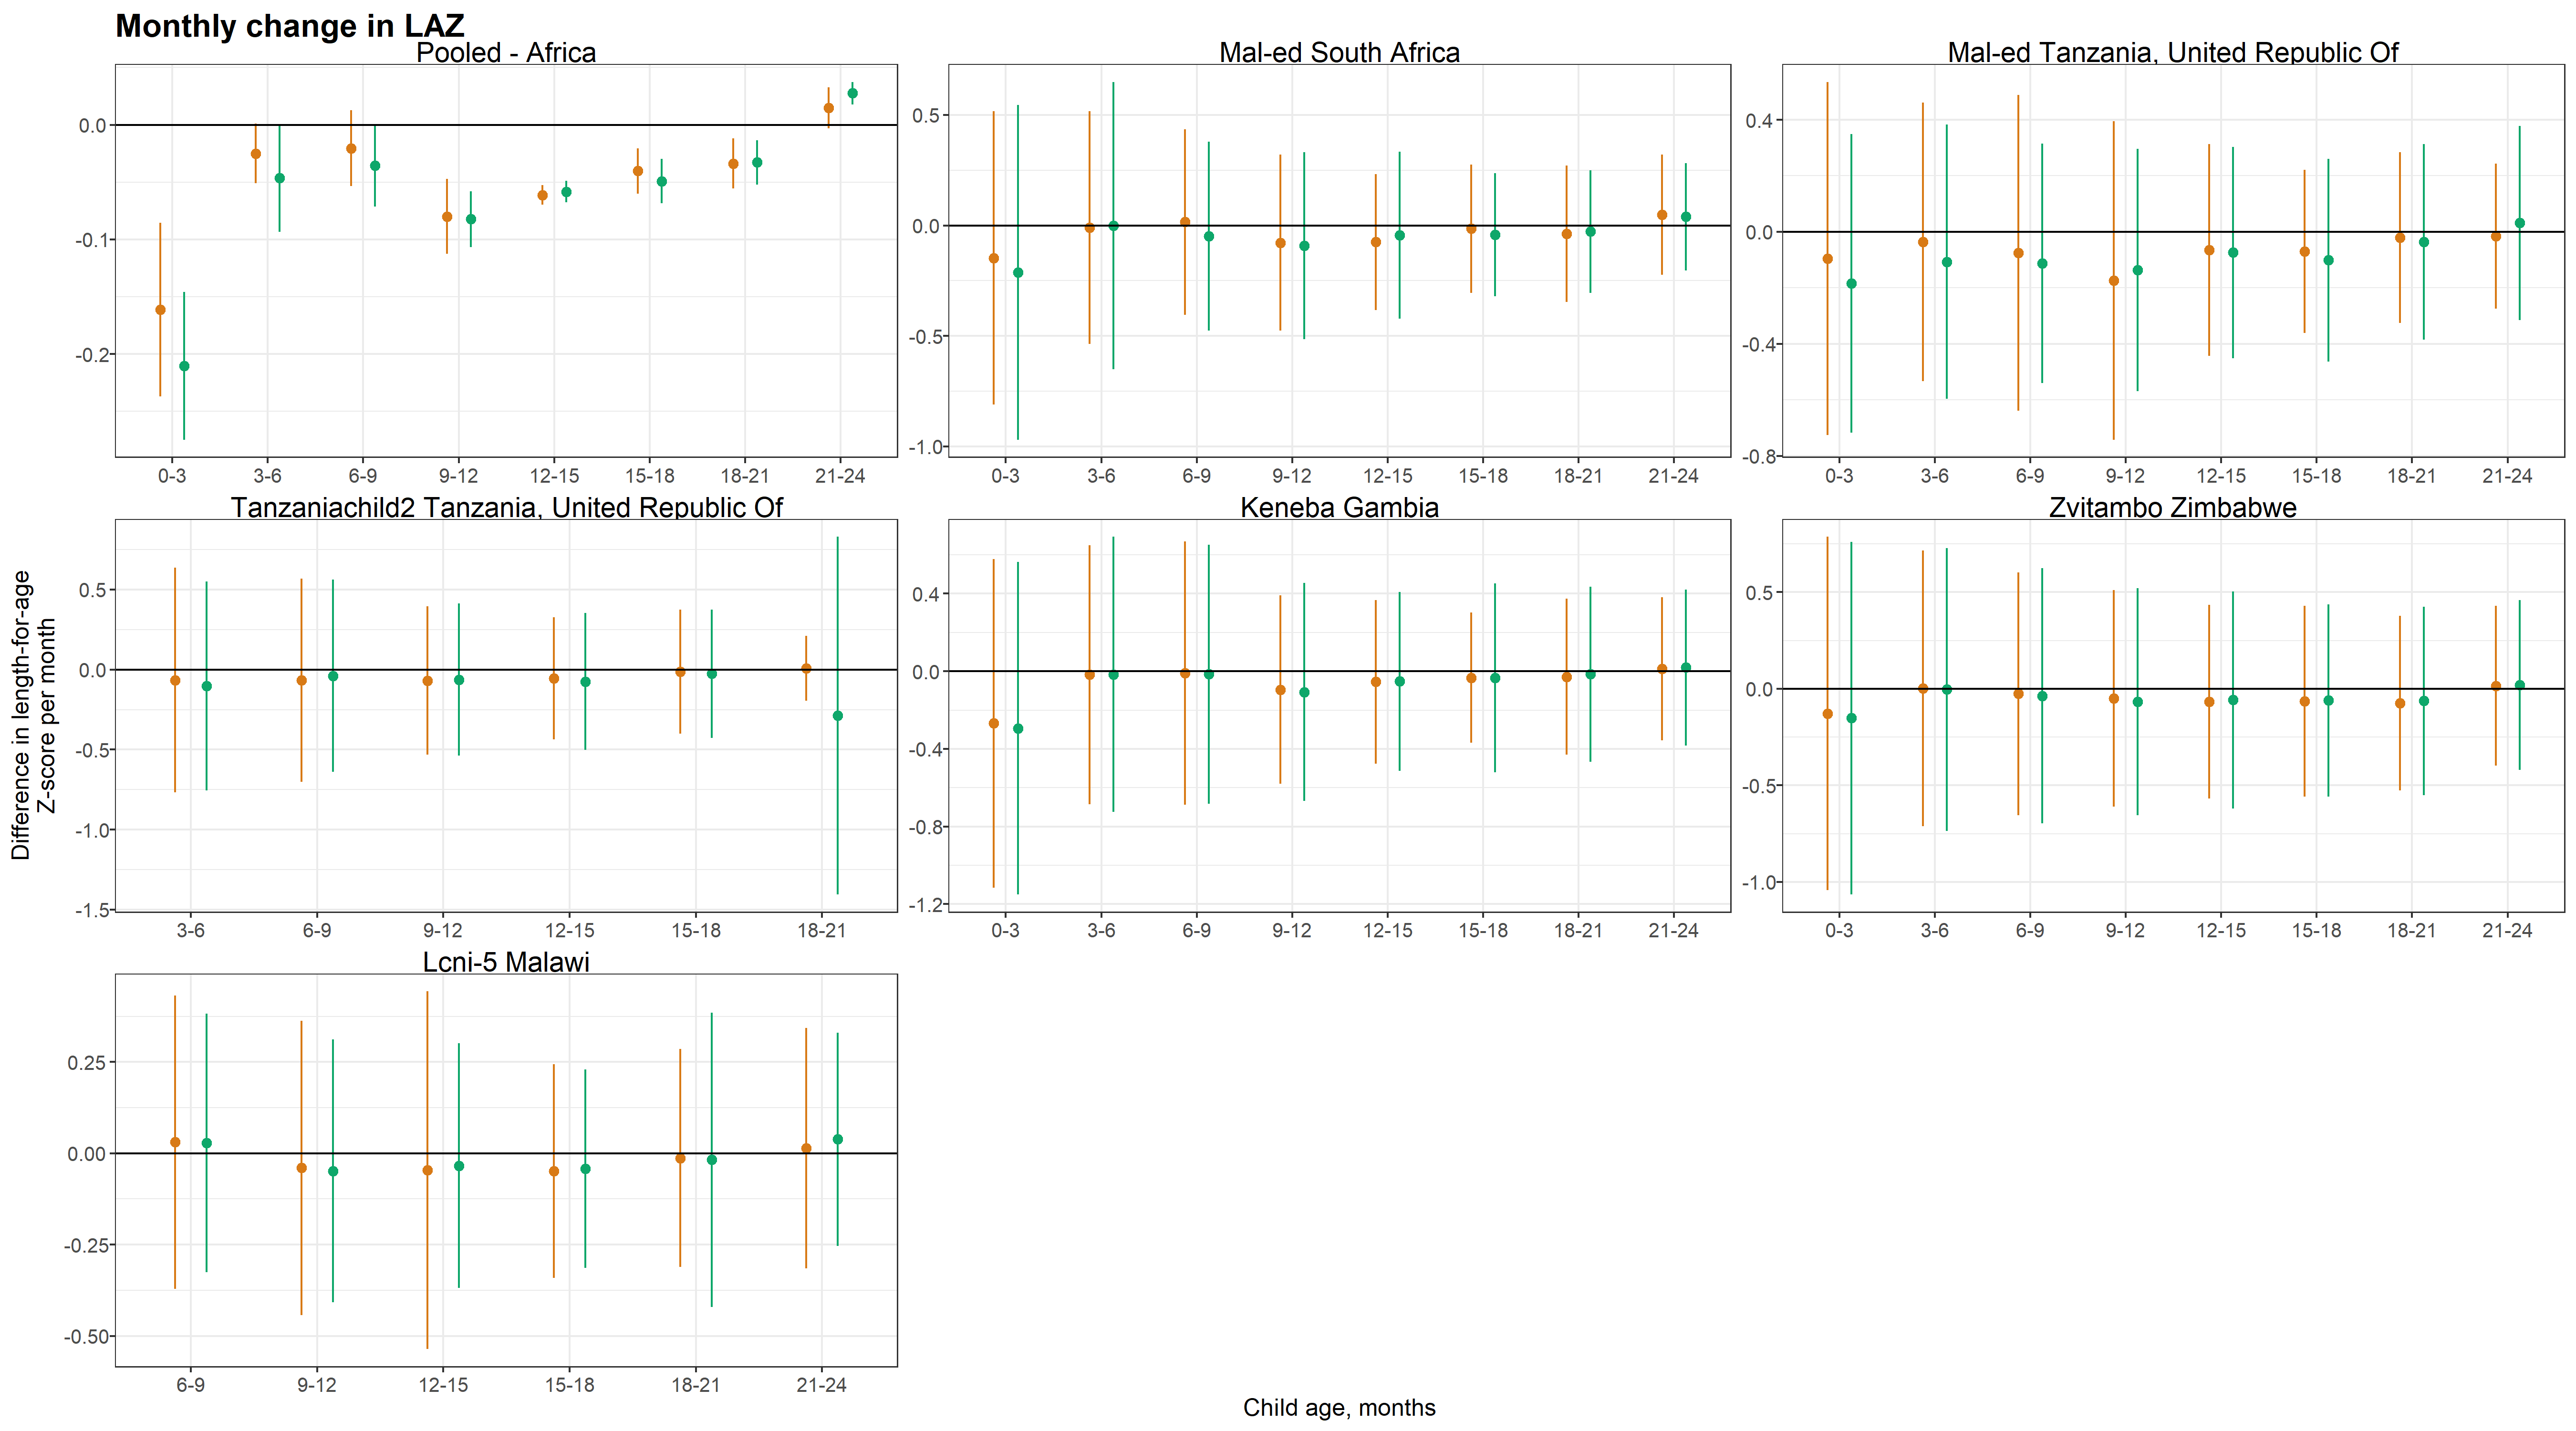
\includegraphics[width=75in]{C:/Users/andre/Documents/HBGDki/stunting/ki-longitudinal-manuscripts/figures/stunting/fig-laz-2-laz_vel-cohort-africa-allage-primary}

\subsection{Latin America}\label{latin-america-4}

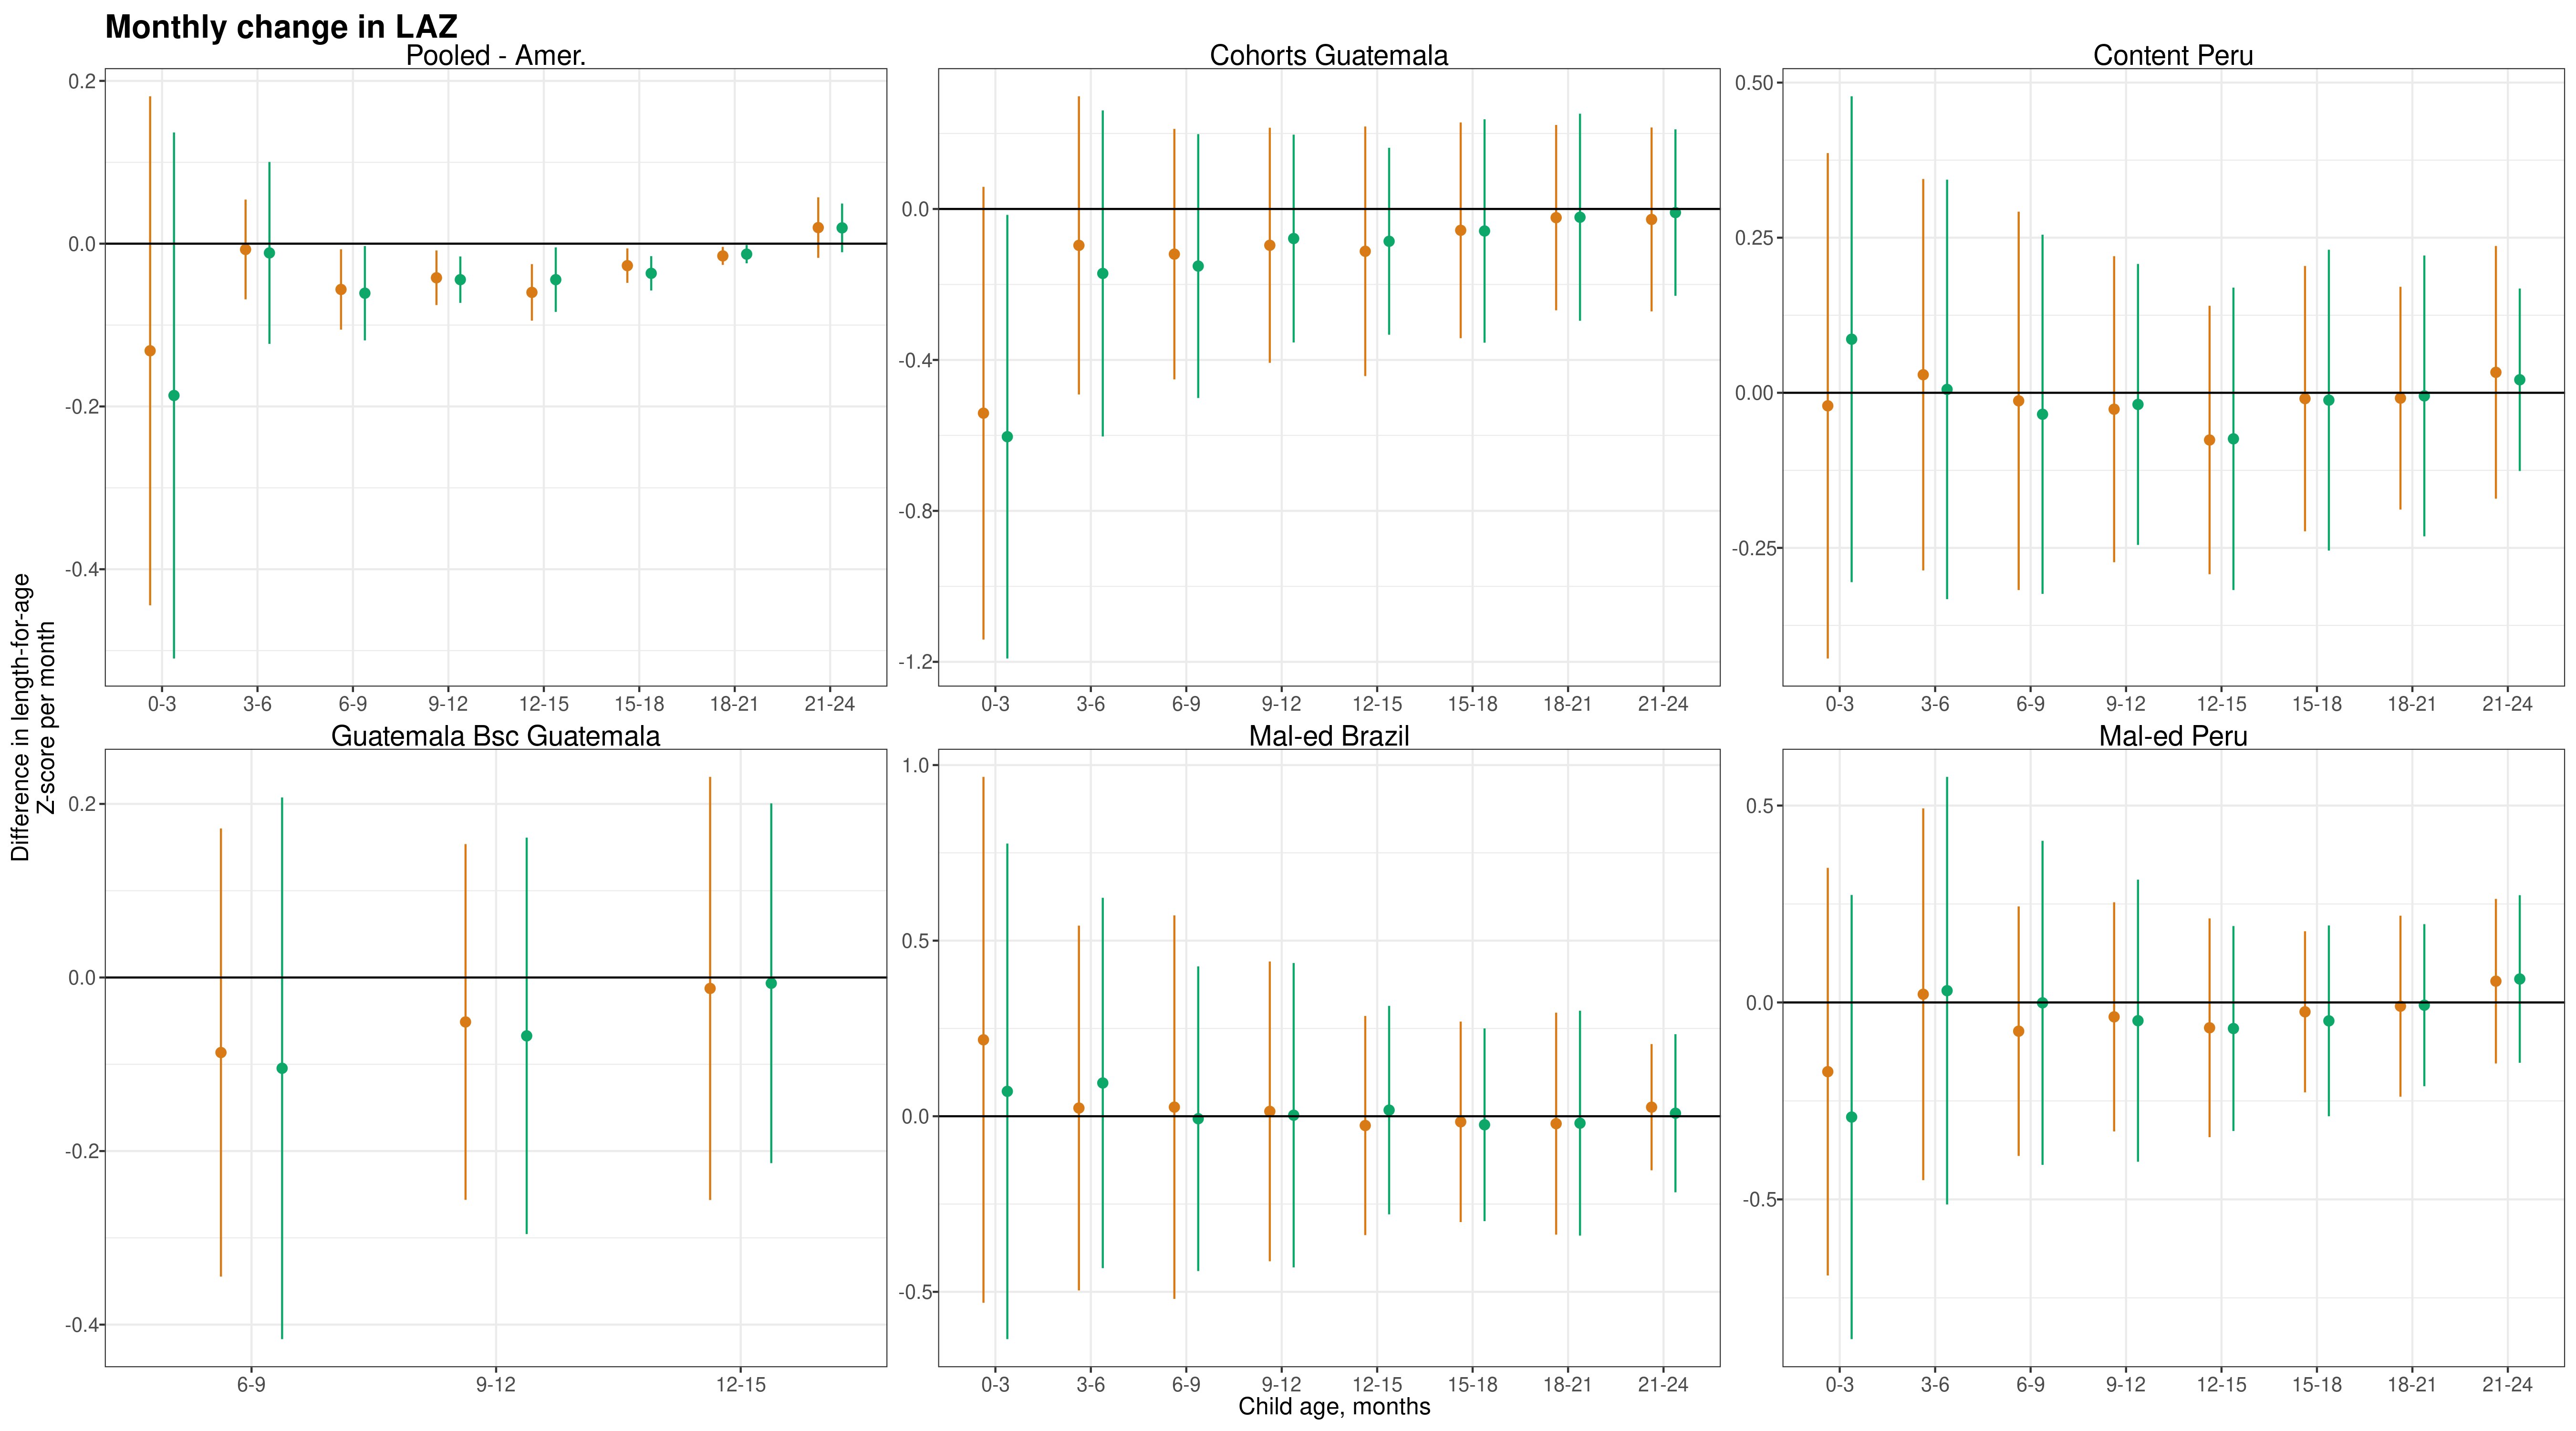
\includegraphics[width=75in]{C:/Users/andre/Documents/HBGDki/stunting/ki-longitudinal-manuscripts/figures/stunting/fig-laz-2-laz_vel-cohort-latamer-allage-primary}

\subsection{South Asia}\label{south-asia-4}

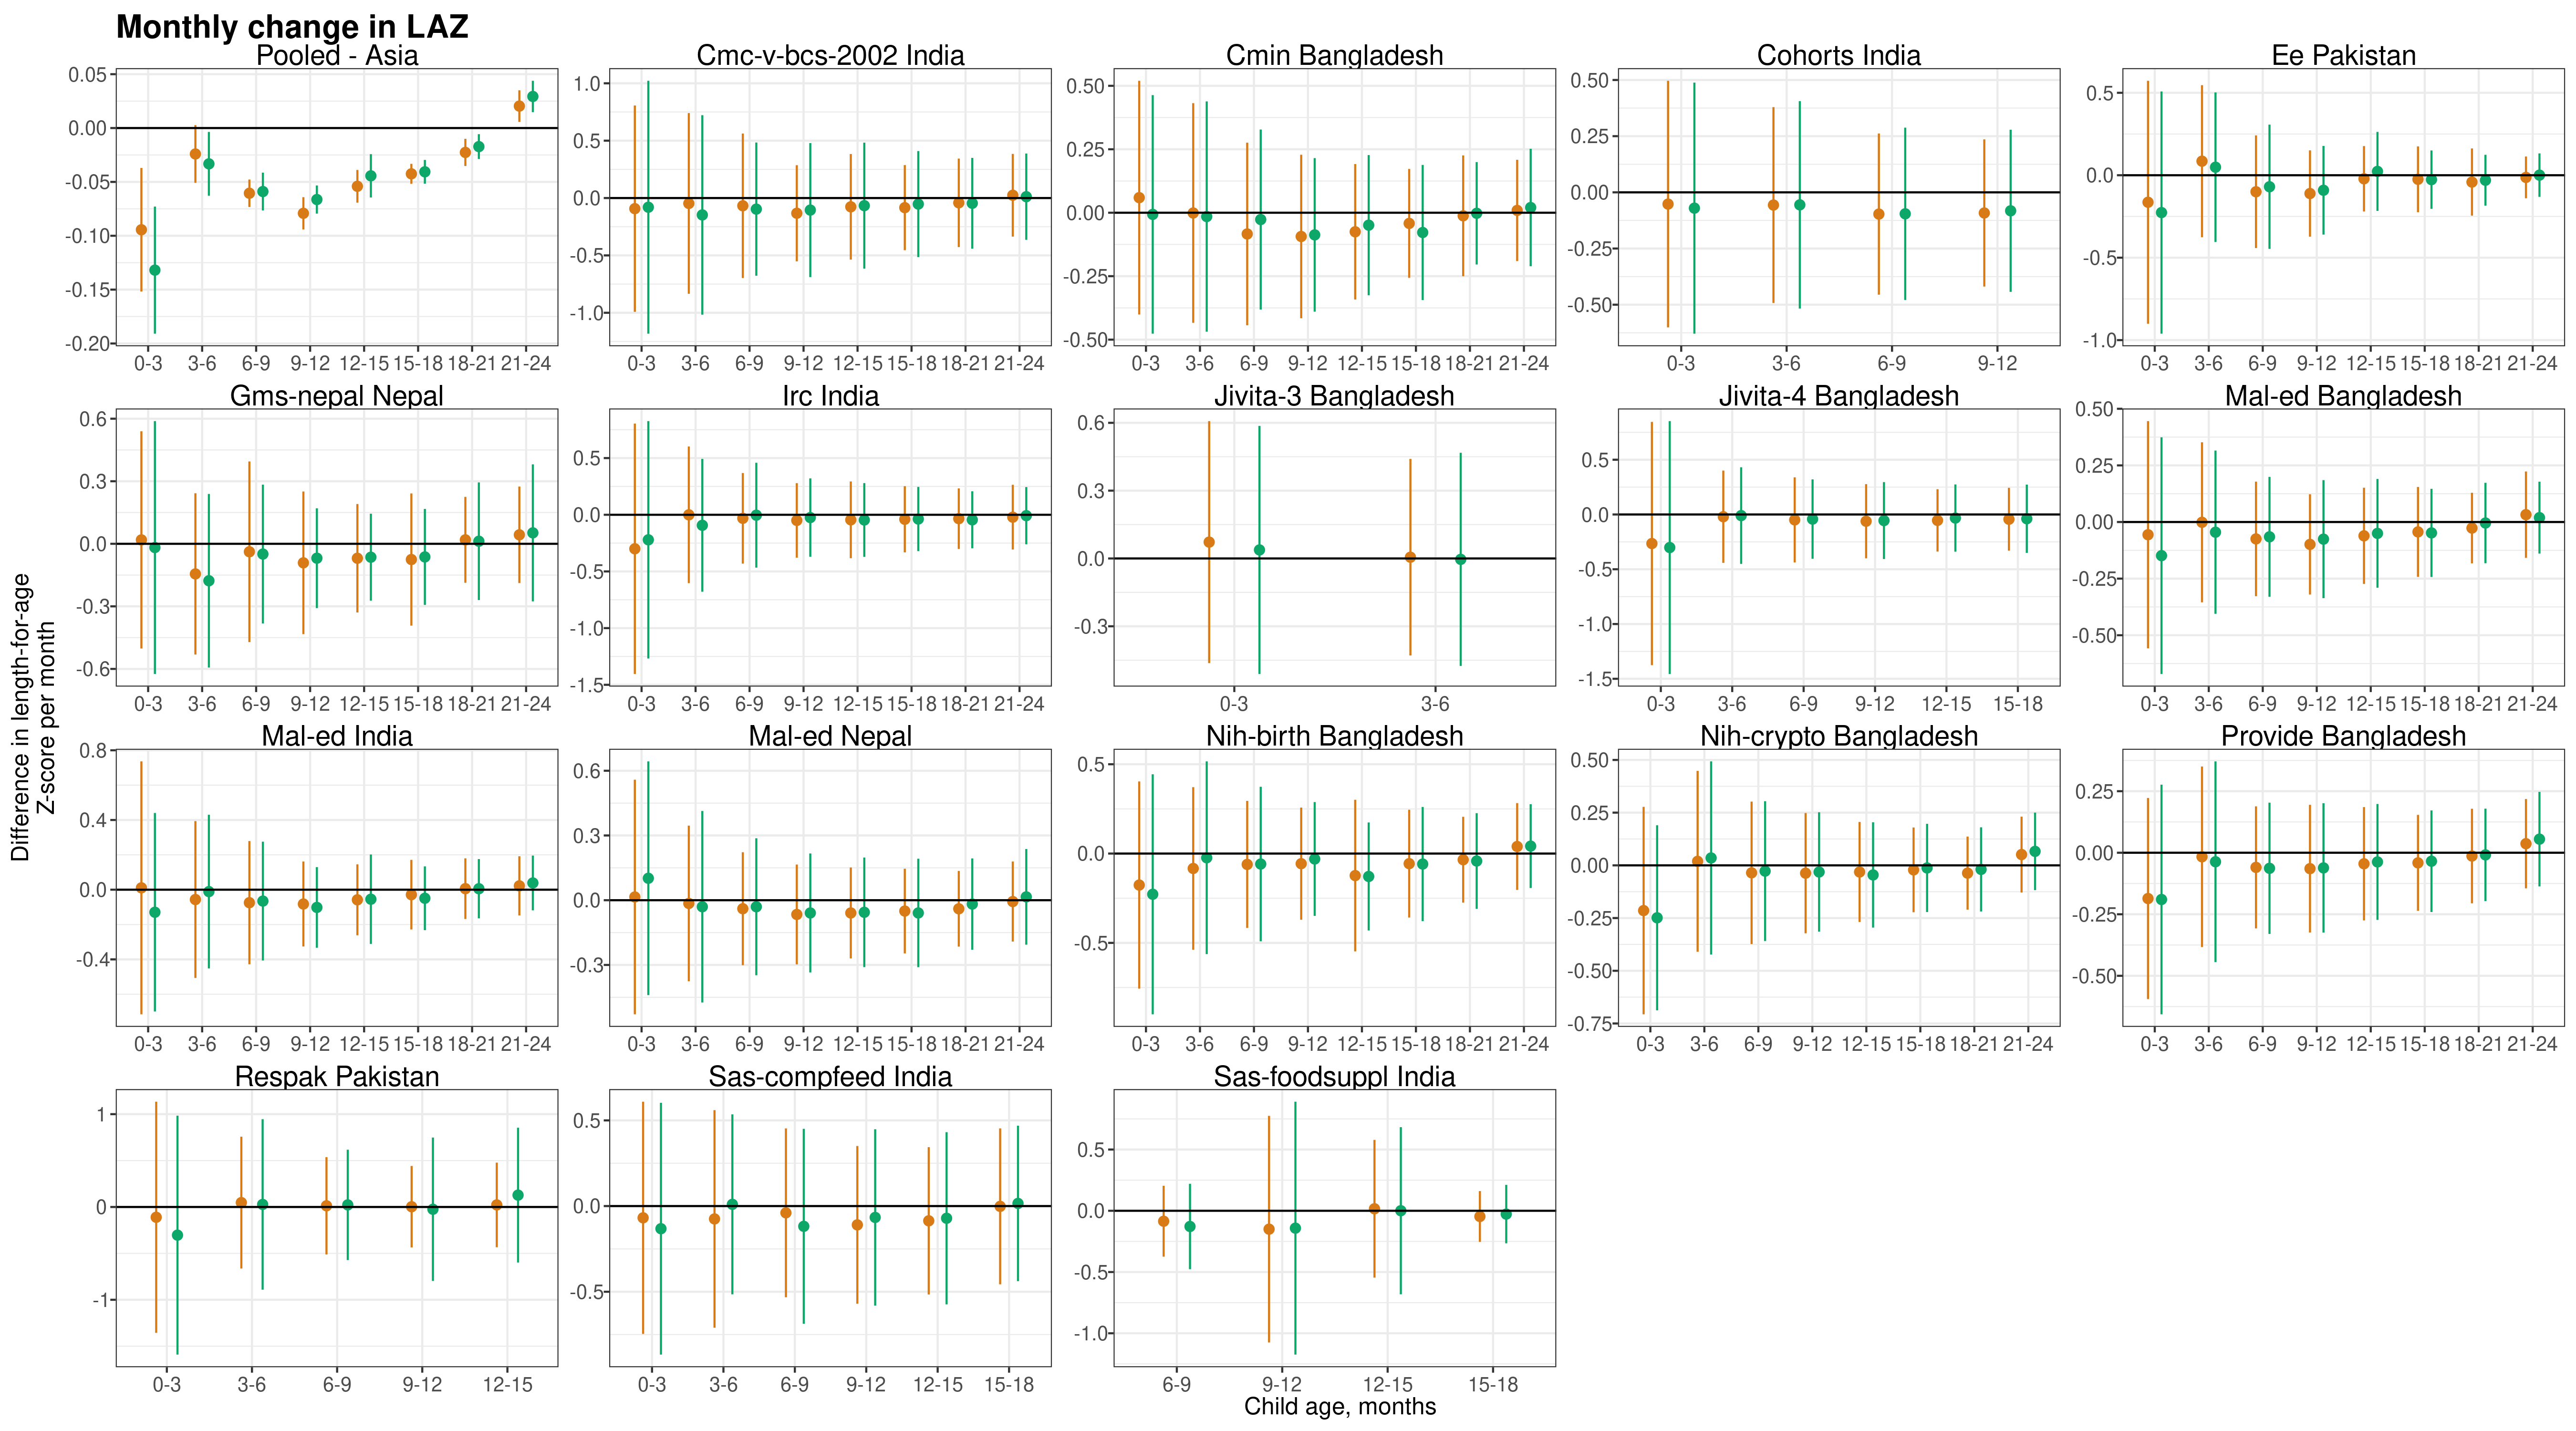
\includegraphics[width=75in]{C:/Users/andre/Documents/HBGDki/stunting/ki-longitudinal-manuscripts/figures/stunting/fig-laz-2-laz_vel-cohort-asia-allage-primary}

\chapter{Primary analyses excluding the PROBIT
study}\label{exclude-PROBIT}

\raggedright

Only one cohort from Europe met the inclusion criteria for this study --
the PROBIT study. To assess whether inclusion of this study altered our
overall study inference, we repeated analyses excluding the PROBIT
cohort, as shown below in the ``Overall'' panels. Results were very
similar with and without the PROBIT cohort. Stunting prevalence and
incidence were slightly higher at birth when excluding PROBIT, but
overall age-specific patterns remained the same. For this reason, we
chose to retain PROBIT in the primary analyses presented in this
manuscript.

\section{Mean length-for-age Z-score by
age}\label{mean-length-for-age-z-score-by-age-1}

\subsection{Including PROBIT}\label{including-probit}

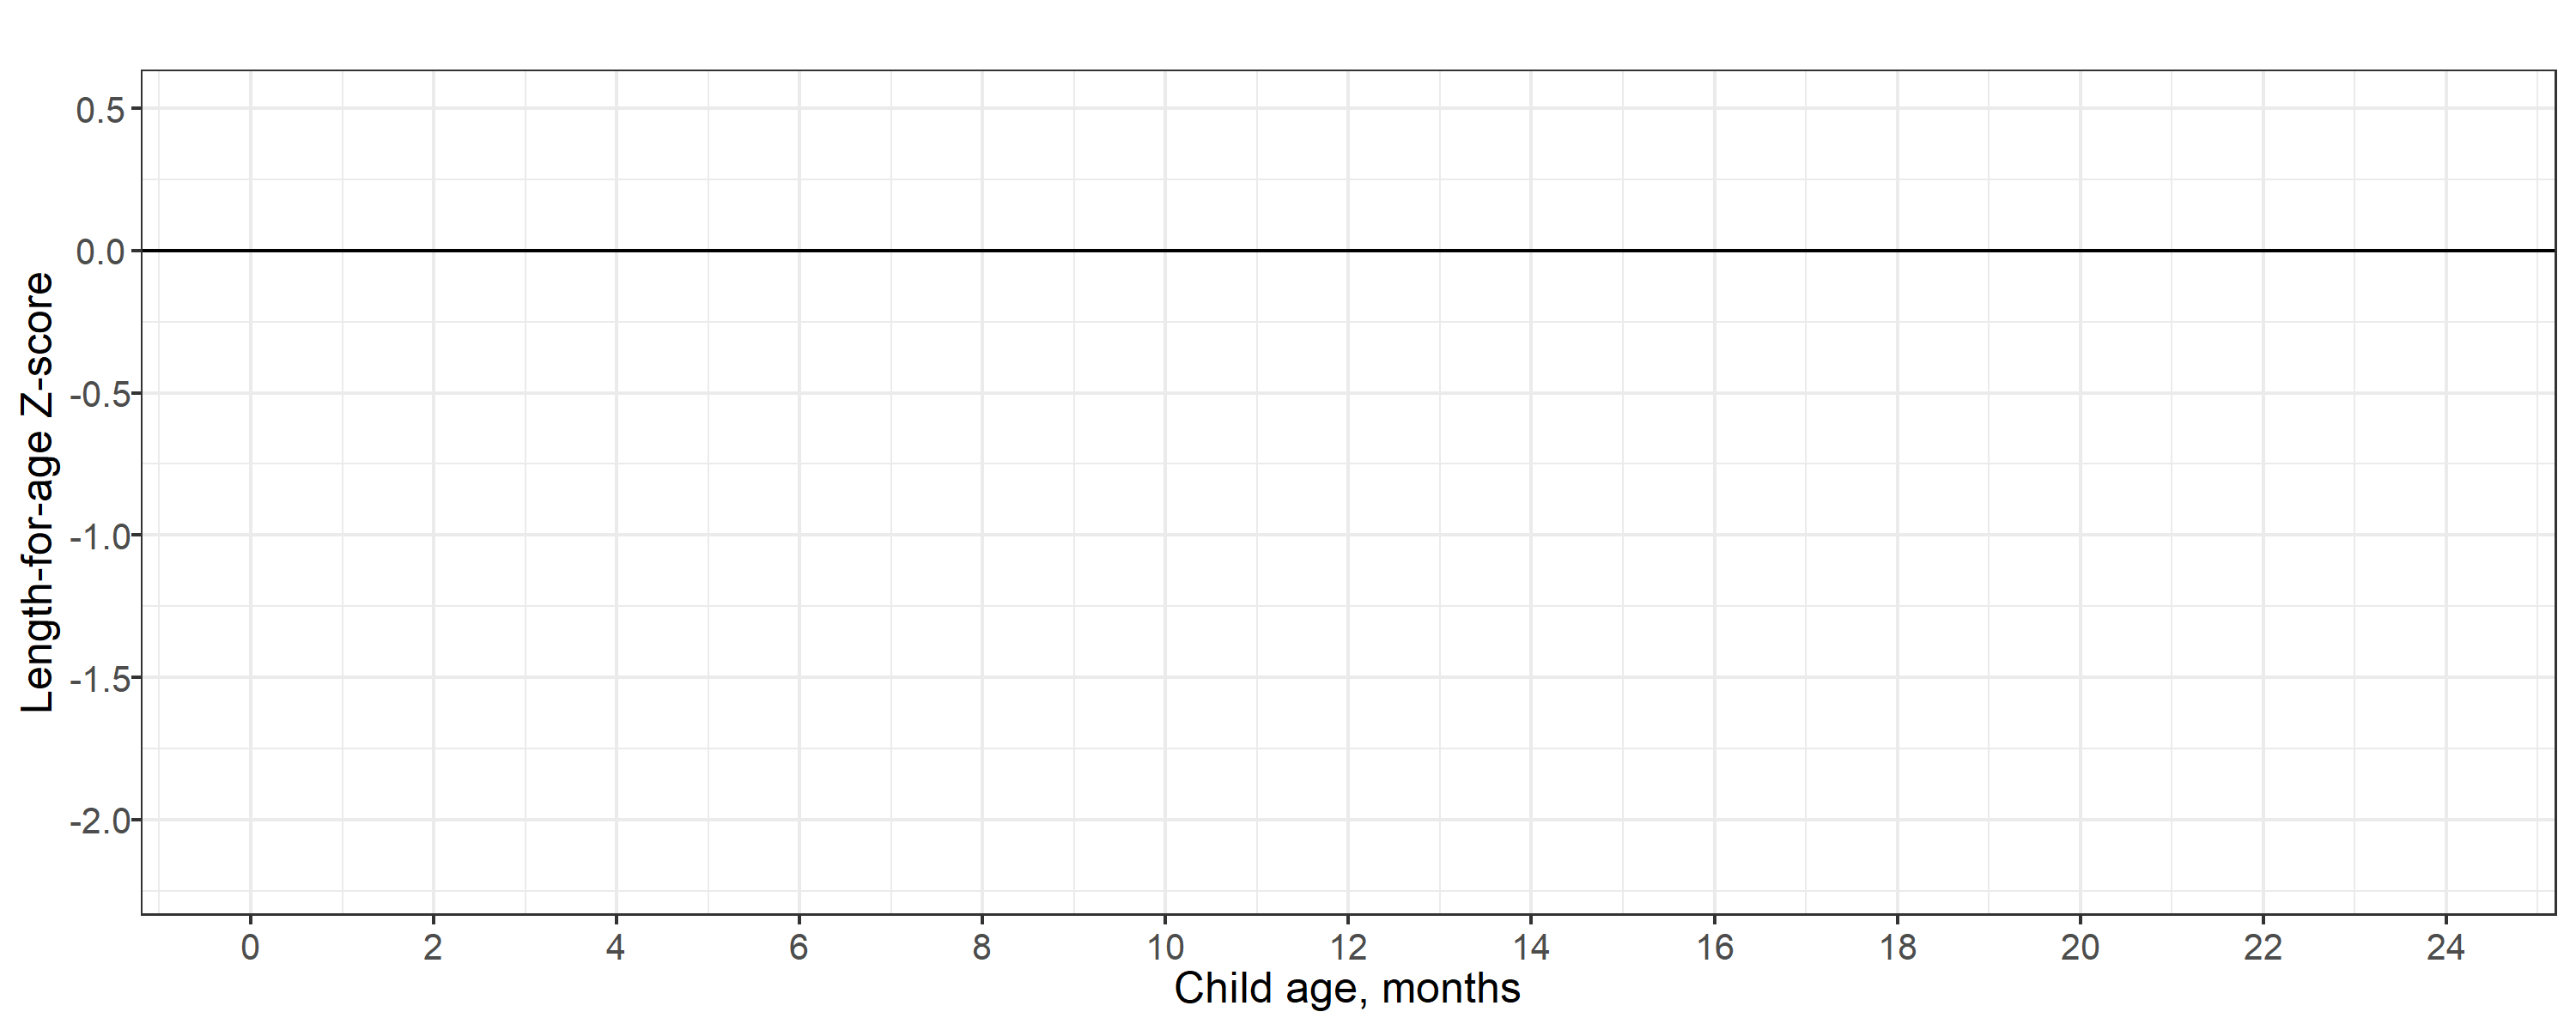
\includegraphics[width=41.67in]{C:/Users/andre/Documents/HBGDki/stunting/ki-longitudinal-manuscripts/figures/stunting/fig-laz-2-mean-overall_region--allage-primary}

\subsection{Excluding PROBIT}\label{excluding-probit}

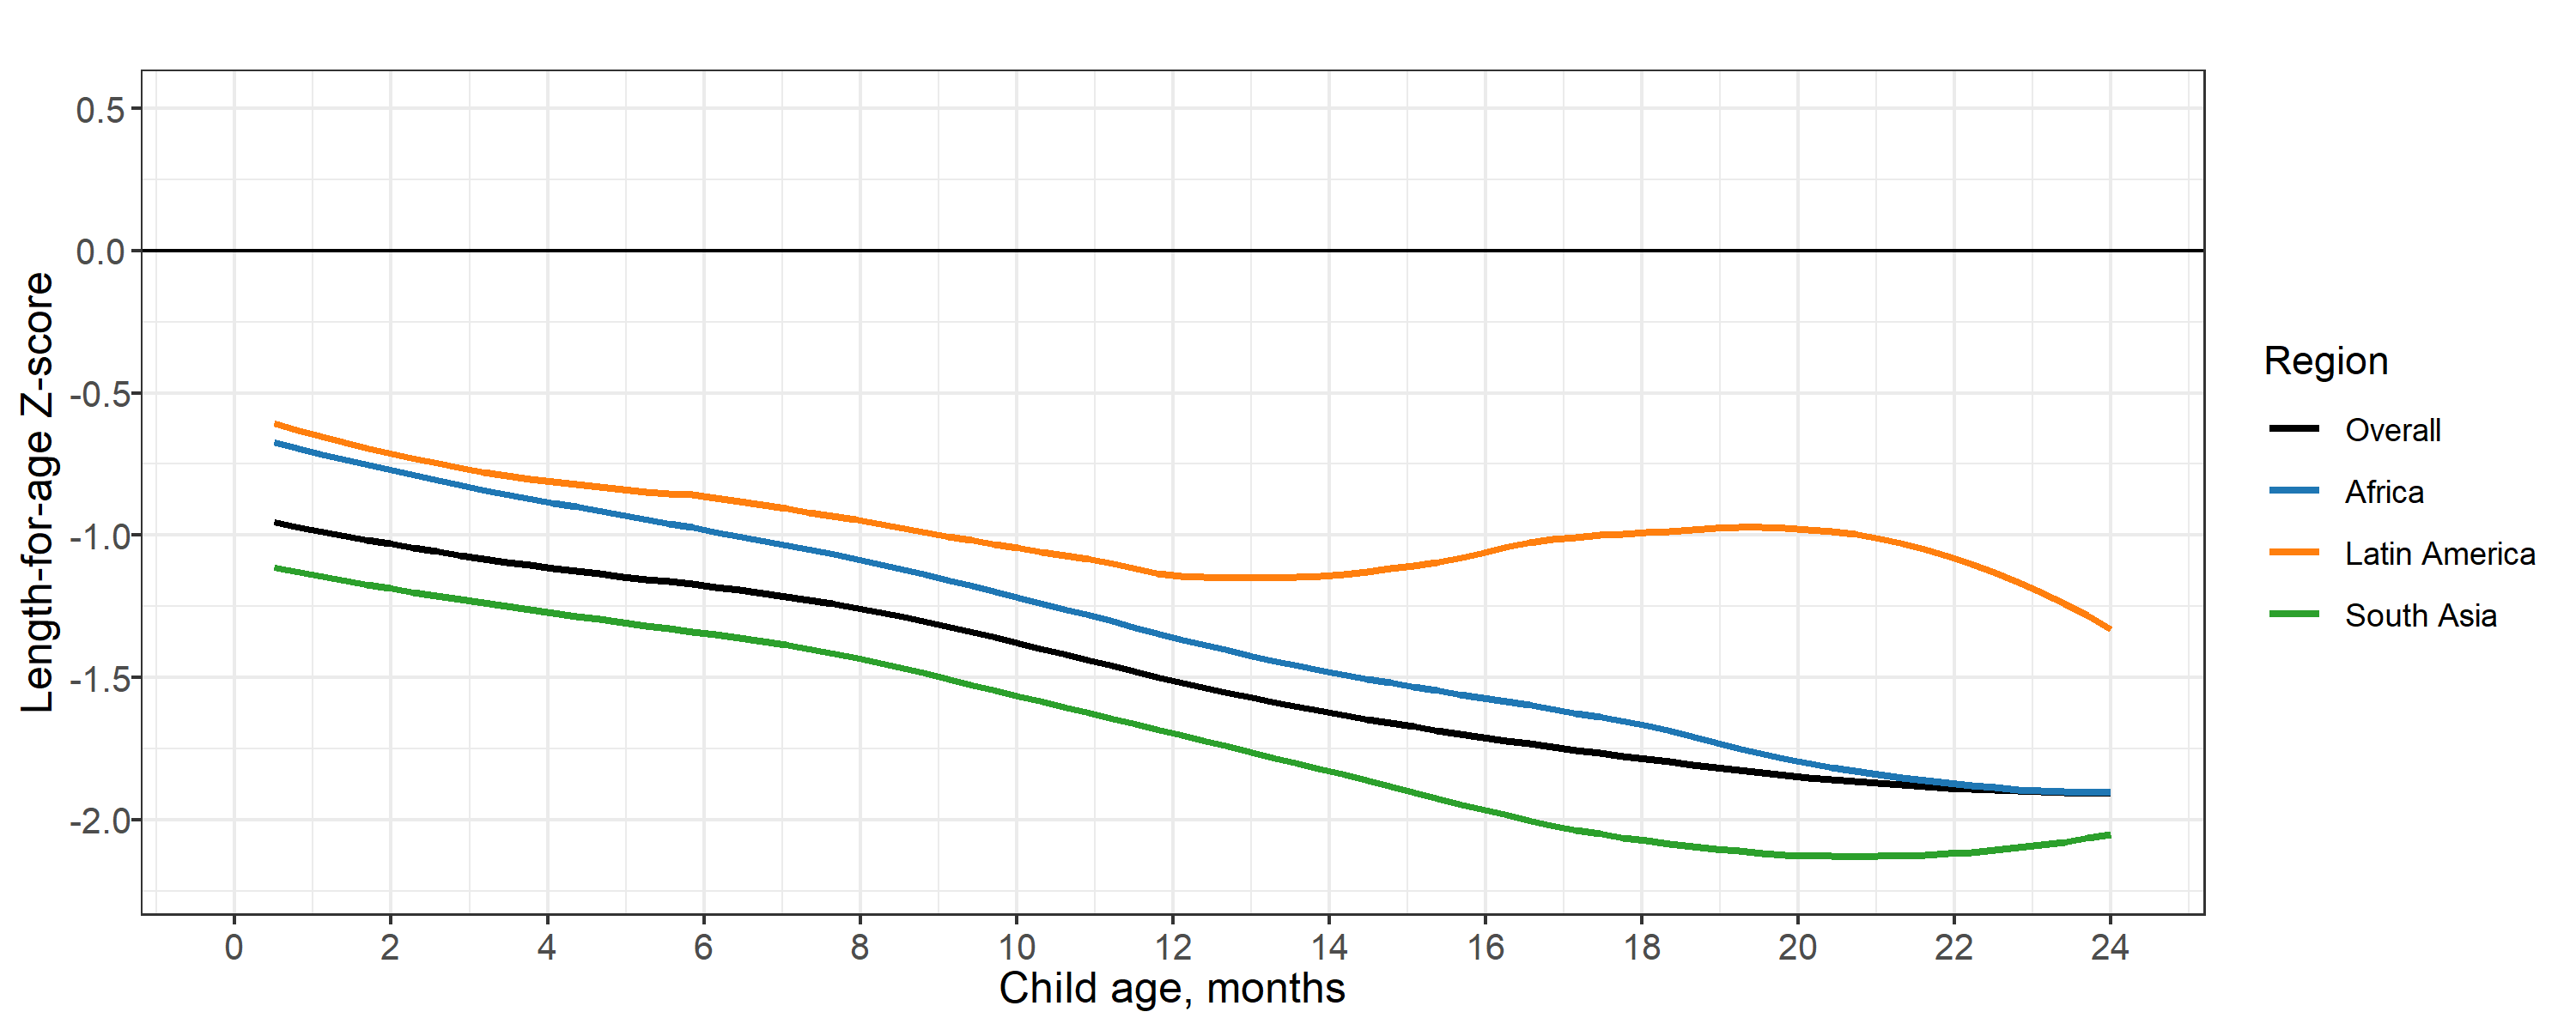
\includegraphics[width=41.67in]{C:/Users/andre/Documents/HBGDki/stunting/ki-longitudinal-manuscripts/figures/stunting/fig-laz-2-mean-overall_region--allage-primary_no_probit}

\section{Age-specific prevalence}\label{age-specific-prevalence-1}

\subsection{Including PROBIT}\label{including-probit-1}

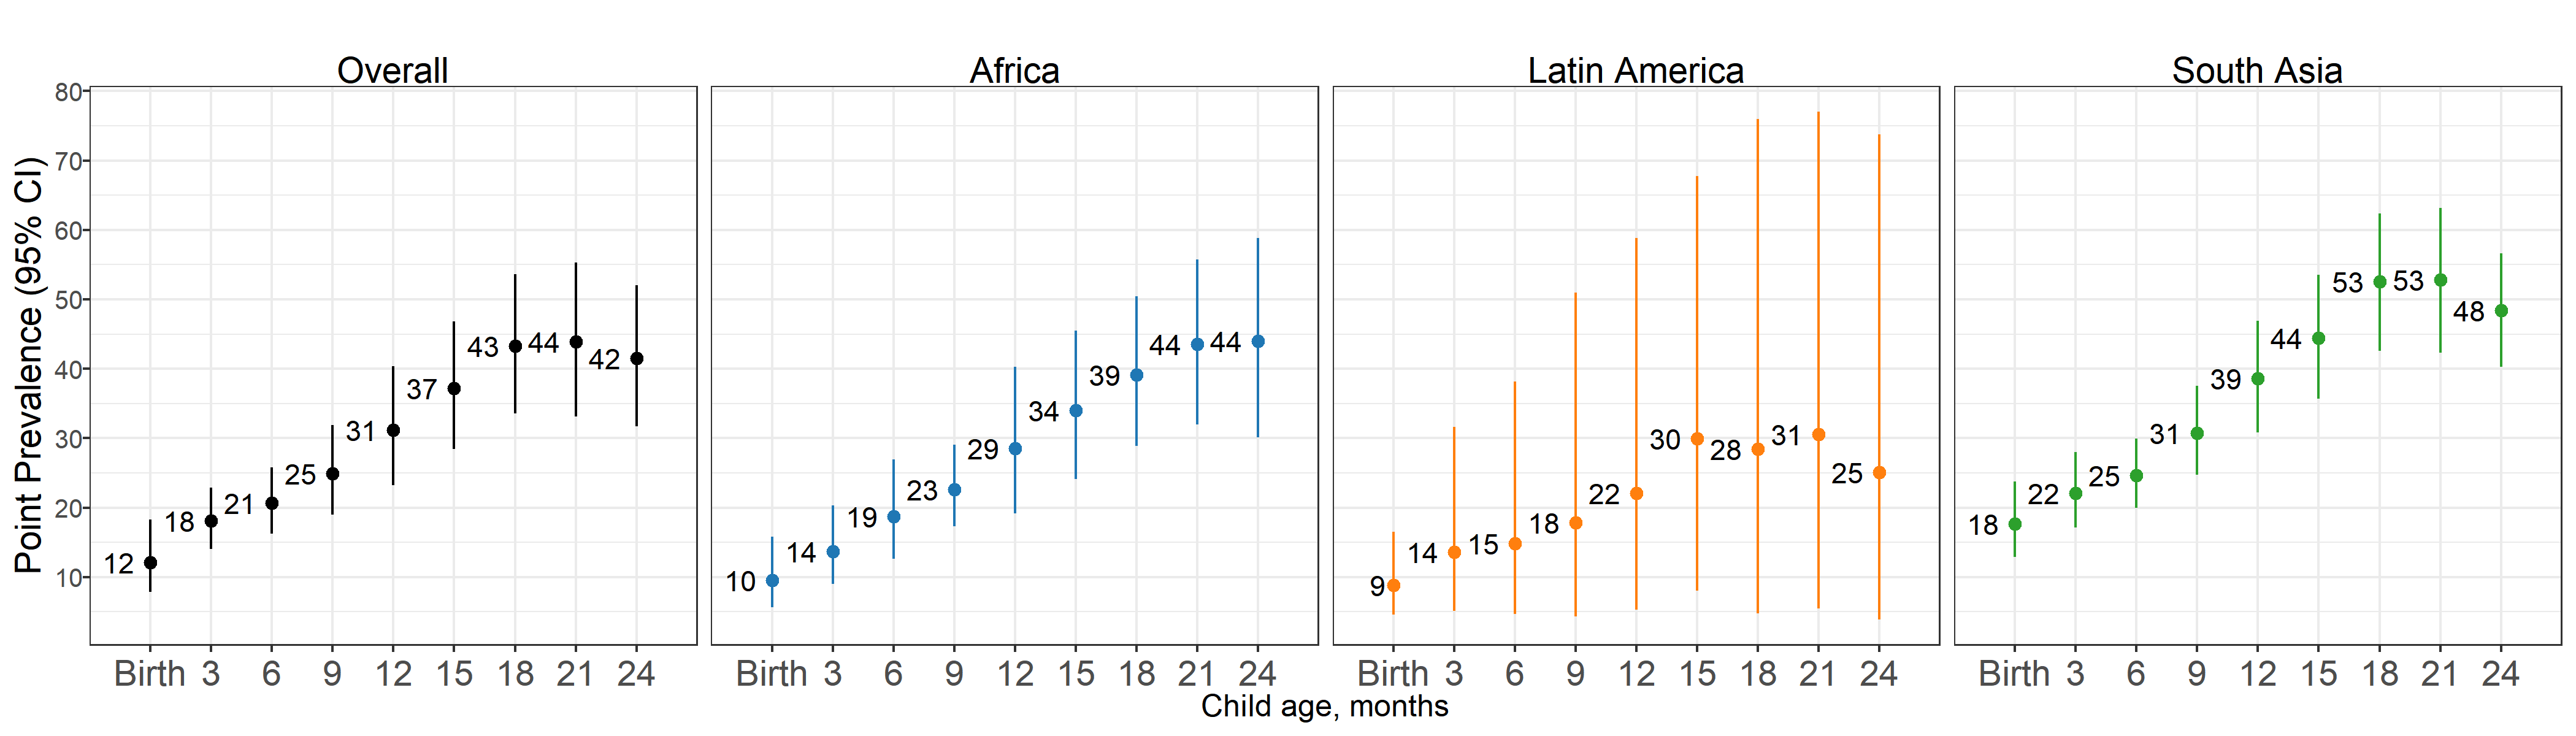
\includegraphics[width=58.33in]{C:/Users/andre/Documents/HBGDki/stunting/ki-longitudinal-manuscripts/figures/stunting/fig-stunt-2-prev-overall_region--allage-primary}

\subsection{Excluding PROBIT}\label{excluding-probit-1}

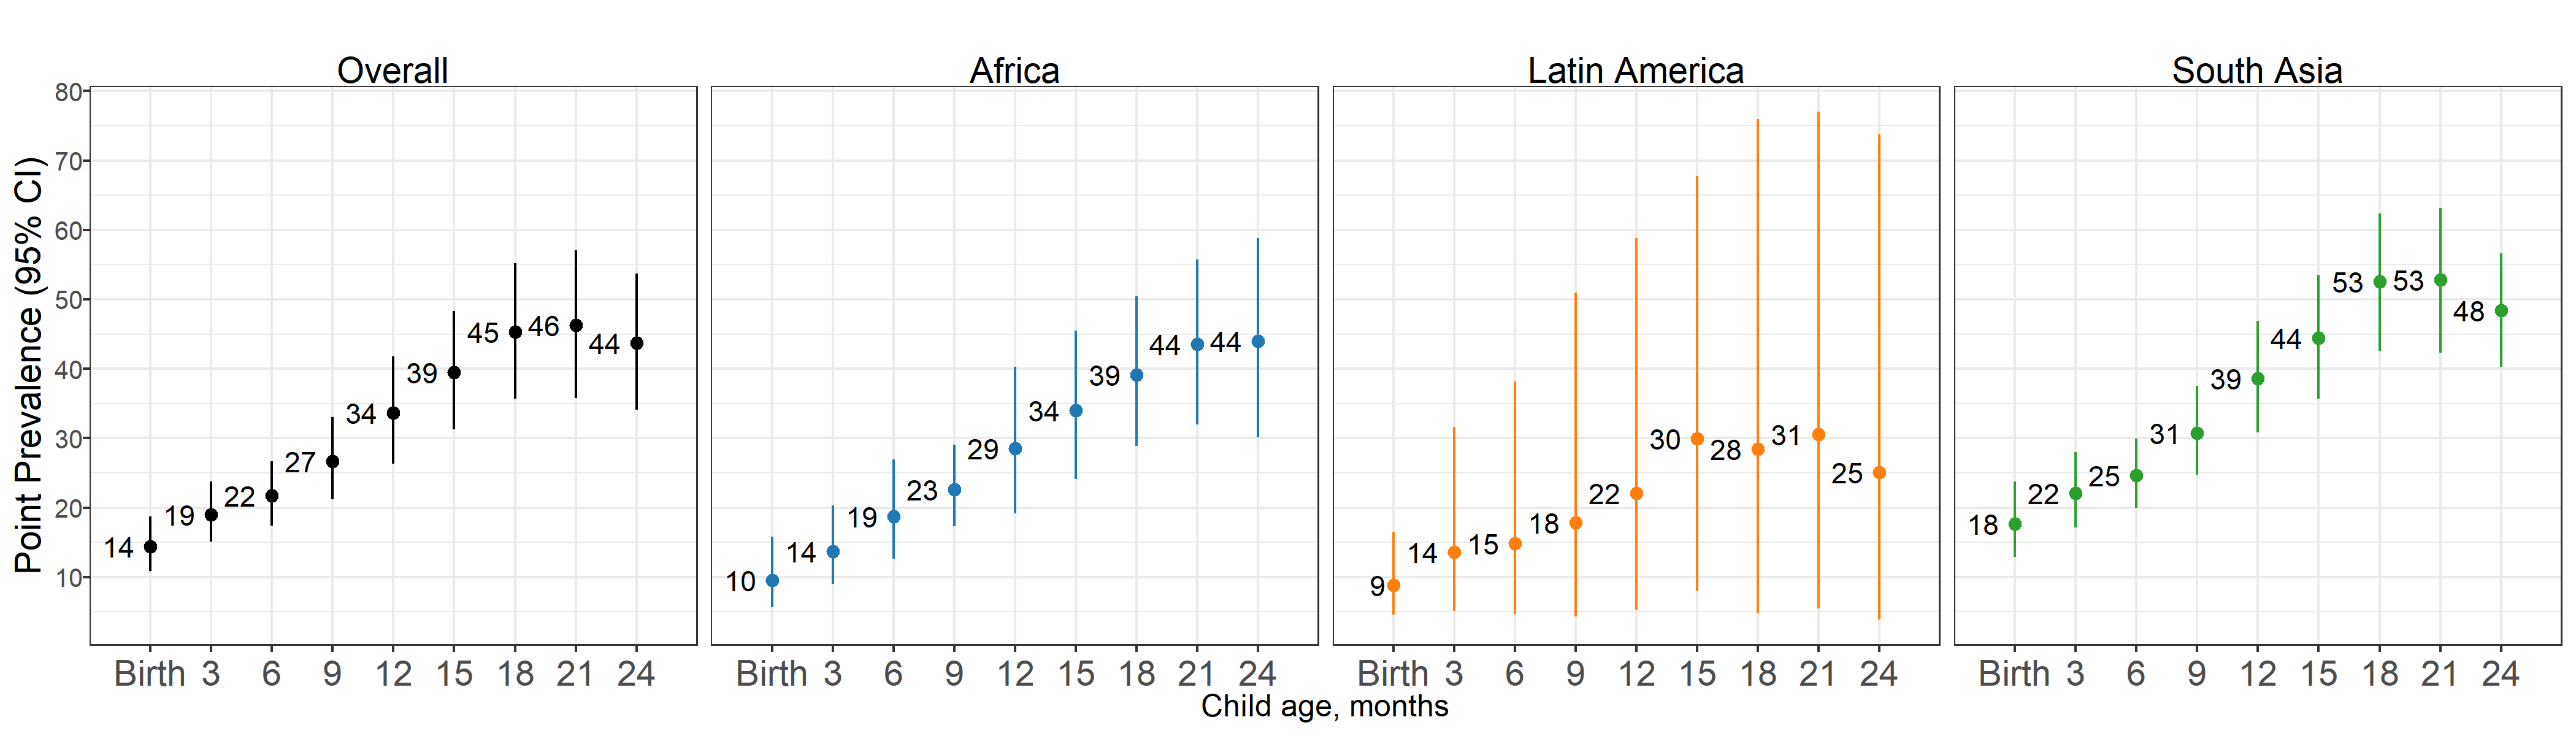
\includegraphics[width=58.33in]{C:/Users/andre/Documents/HBGDki/stunting/ki-longitudinal-manuscripts/figures/stunting/fig-stunt-2-prev-overall_region--allage-primary_no_probit}

\section{Age-specific incidence}\label{age-specific-incidence-1}

\subsection{Including PROBIT}\label{including-probit-2}

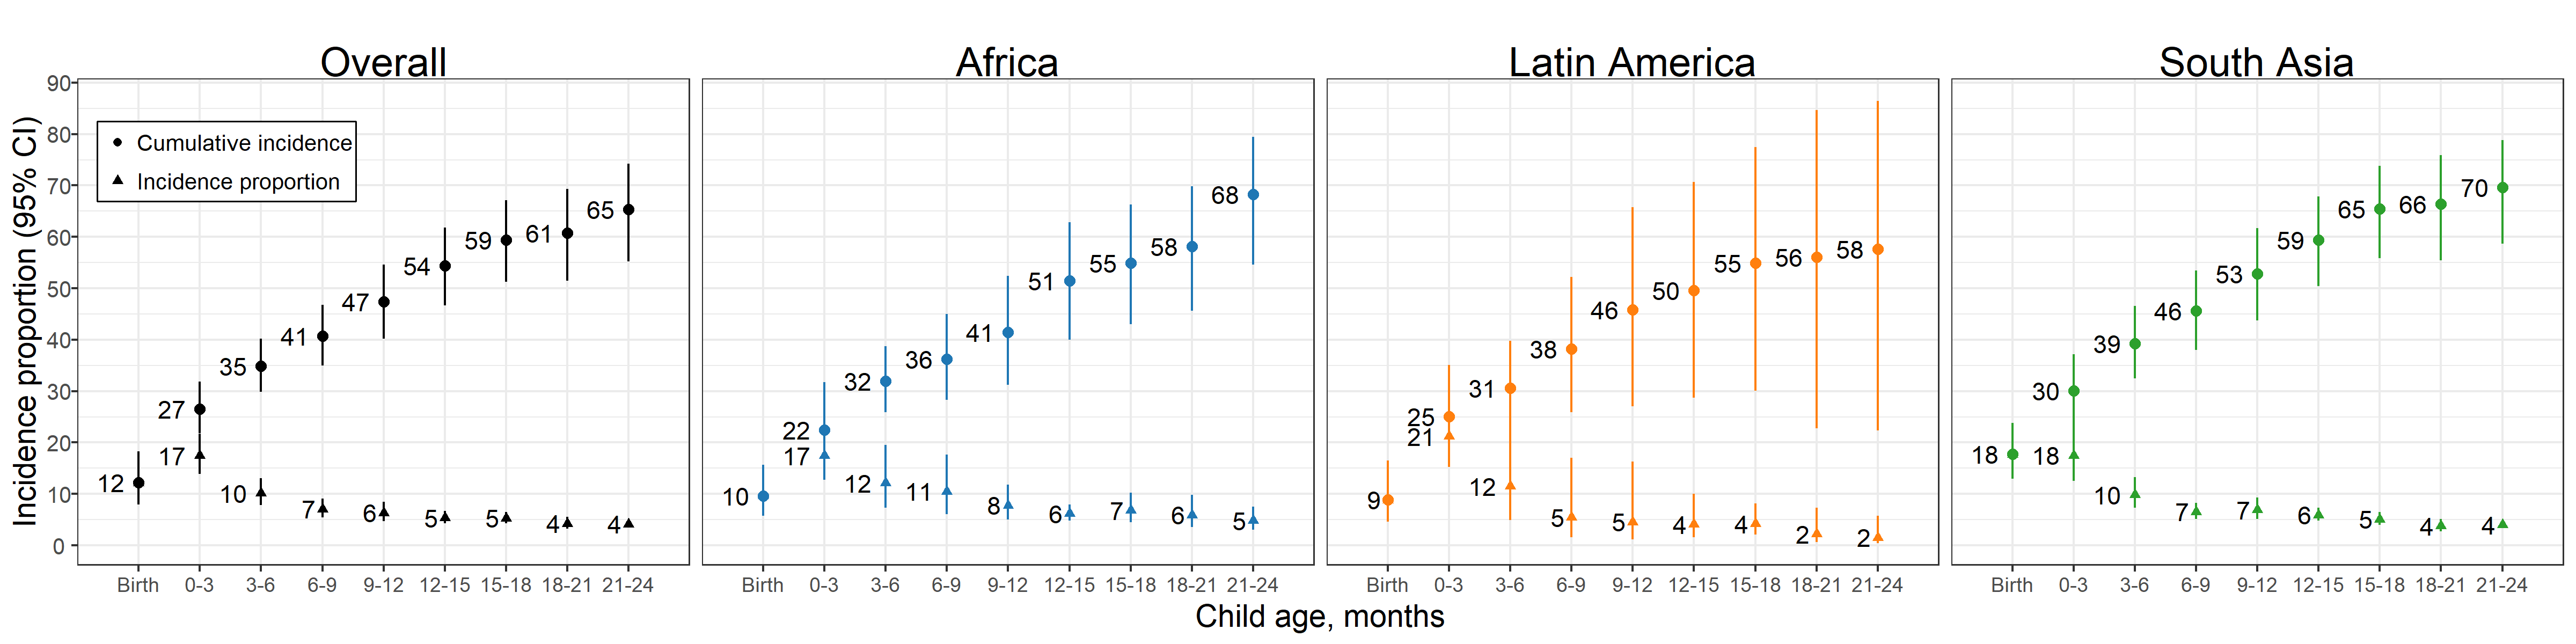
\includegraphics[width=66.67in]{C:/Users/andre/Documents/HBGDki/stunting/ki-longitudinal-manuscripts/figures/stunting/fig-stunt-2-inc-overall_region--allage-primary}

\subsection{Excluding PROBIT}\label{excluding-probit-2}

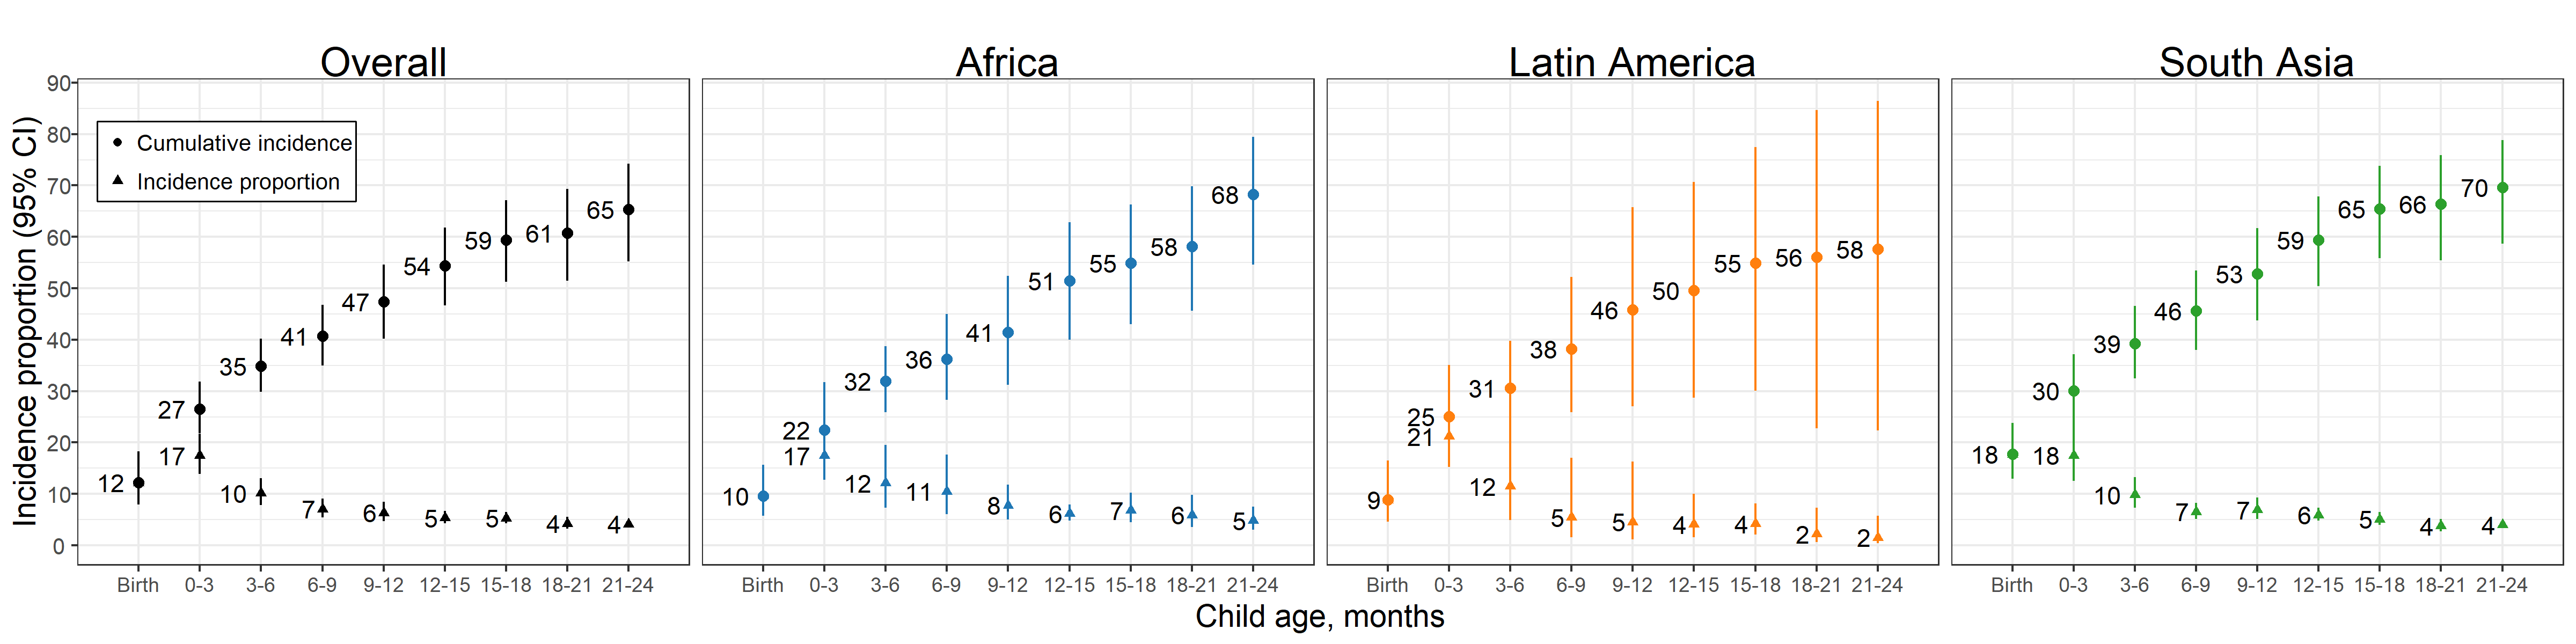
\includegraphics[width=66.67in]{C:/Users/andre/Documents/HBGDki/stunting/ki-longitudinal-manuscripts/figures/stunting/fig-stunt-2-inc-overall_region--allage-primary}

\chapter{Analysis with monthly cohorts}\label{monthly}

\raggedright

To explore the influence of differing numbers of cohorts contributing
data at different ages, we conducted a sensitivity analysis in which we
subset data to cohorts that measured anthropometry monthly from birth to
24 months.

In this sensitivity analysis, the mean length-for-age Z-score was higher
in Latin America and exhibited less of a downwards trajectory with age.
Age-specific stunting prevalence and incidence was slightly lower in
Latin America and Asia and slightly higher in Africa. Standard errors
were smaller for Latin America because the analyses with monthly cohorts
excluded the COHORTS Guatemala study, which had a very high stunting
prevalence compared to other Latin American cohorts.

\section{Mean length-for-age Z-score by
age}\label{mean-length-for-age-z-score-by-age-2}

\subsection{All eligible cohorts}\label{all-eligible-cohorts}

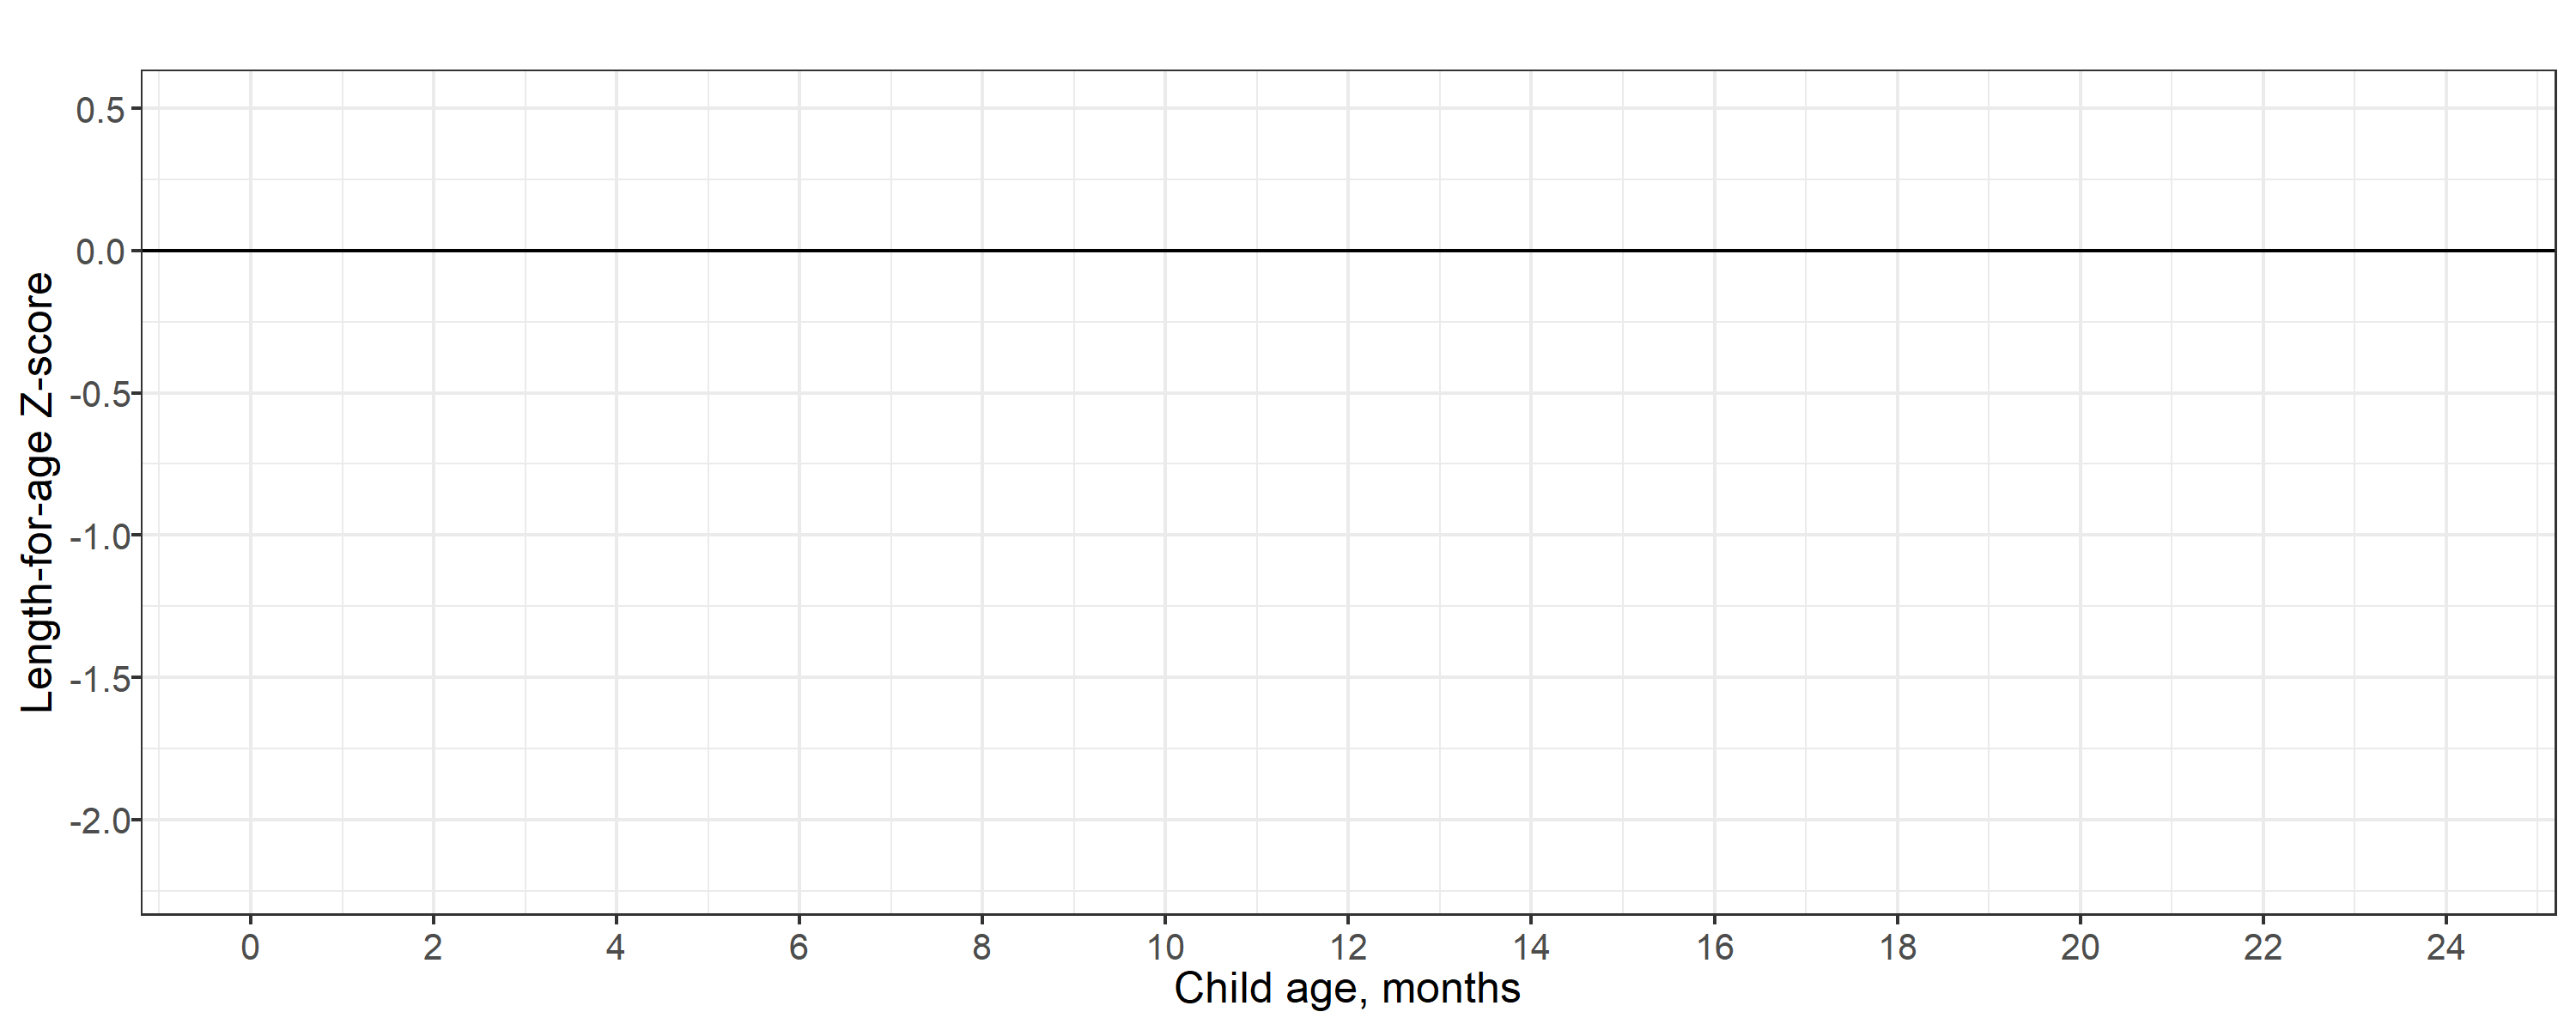
\includegraphics[width=41.67in]{C:/Users/andre/Documents/HBGDki/stunting/ki-longitudinal-manuscripts/figures/stunting/fig-laz-2-mean-overall_region--allage-primary}

\subsection{Cohorts that measured monthly from birth to 24
months}\label{cohorts-that-measured-monthly-from-birth-to-24-months}

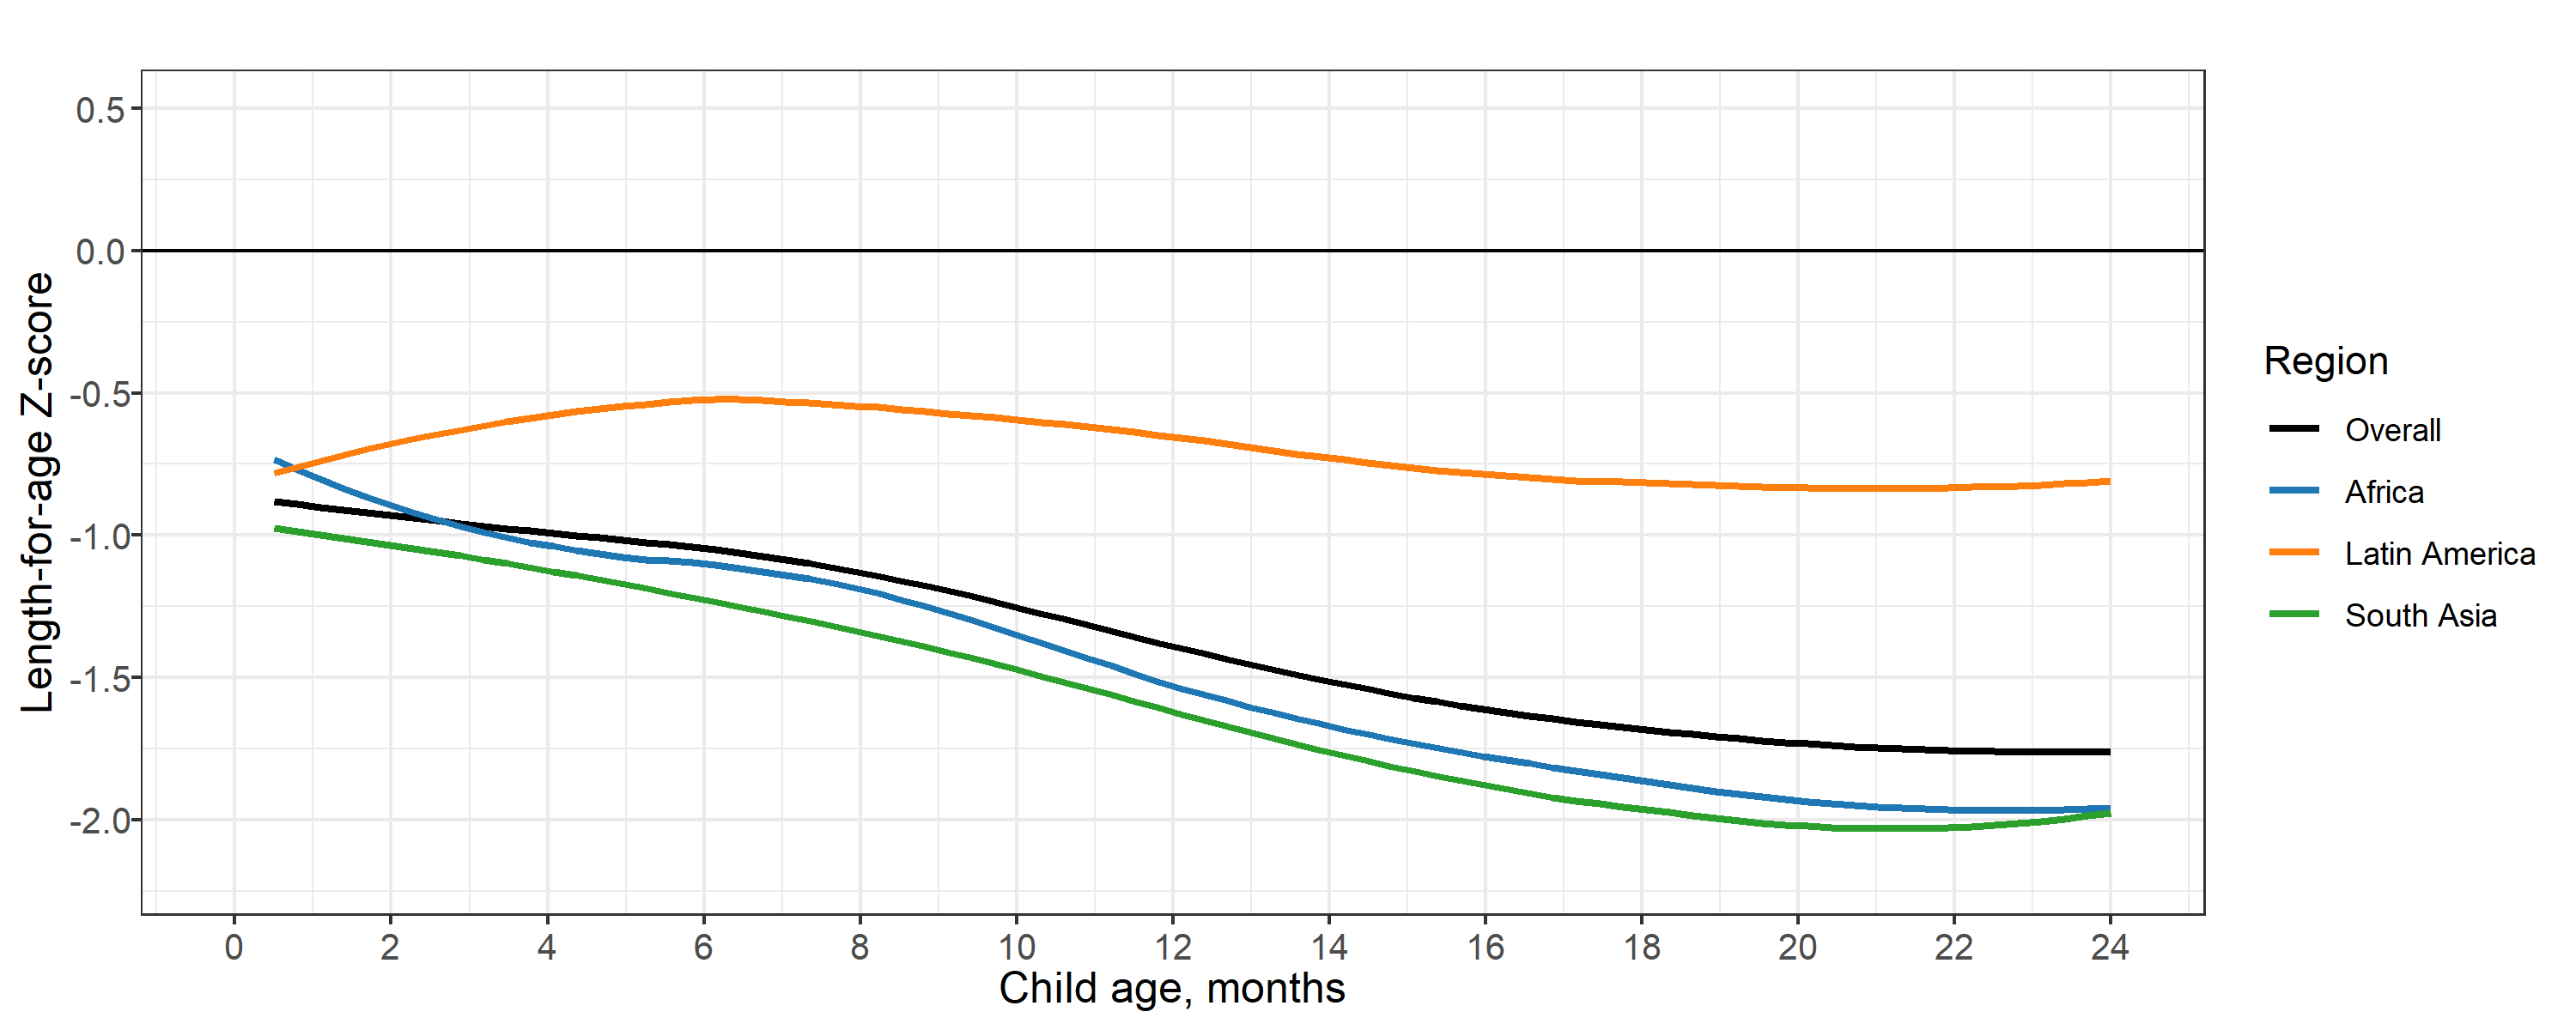
\includegraphics[width=41.67in]{C:/Users/andre/Documents/HBGDki/stunting/ki-longitudinal-manuscripts/figures/stunting/fig-laz-2-mean-overall_region--allage-month24}

\section{Age-specific severe stunting
prevalence}\label{age-specific-severe-stunting-prevalence-1}

\subsection{All eligible cohorts}\label{all-eligible-cohorts-1}

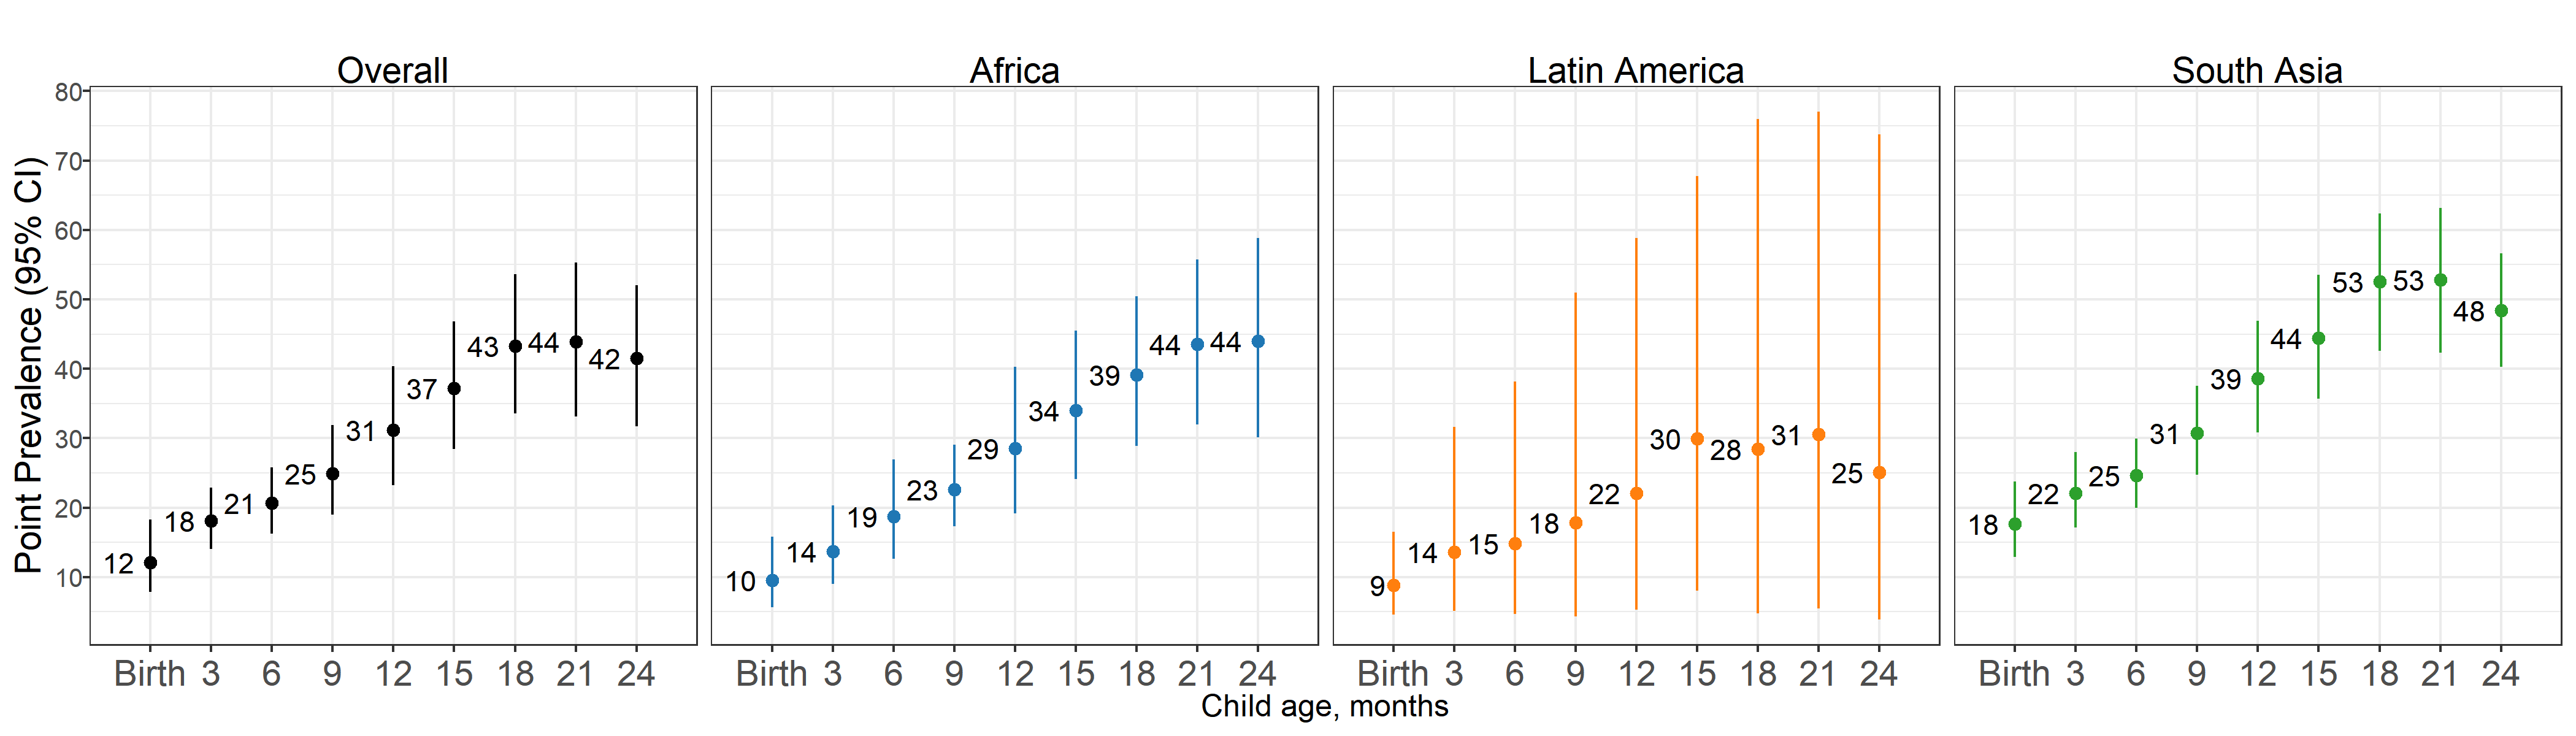
\includegraphics[width=58.33in]{C:/Users/andre/Documents/HBGDki/stunting/ki-longitudinal-manuscripts/figures/stunting/fig-stunt-2-prev-overall_region--allage-primary}

\subsection{Cohorts that measured monthly from birth to 24
months}\label{cohorts-that-measured-monthly-from-birth-to-24-months-1}

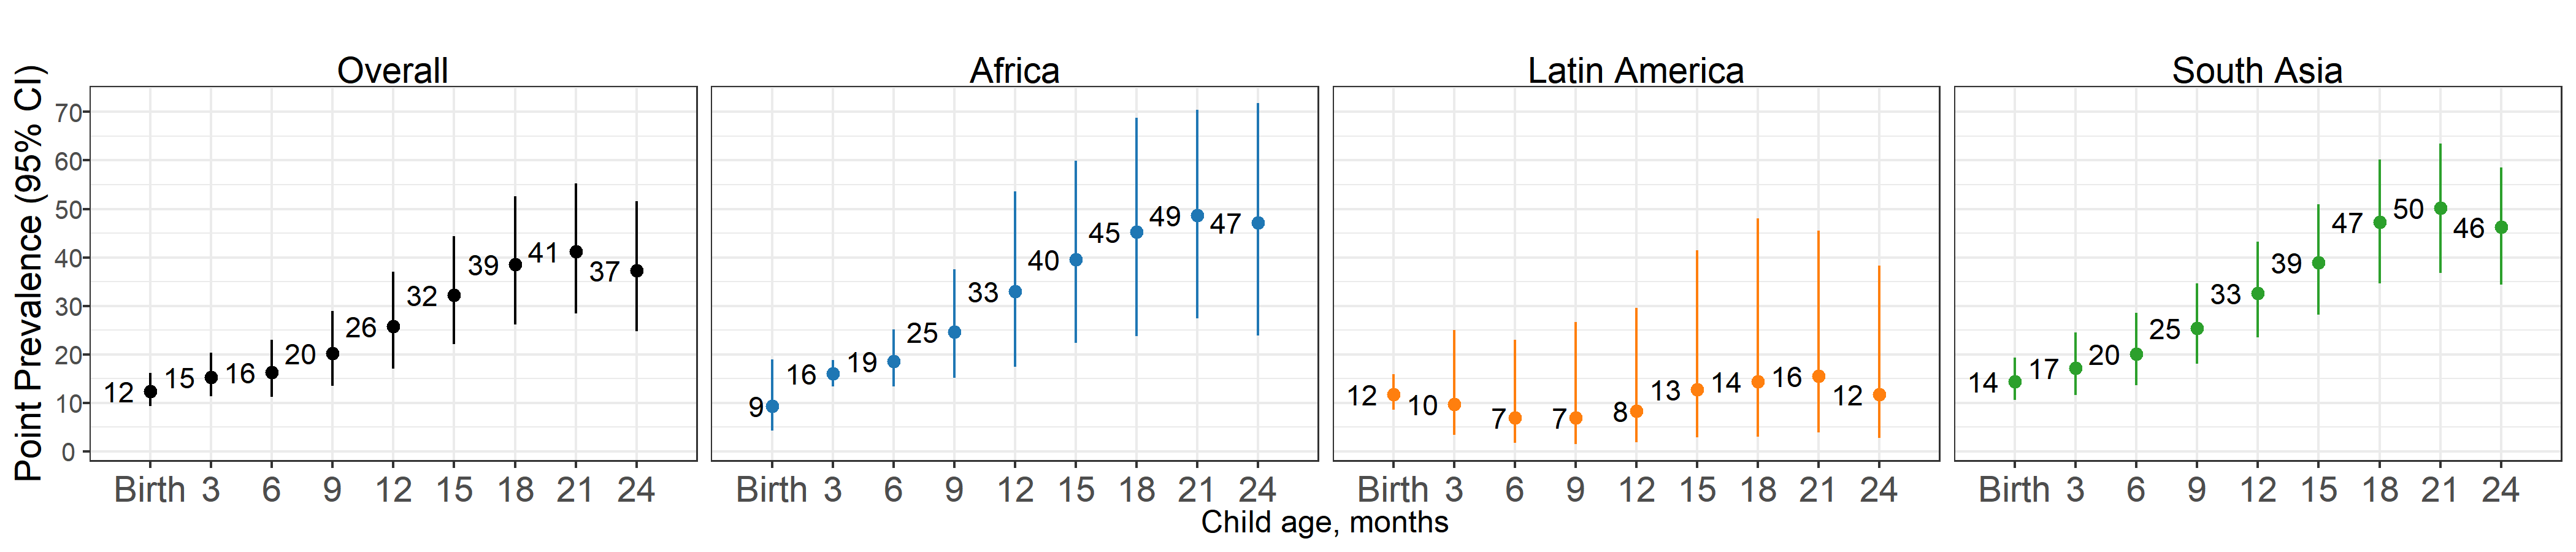
\includegraphics[width=58.33in]{C:/Users/andre/Documents/HBGDki/stunting/ki-longitudinal-manuscripts/figures/stunting/fig-stunt-2-prev-overall_region--allage-month24}

\section{Age-specific severe stunting
incidence}\label{age-specific-severe-stunting-incidence-1}

\subsection{All eligible cohorts}\label{all-eligible-cohorts-2}

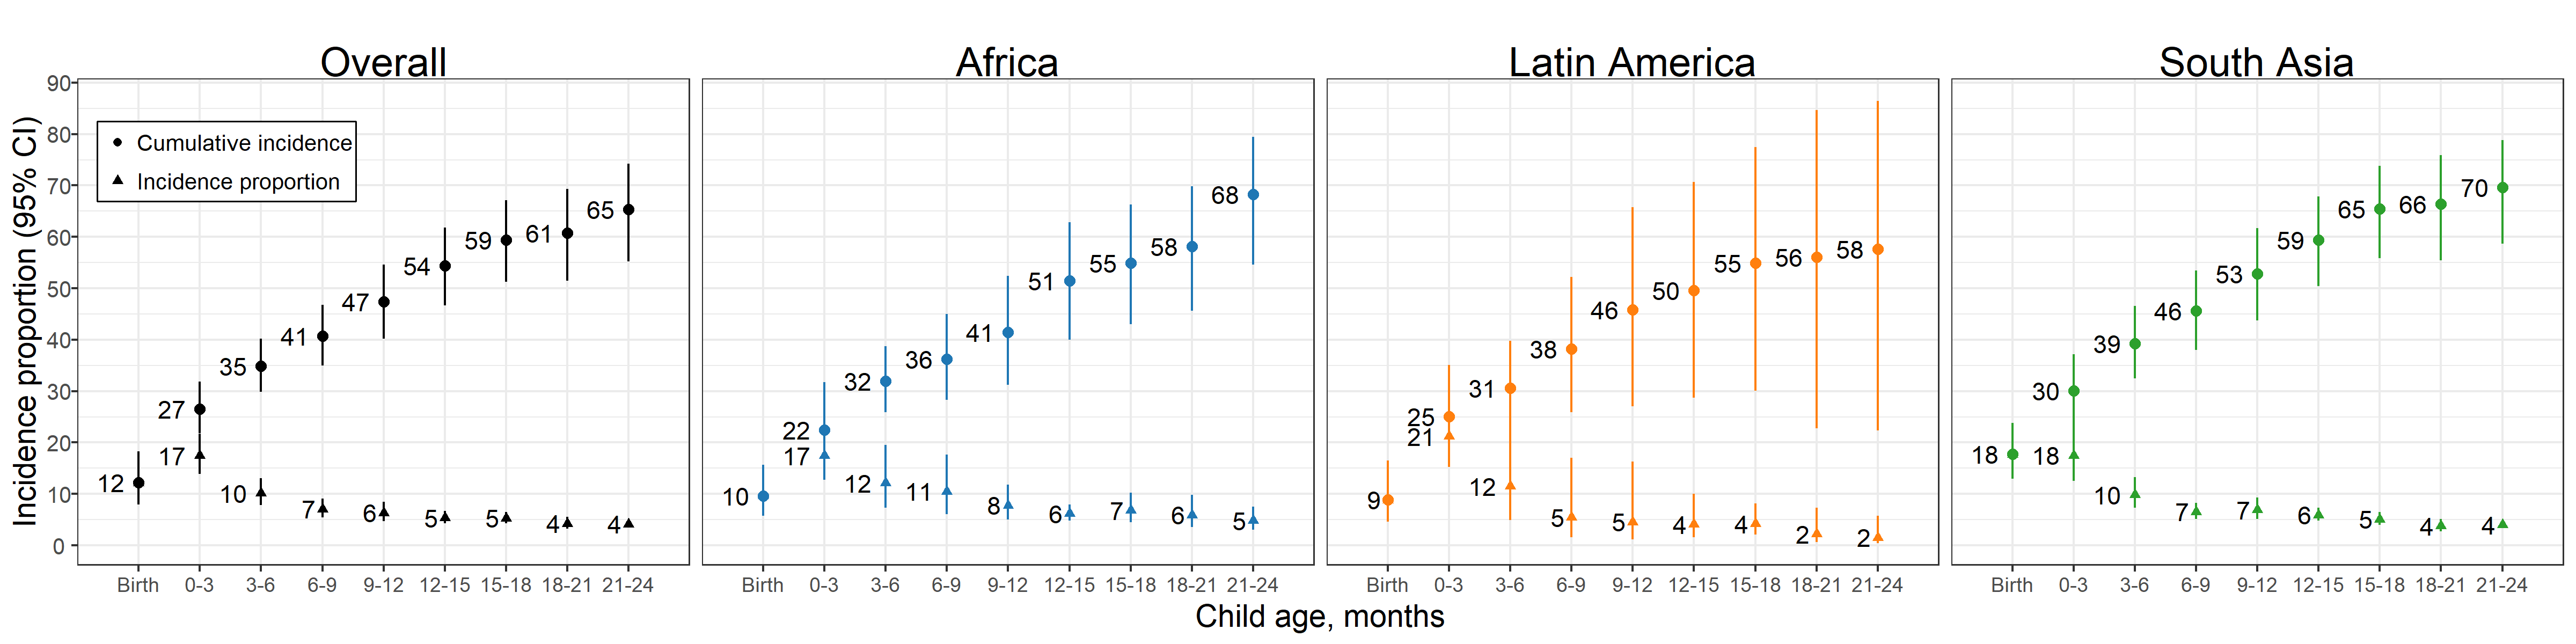
\includegraphics[width=66.67in]{C:/Users/andre/Documents/HBGDki/stunting/ki-longitudinal-manuscripts/figures/stunting/fig-stunt-2-inc-overall_region--allage-primary}

\subsection{Cohorts that measured monthly from birth to 24
months}\label{cohorts-that-measured-monthly-from-birth-to-24-months-2}

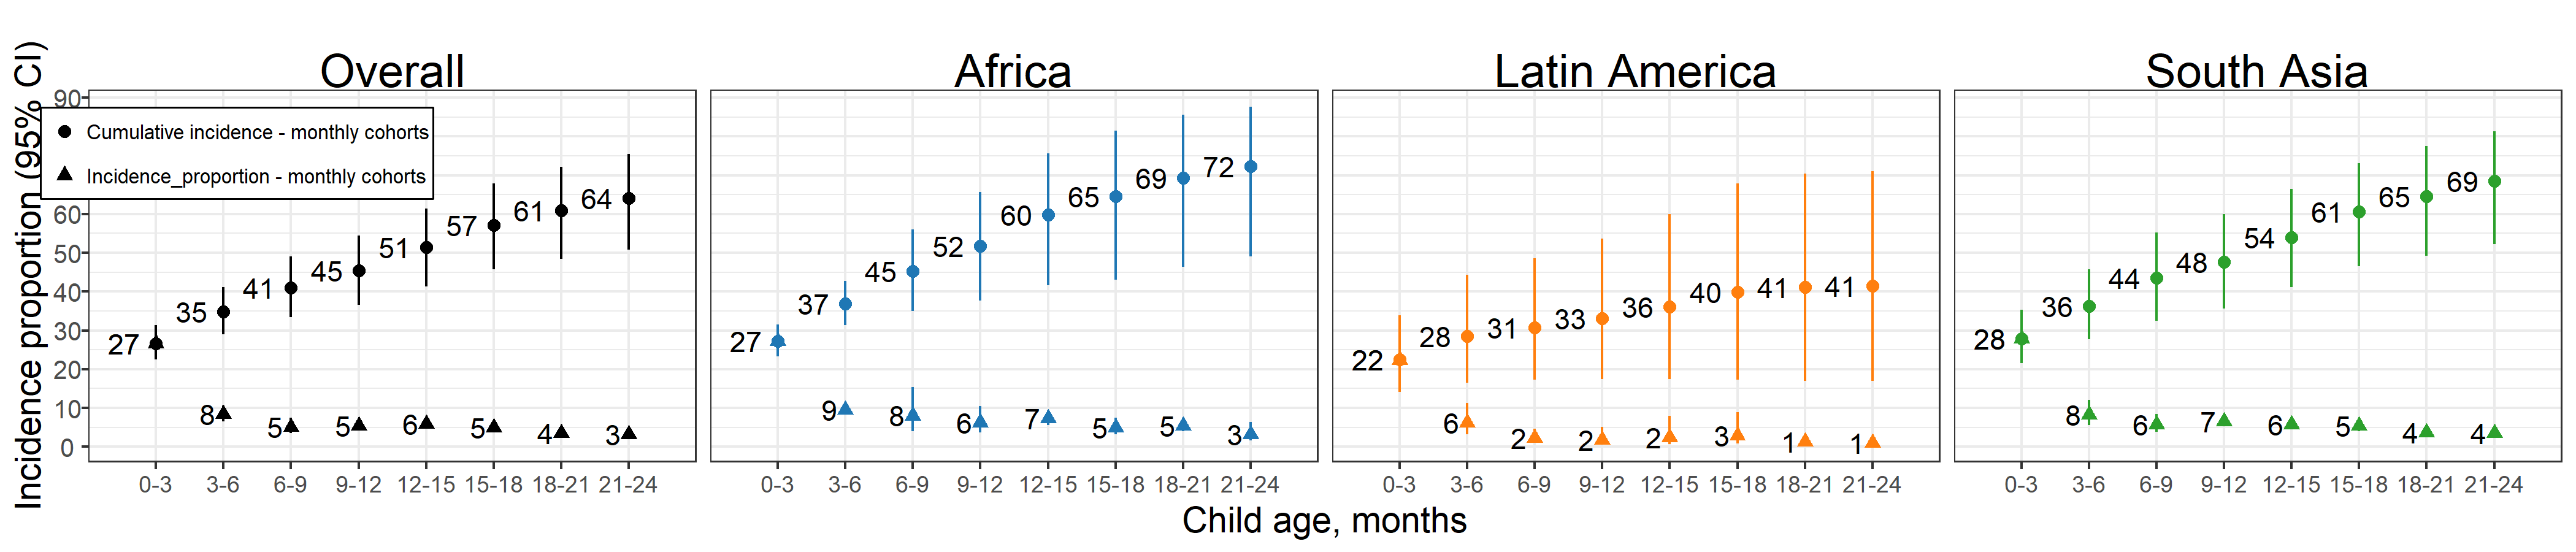
\includegraphics[width=58.33in]{C:/Users/andre/Documents/HBGDki/stunting/ki-longitudinal-manuscripts/figures/stunting/fig-stunt-2-inc-overall_region--allage-month24}

\section{Linear growth velocity}\label{linear-growth-velocity}

\subsection{All eligible cohorts}\label{all-eligible-cohorts-3}

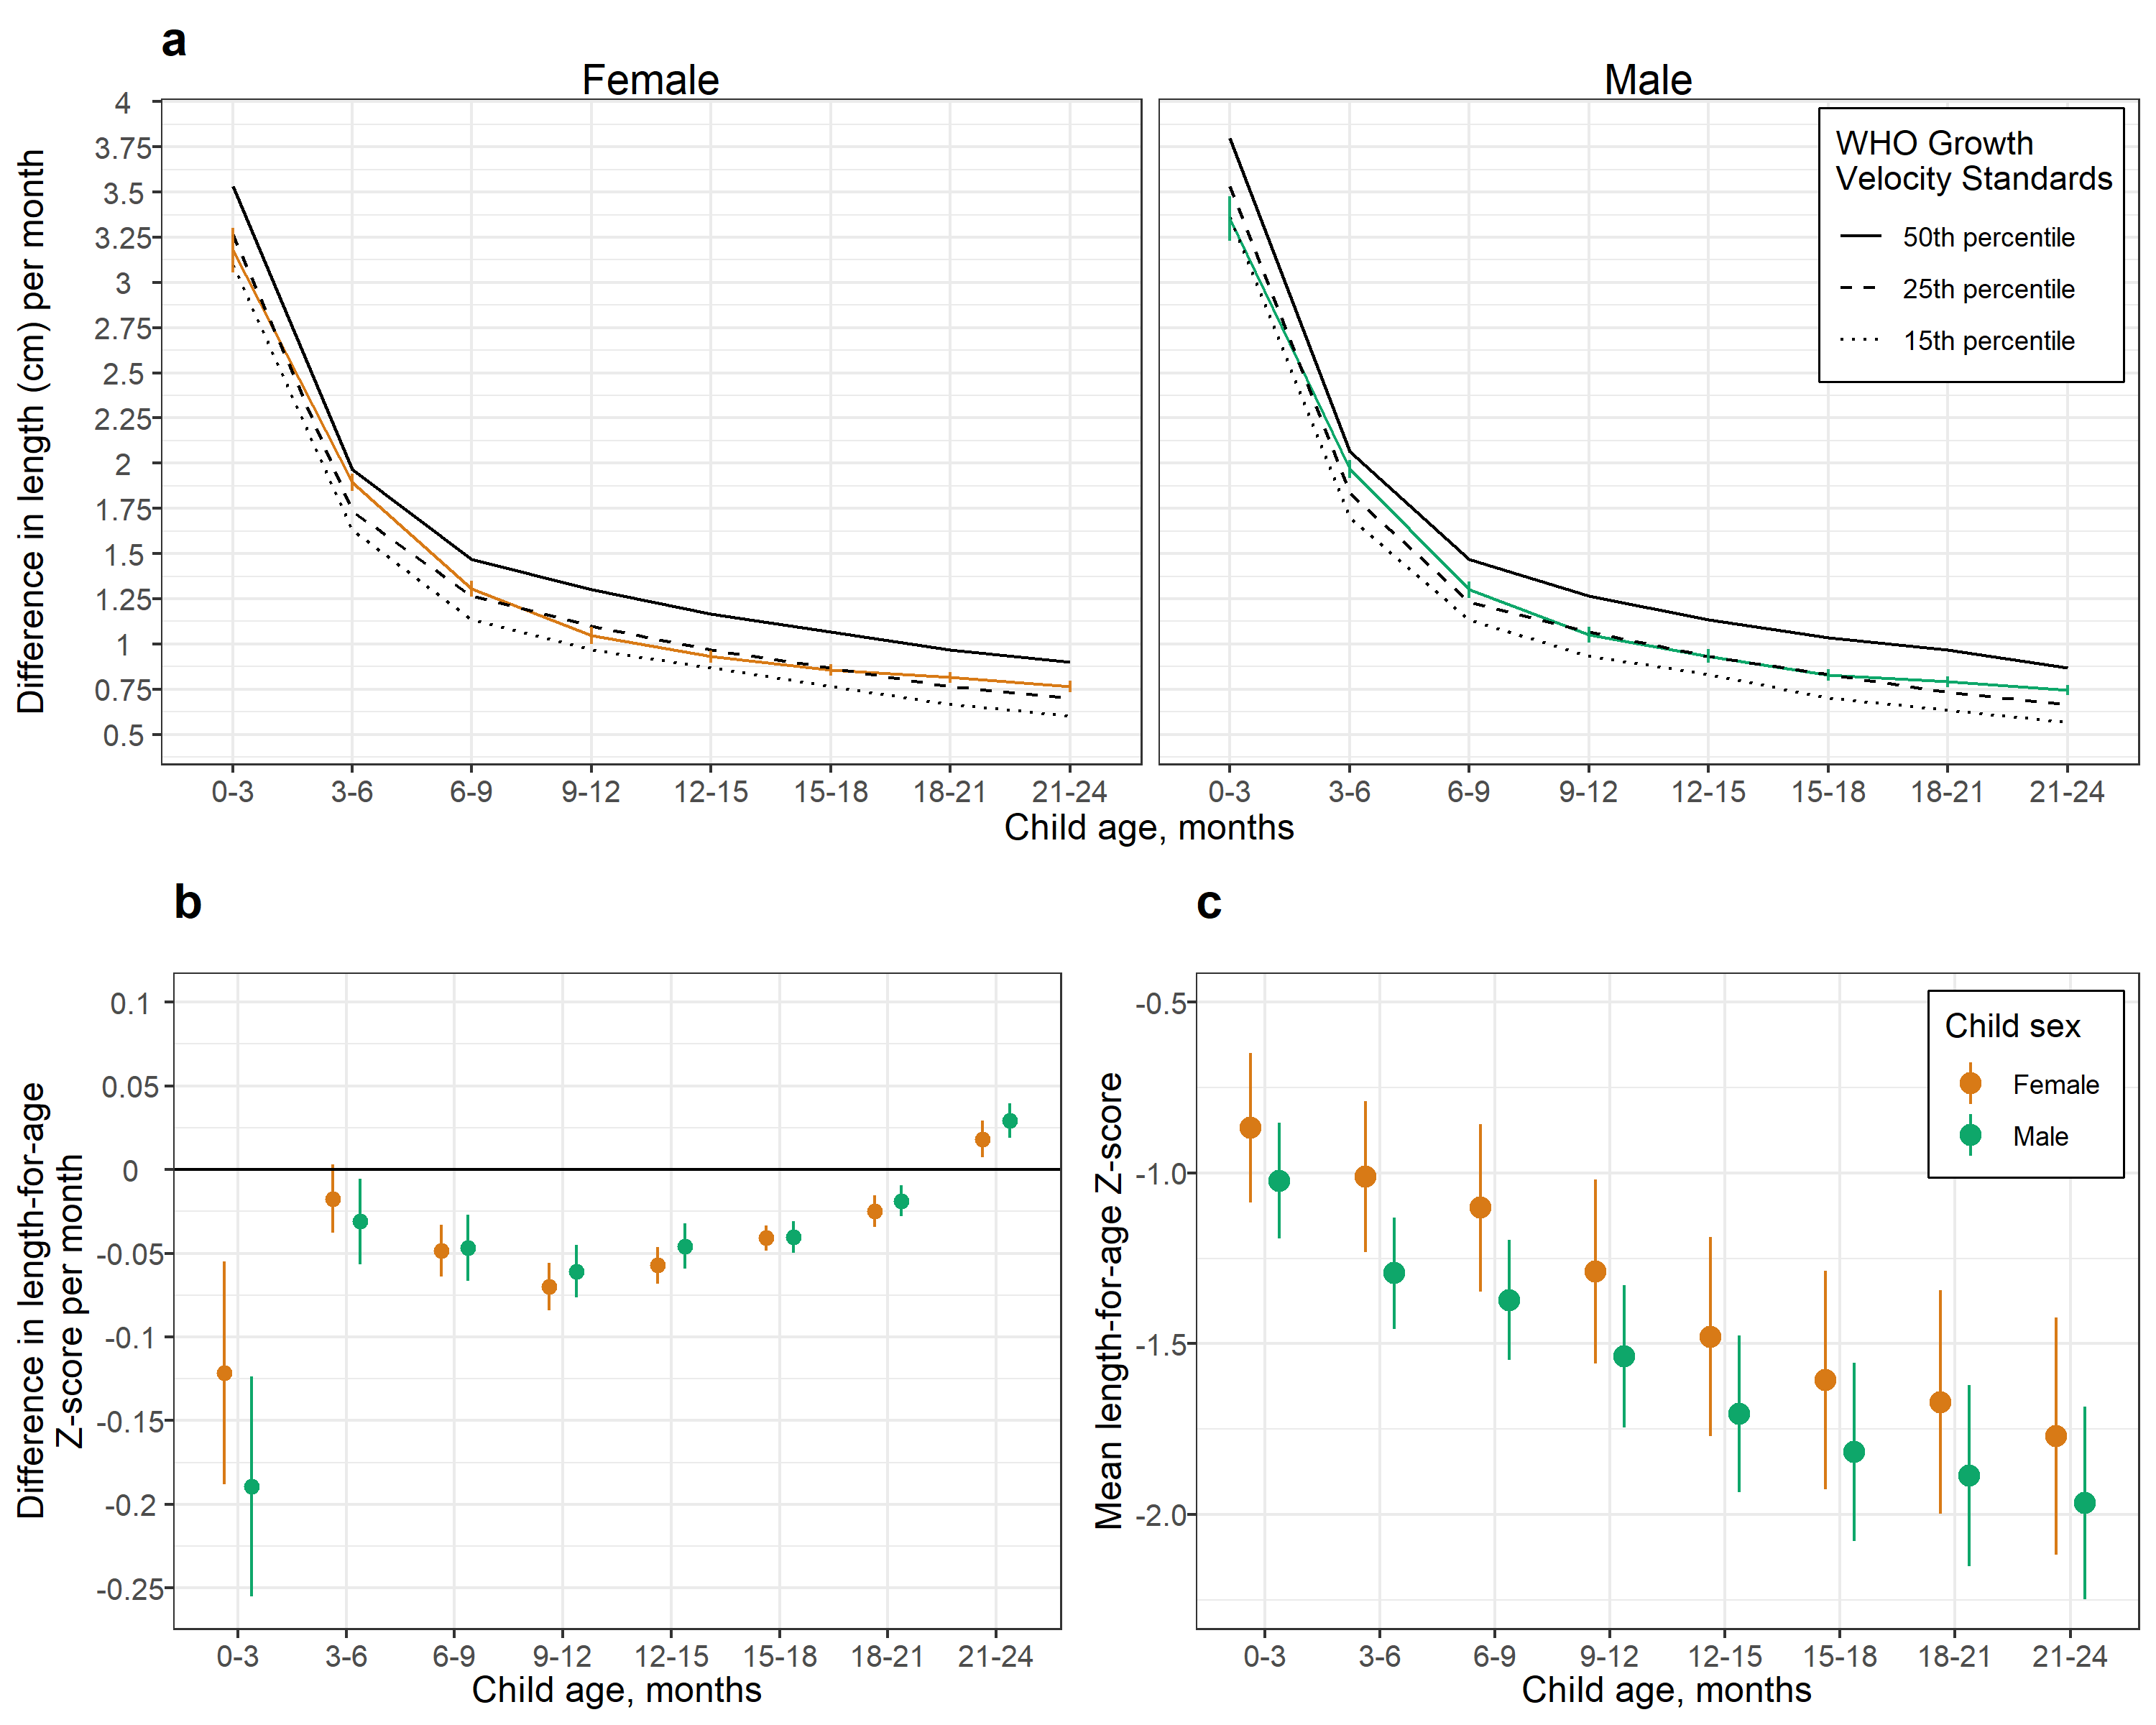
\includegraphics[width=41.67in]{C:/Users/andre/Documents/HBGDki/stunting/ki-longitudinal-manuscripts/figures/stunting/fig-stunt-2-vel-overall--allage-primary}
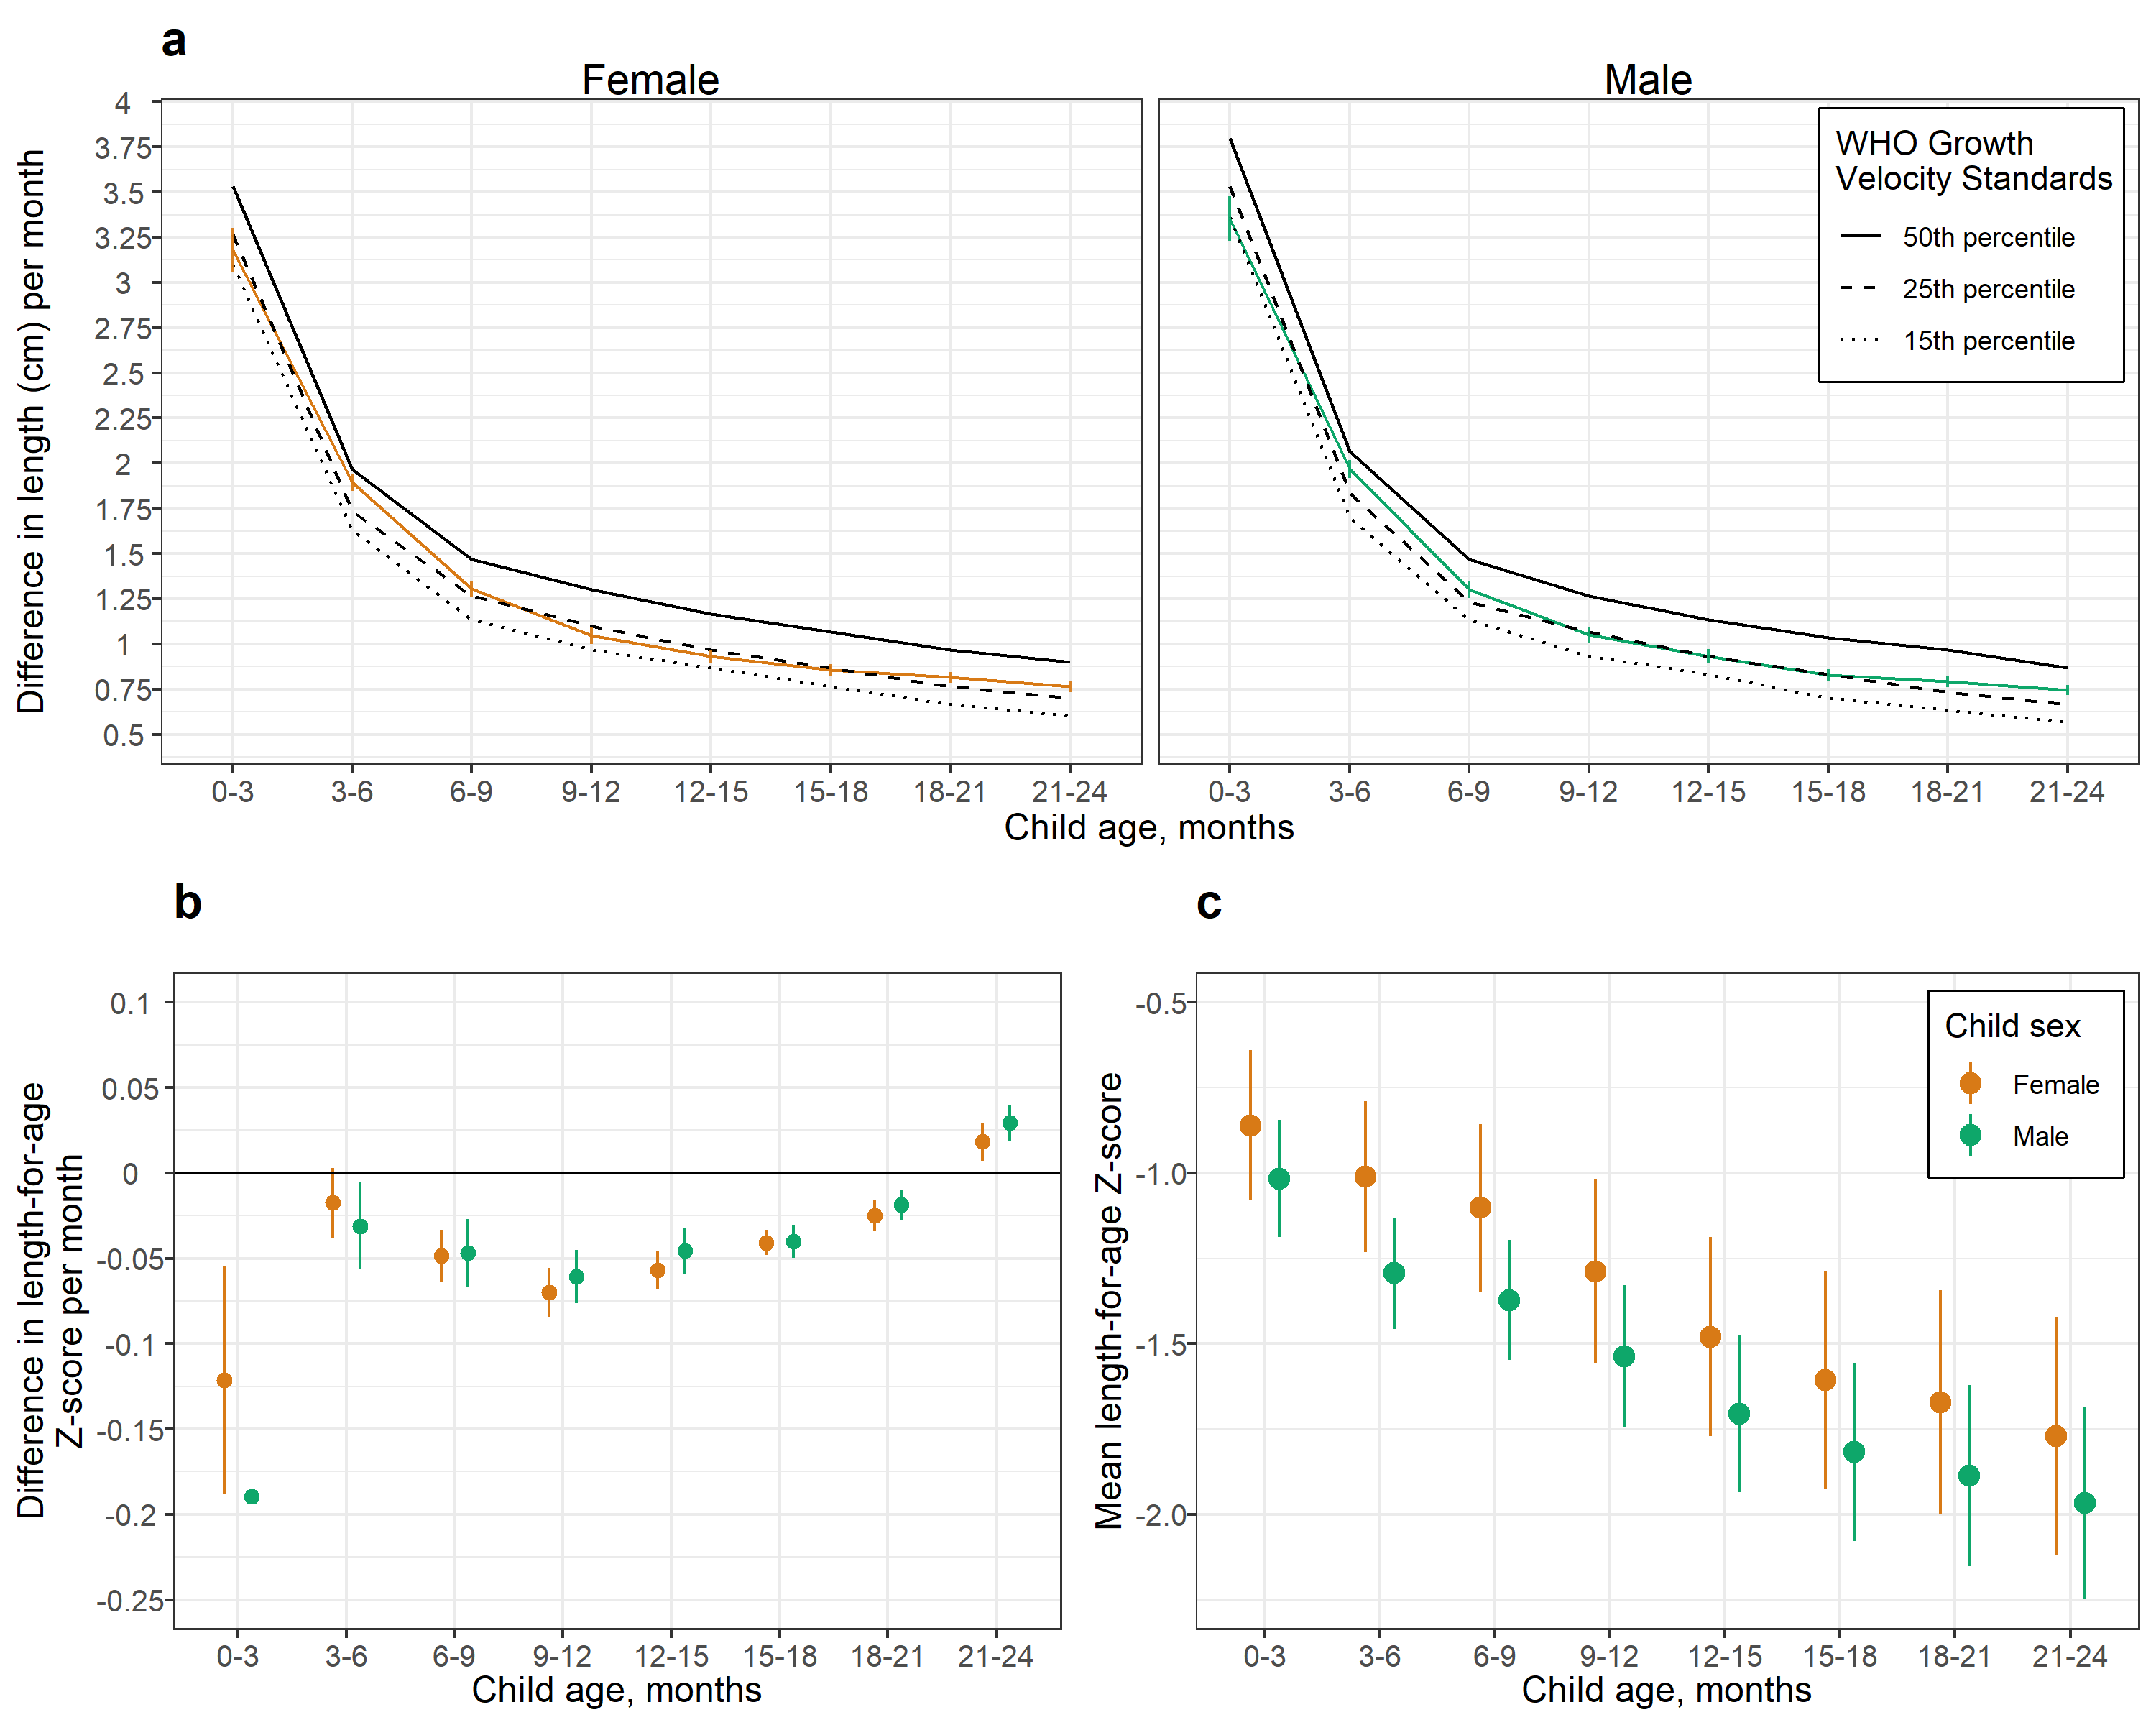
\includegraphics[width=41.67in]{figure-copies/fig-stunt-2-vel-overall--allage-primary}

\subsection{Cohorts that measured monthly from birth to 24
months}\label{cohorts-that-measured-monthly-from-birth-to-24-months-3}

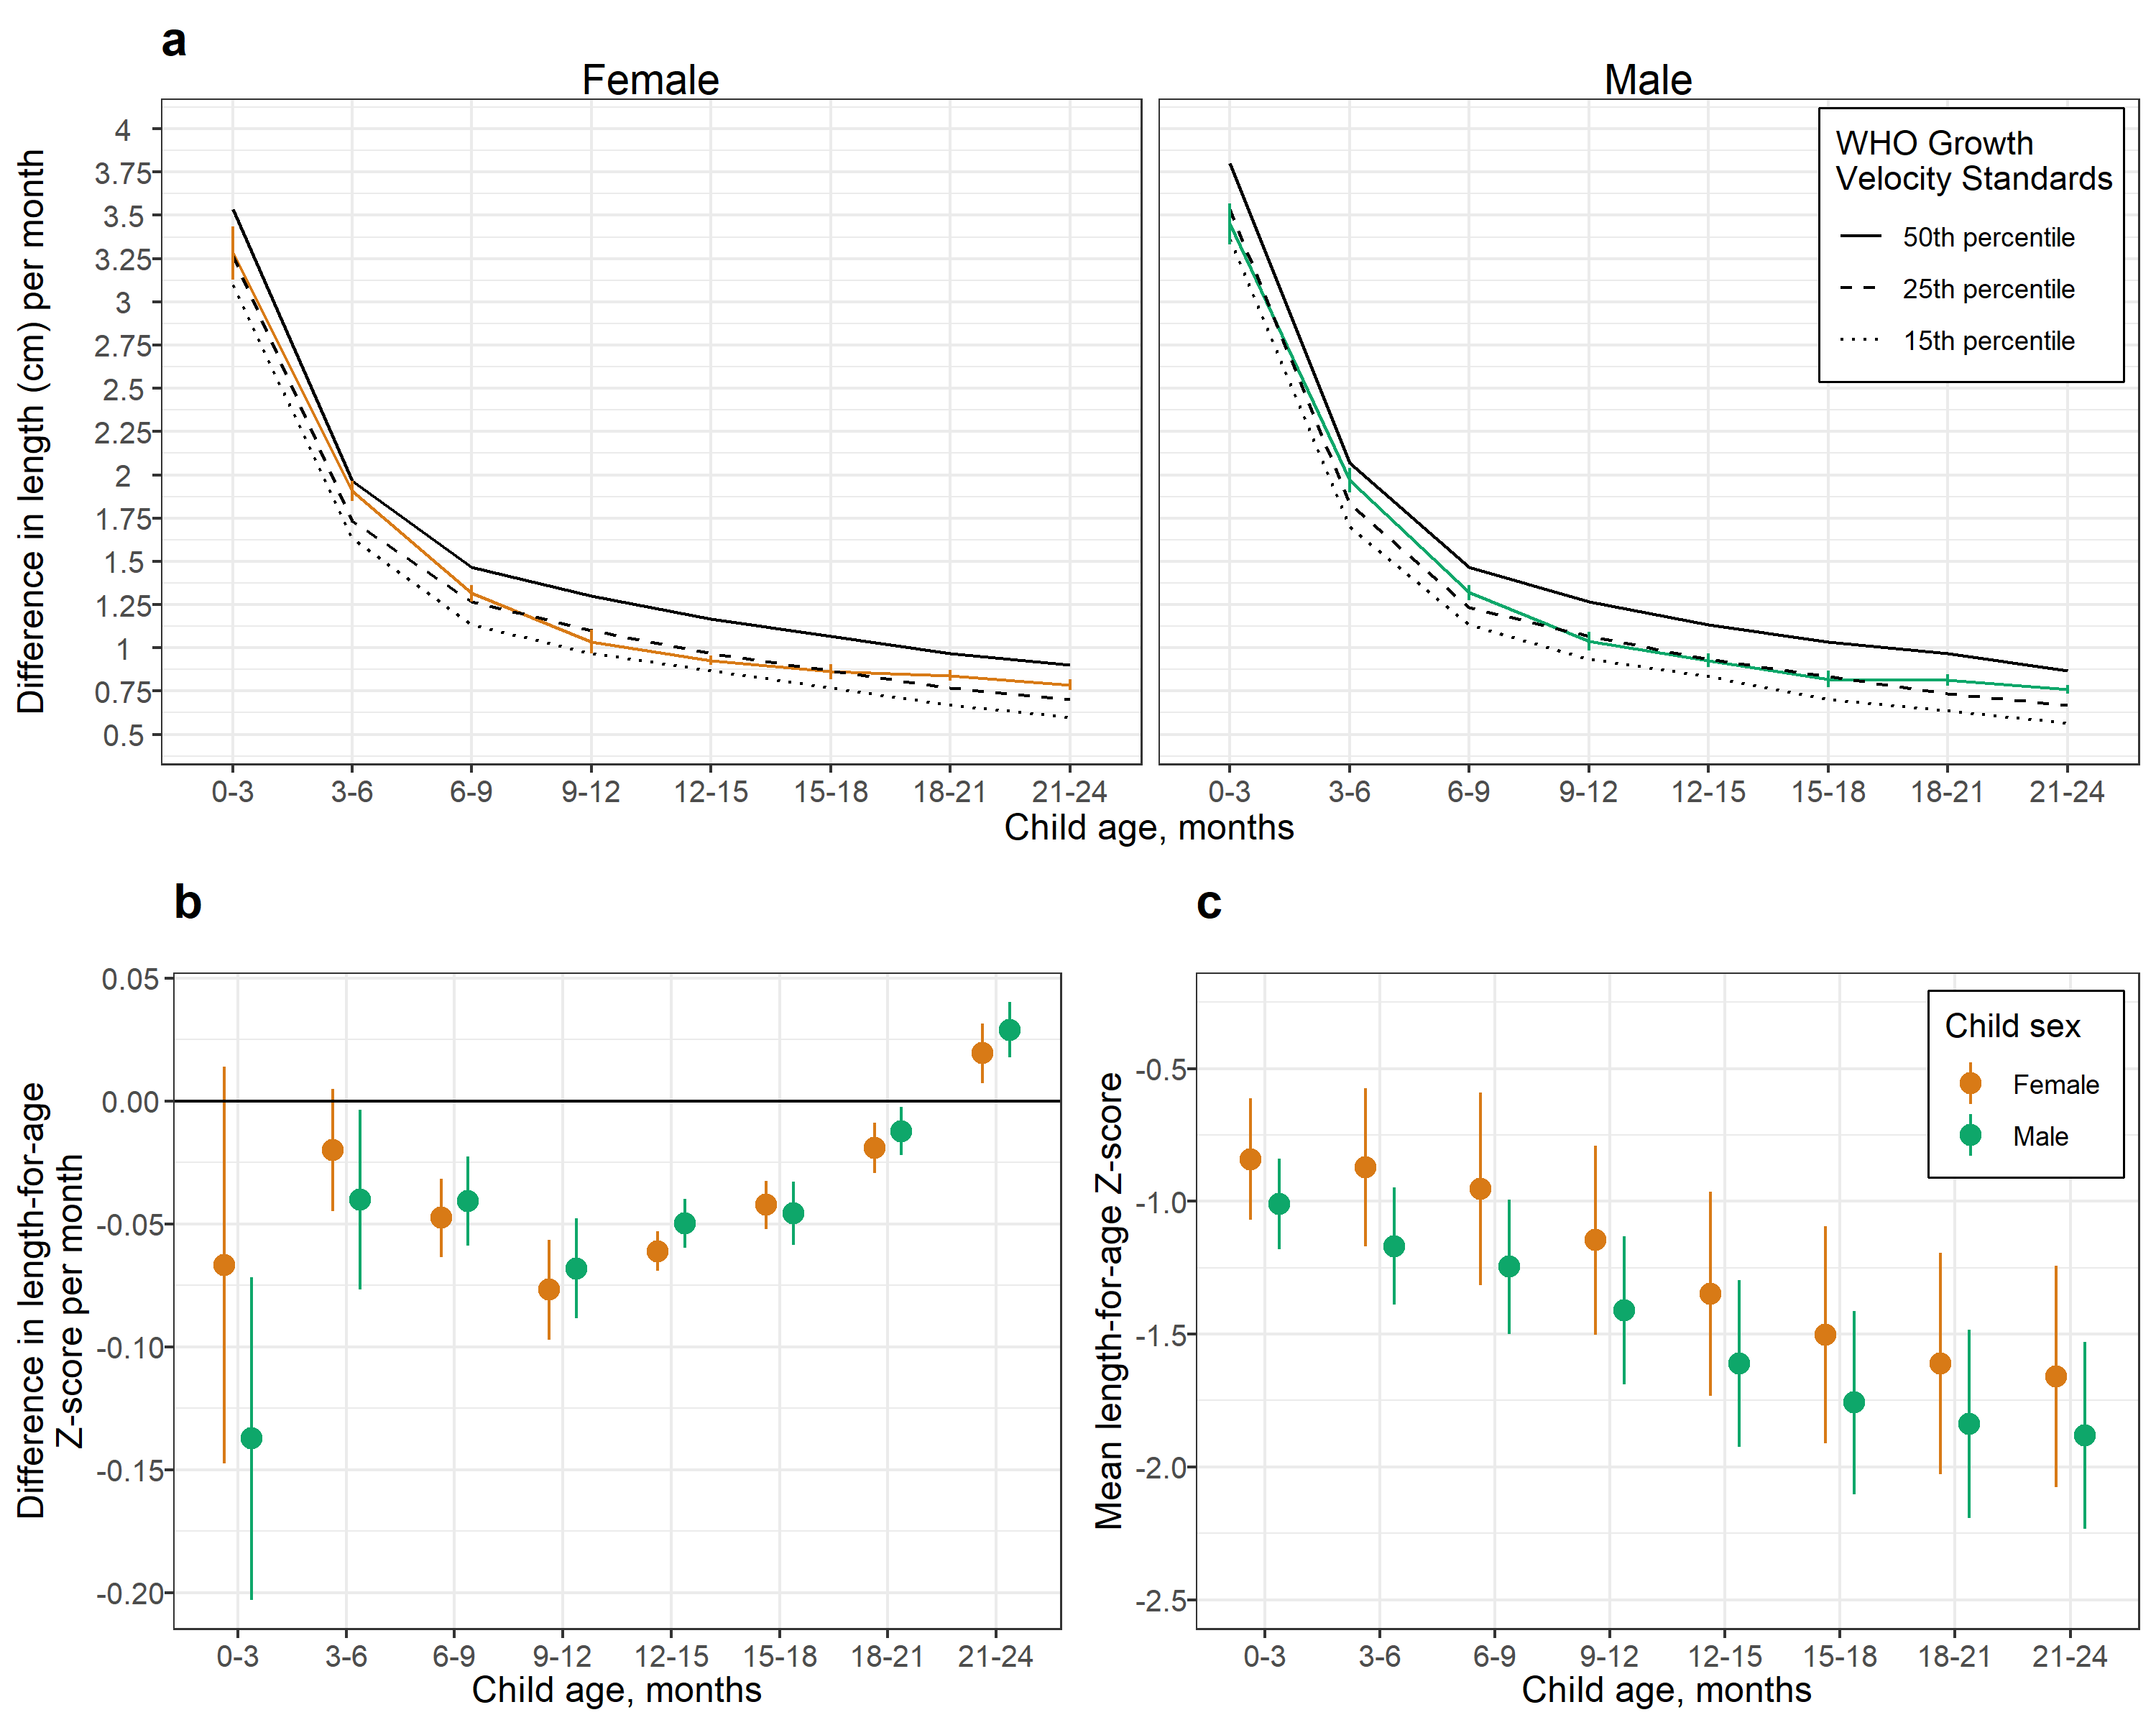
\includegraphics[width=41.67in]{C:/Users/andre/Documents/HBGDki/stunting/ki-longitudinal-manuscripts/figures/stunting/fig-stunt-2-vel-overall--allage-month24}

\chapter{Sensitivity analysis using fixed effects}\label{fixed-effects}

The primary analyses presented in this manuscript pooled across
individual studies using random effects. Inferences about estimates from
fixed effects models are restricted to only the included
studies.\footnote{Hedges, L. V. \& Vevea, J. L. Fixed- and
  random-effects models in meta-analysis. Psychol. Methods 3, 486--504
  (1998).} The random effects approach was more conservative in the
presence of study heterogeneity, as evidenced by larger confidence
intervals around each point estimates. Overall, the inference from
results produced by each method was similar.

\section{Age-specific prevalence}\label{age-specific-prevalence-2}

\subsection{Random effects}\label{random-effects}

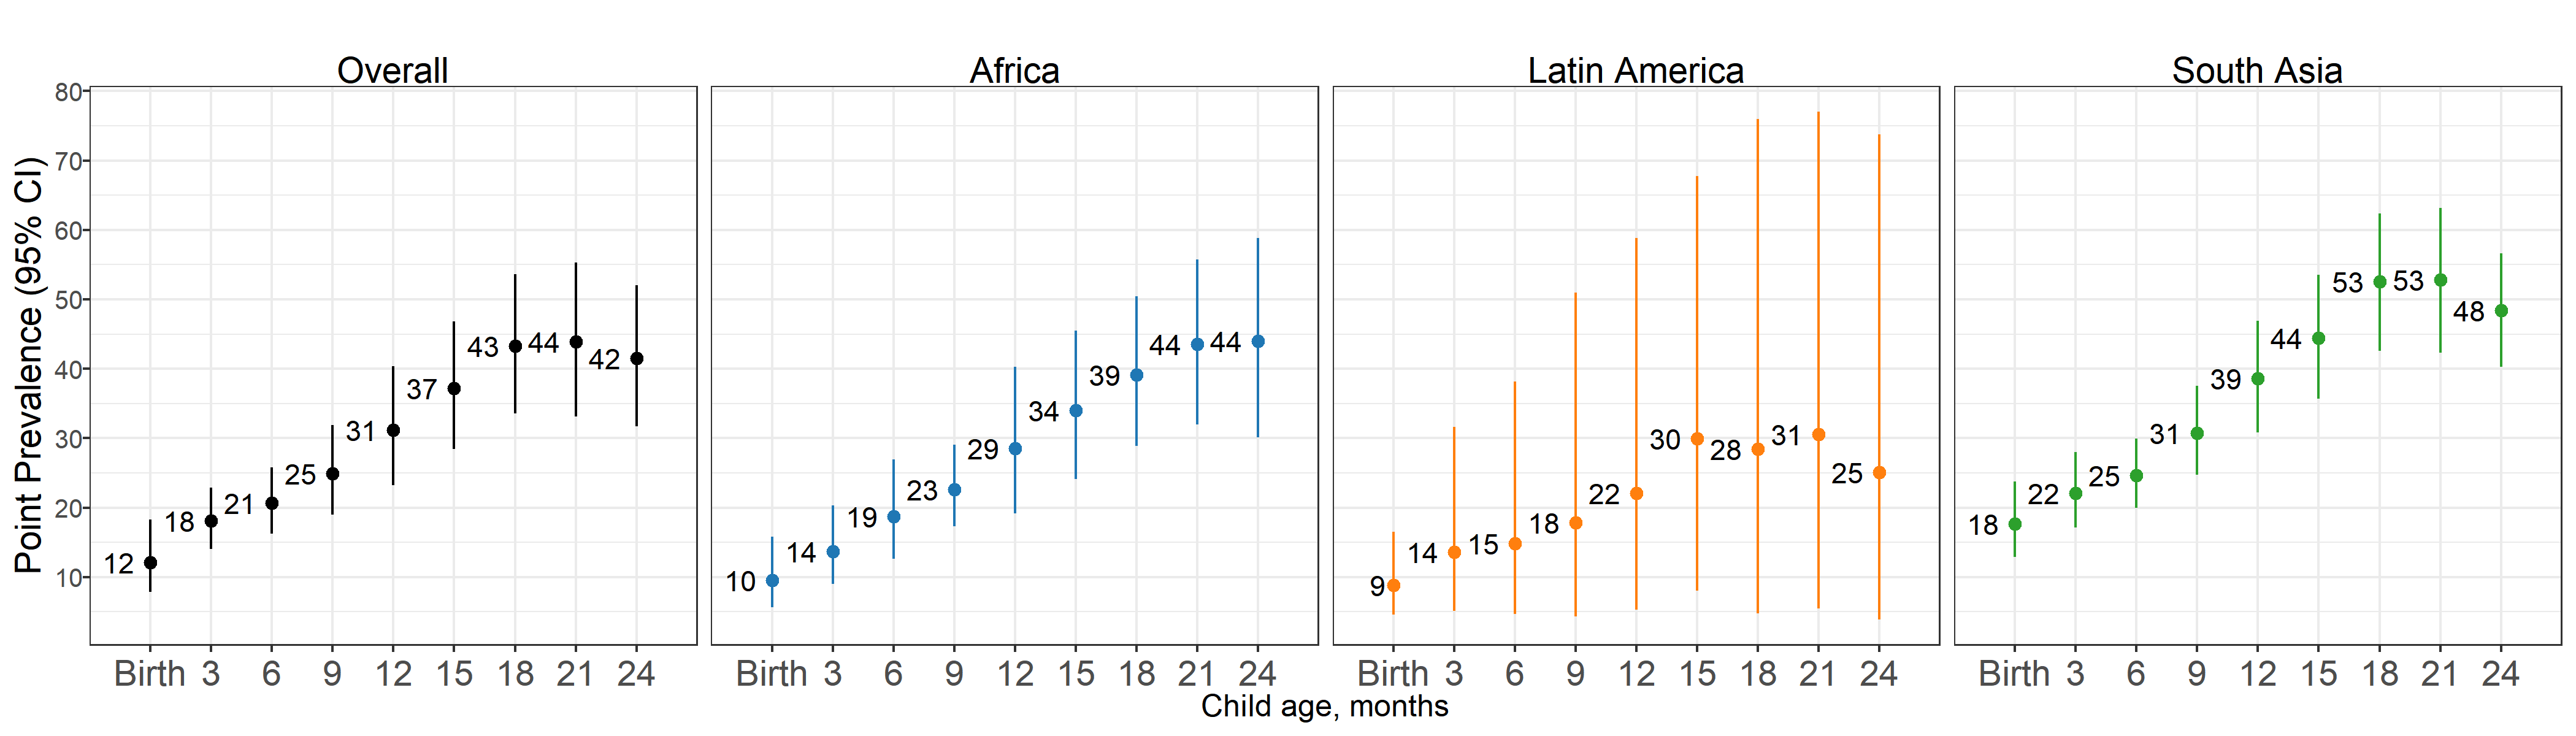
\includegraphics[width=58.33in]{C:/Users/andre/Documents/HBGDki/stunting/ki-longitudinal-manuscripts/figures/stunting/fig-stunt-2-prev-overall_region--allage-primary}

\subsection{Fixed effects}\label{fixed-effects}

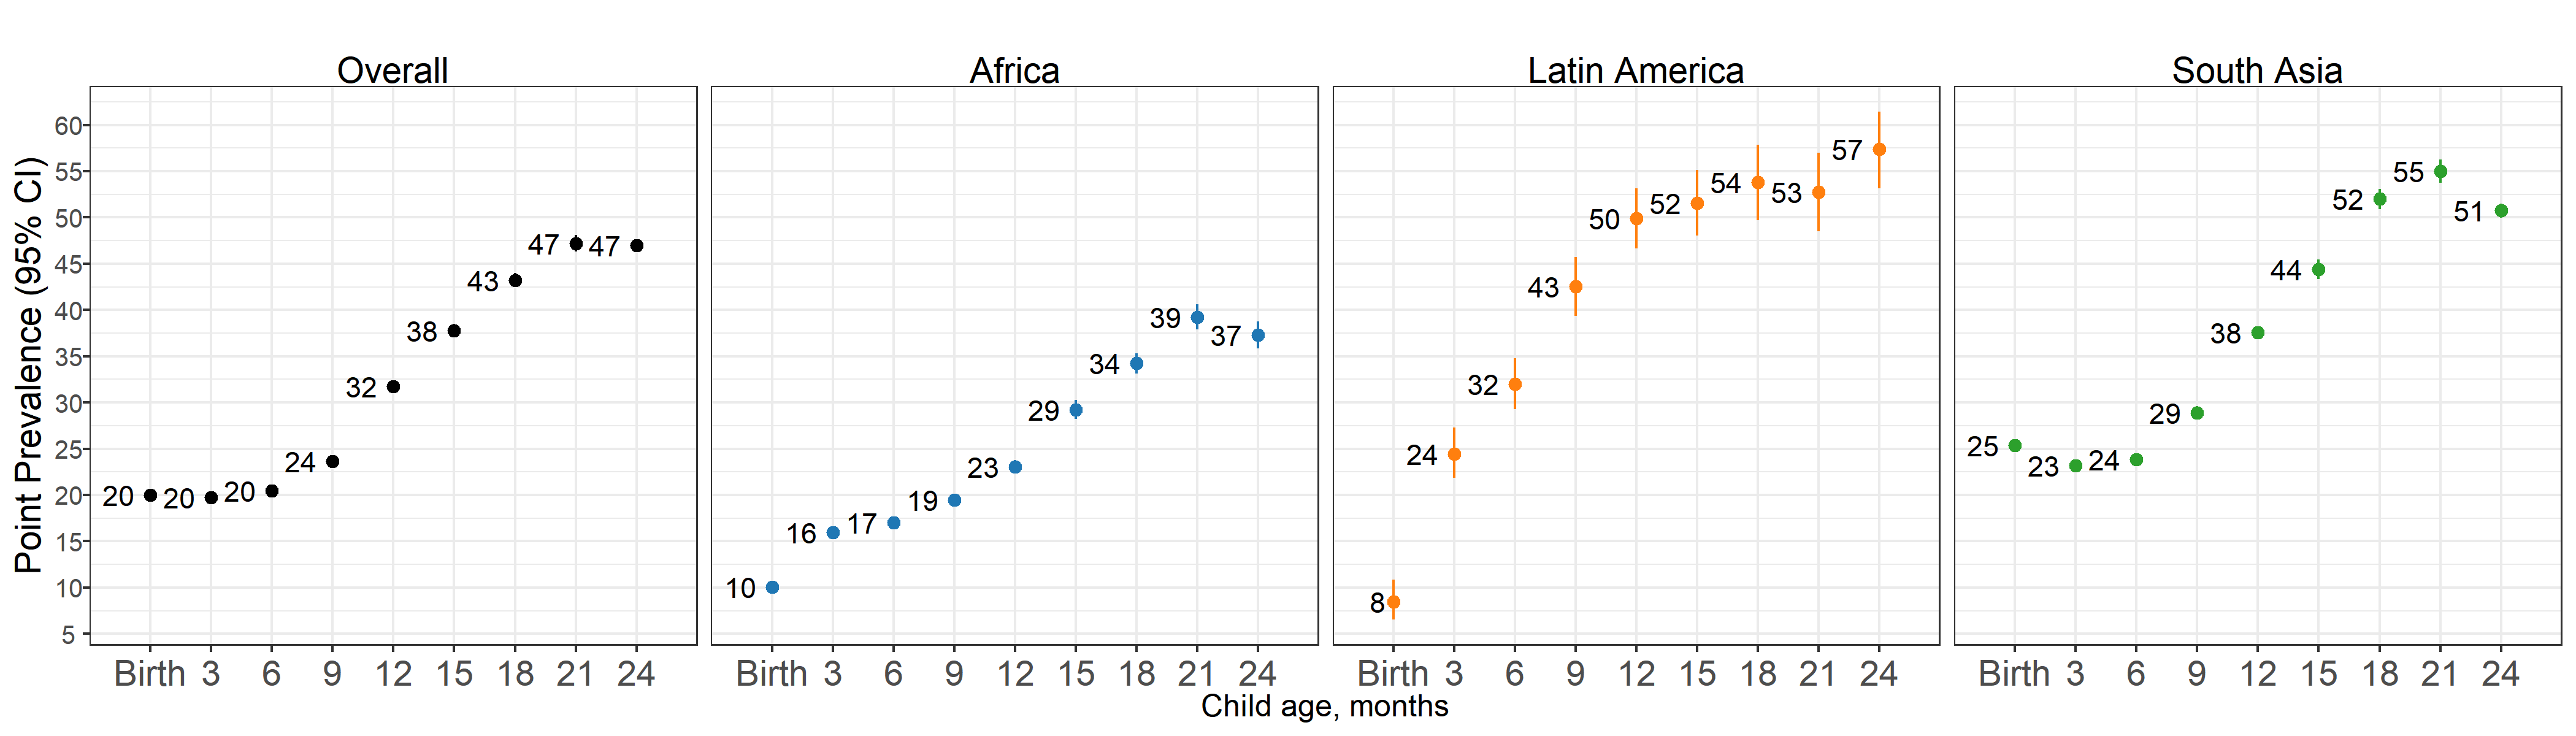
\includegraphics[width=58.33in]{C:/Users/andre/Documents/HBGDki/stunting/ki-longitudinal-manuscripts/figures/stunting/fig-stunt-2-prev-overall_region--allage-fe}

{[}ADD CAPTION{]}

\section{Age-specific incidence}\label{age-specific-incidence-2}

\subsection{Random effects}\label{random-effects-1}

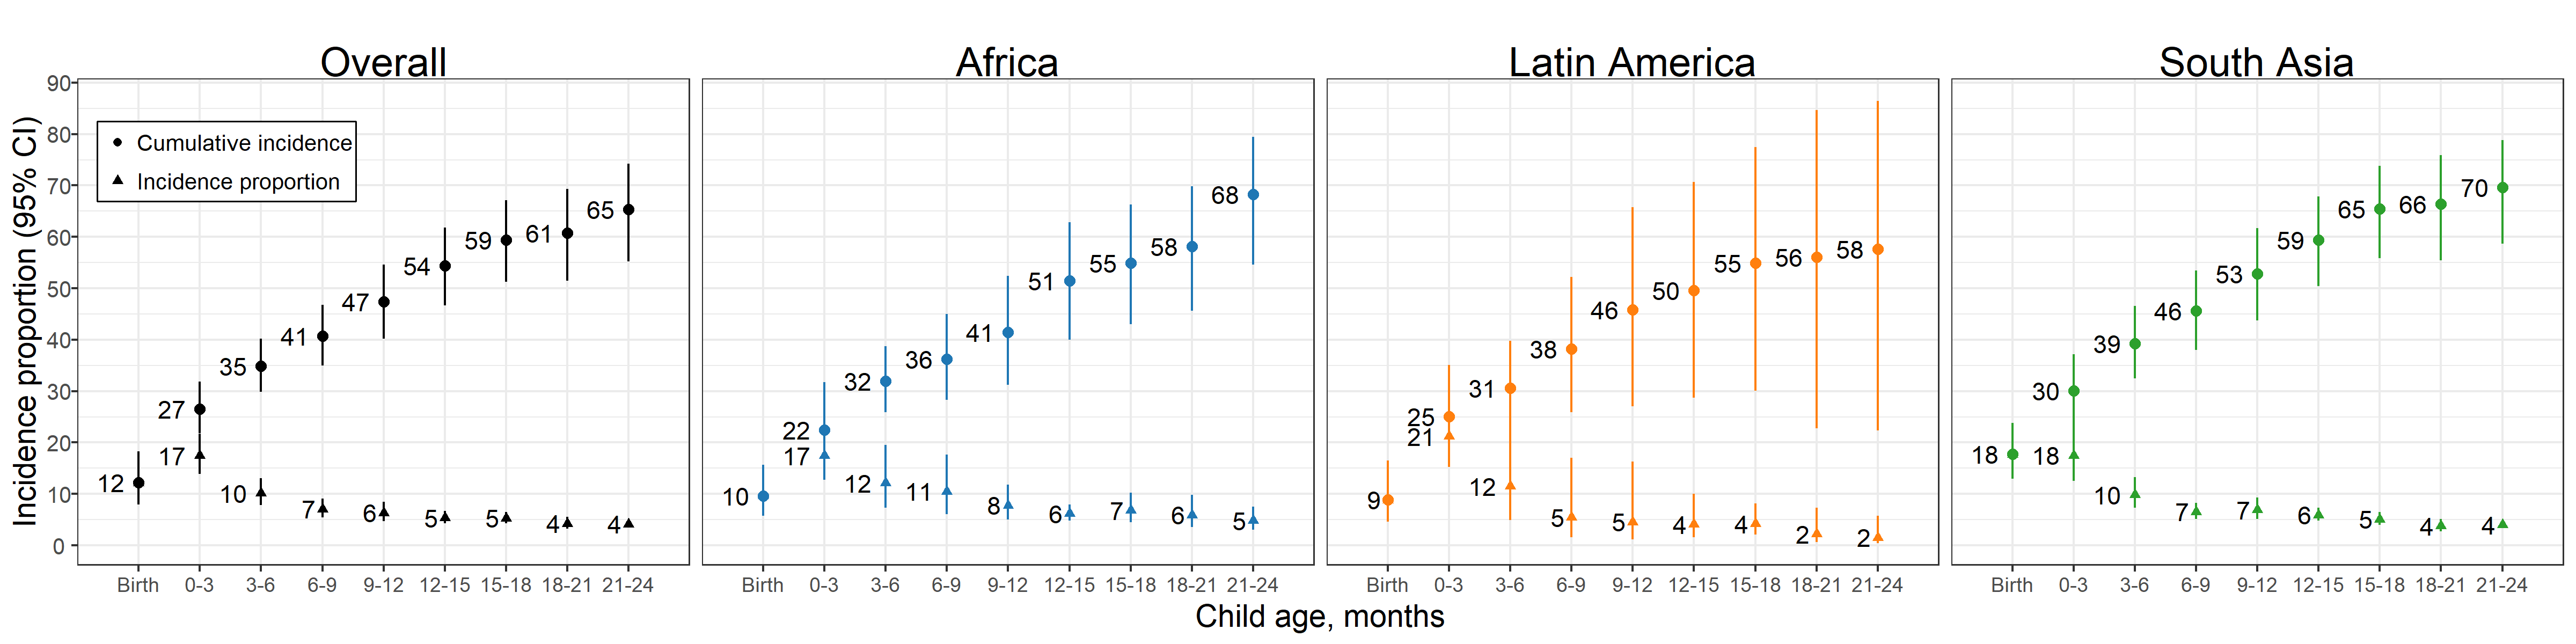
\includegraphics[width=66.67in]{C:/Users/andre/Documents/HBGDki/stunting/ki-longitudinal-manuscripts/figures/stunting/fig-stunt-2-inc-overall_region--allage-primary}

\subsection{Fixed effects}\label{fixed-effects-1}

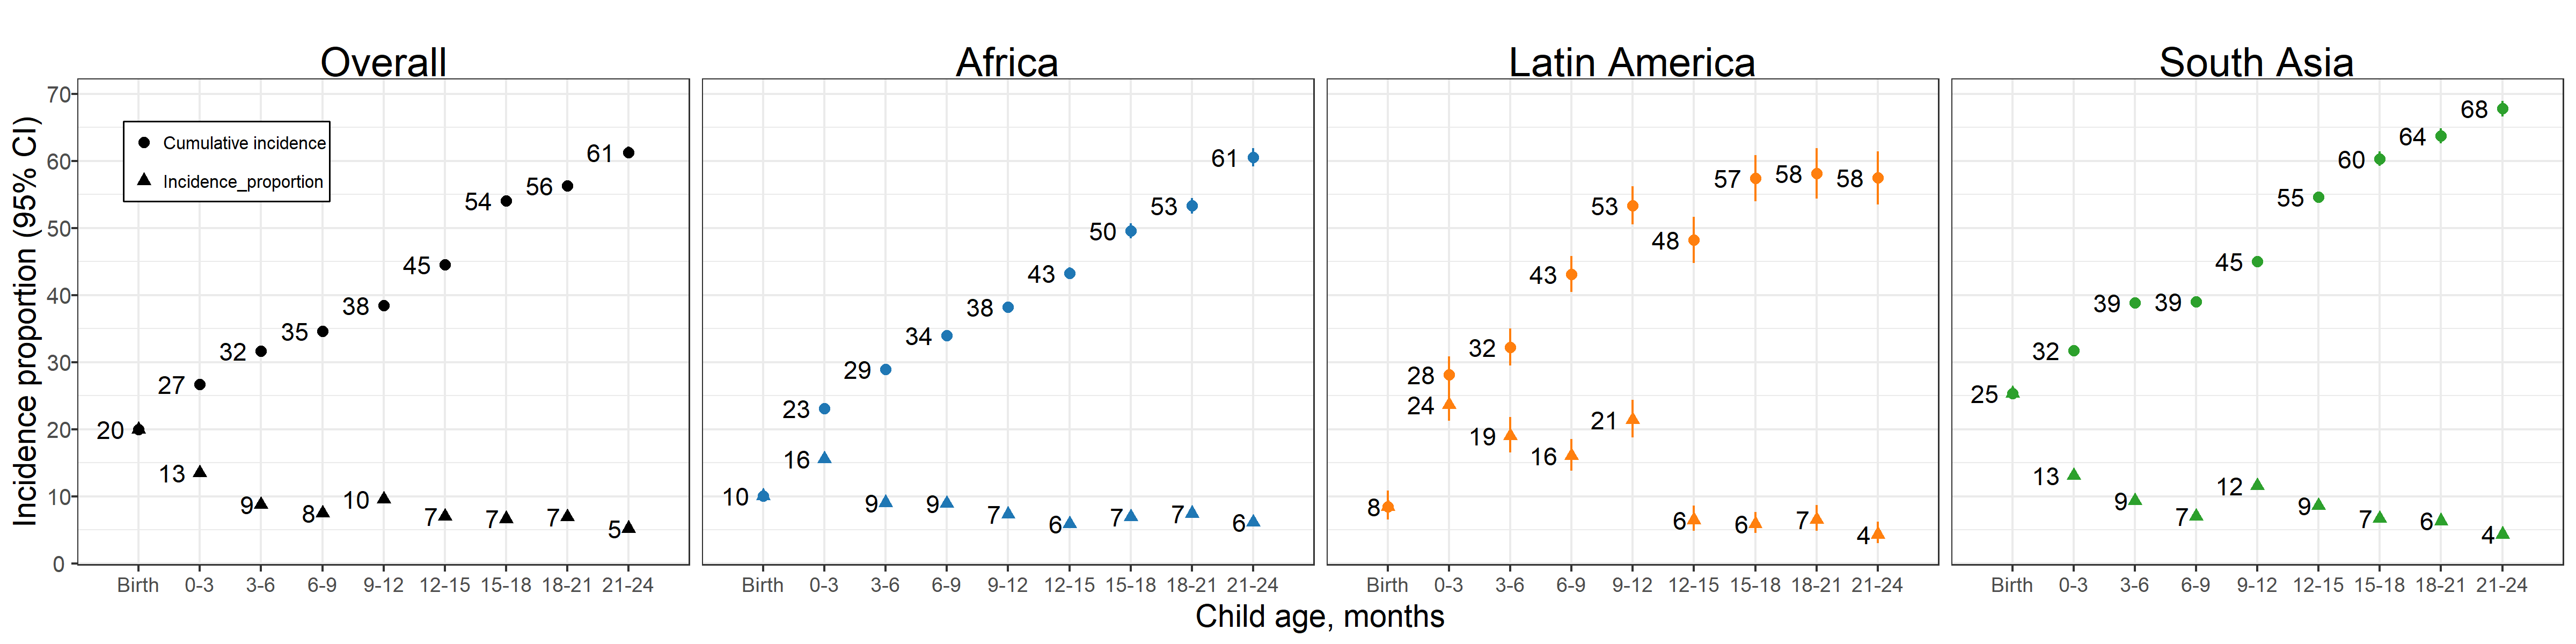
\includegraphics[width=66.67in]{C:/Users/andre/Documents/HBGDki/stunting/ki-longitudinal-manuscripts/figures/stunting/fig-stunt-2-inc-overall_region--allage-fe}

{[}ADD CAPTION{]}

\section{Changes in stunting status by
age}\label{changes-in-stunting-status-by-age}

\subsection{Random effects}\label{random-effects-2}

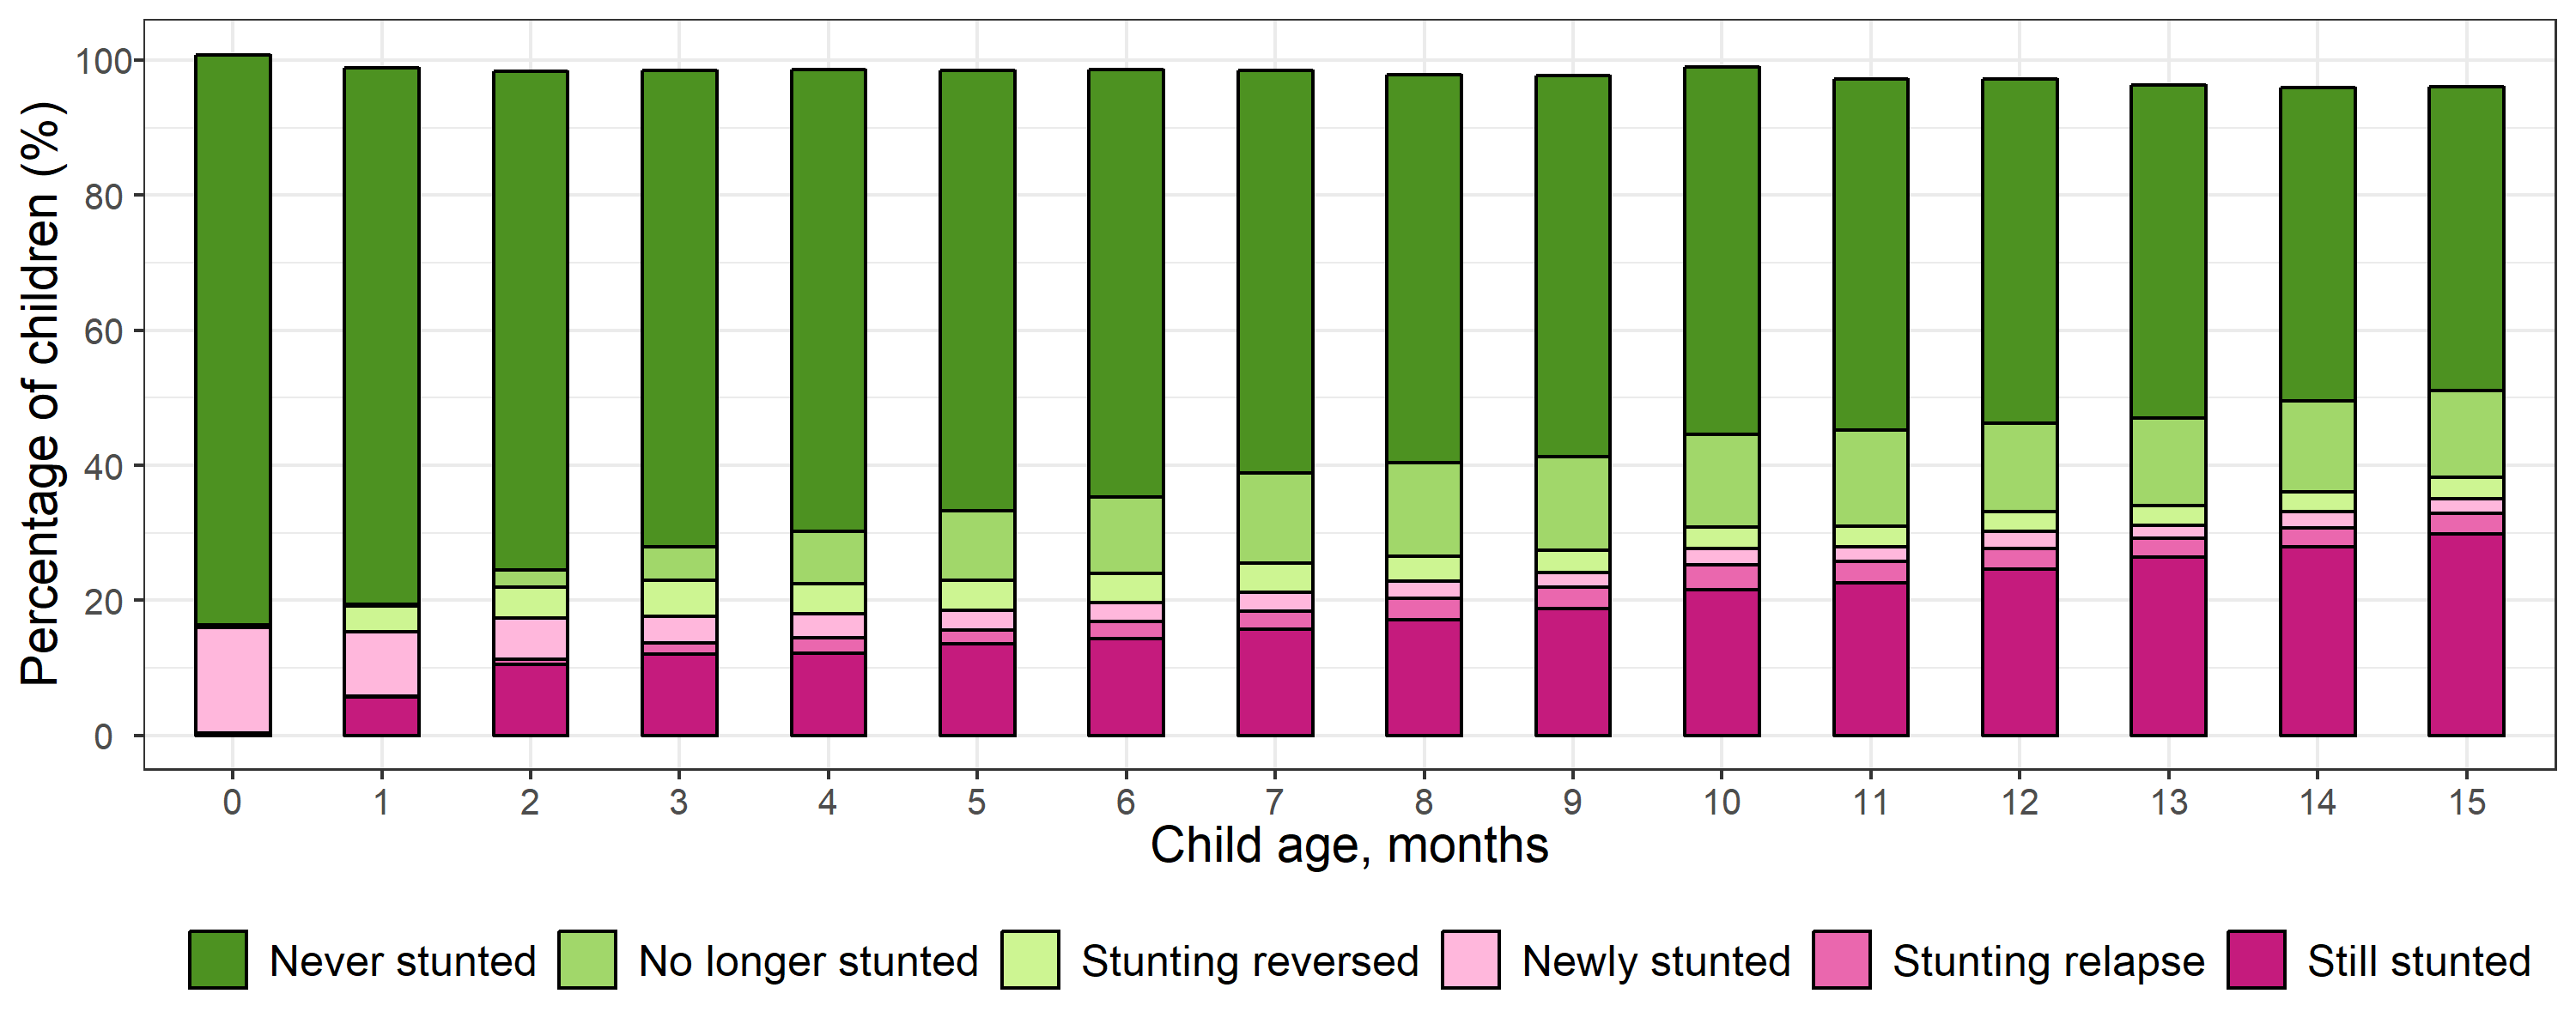
\includegraphics[width=41.67in]{C:/Users/andre/Documents/HBGDki/stunting/ki-longitudinal-manuscripts/figures/stunting/fig-stunt-2-flow-overall--allage-re}

\subsection{Fixed effects}\label{fixed-effects-2}

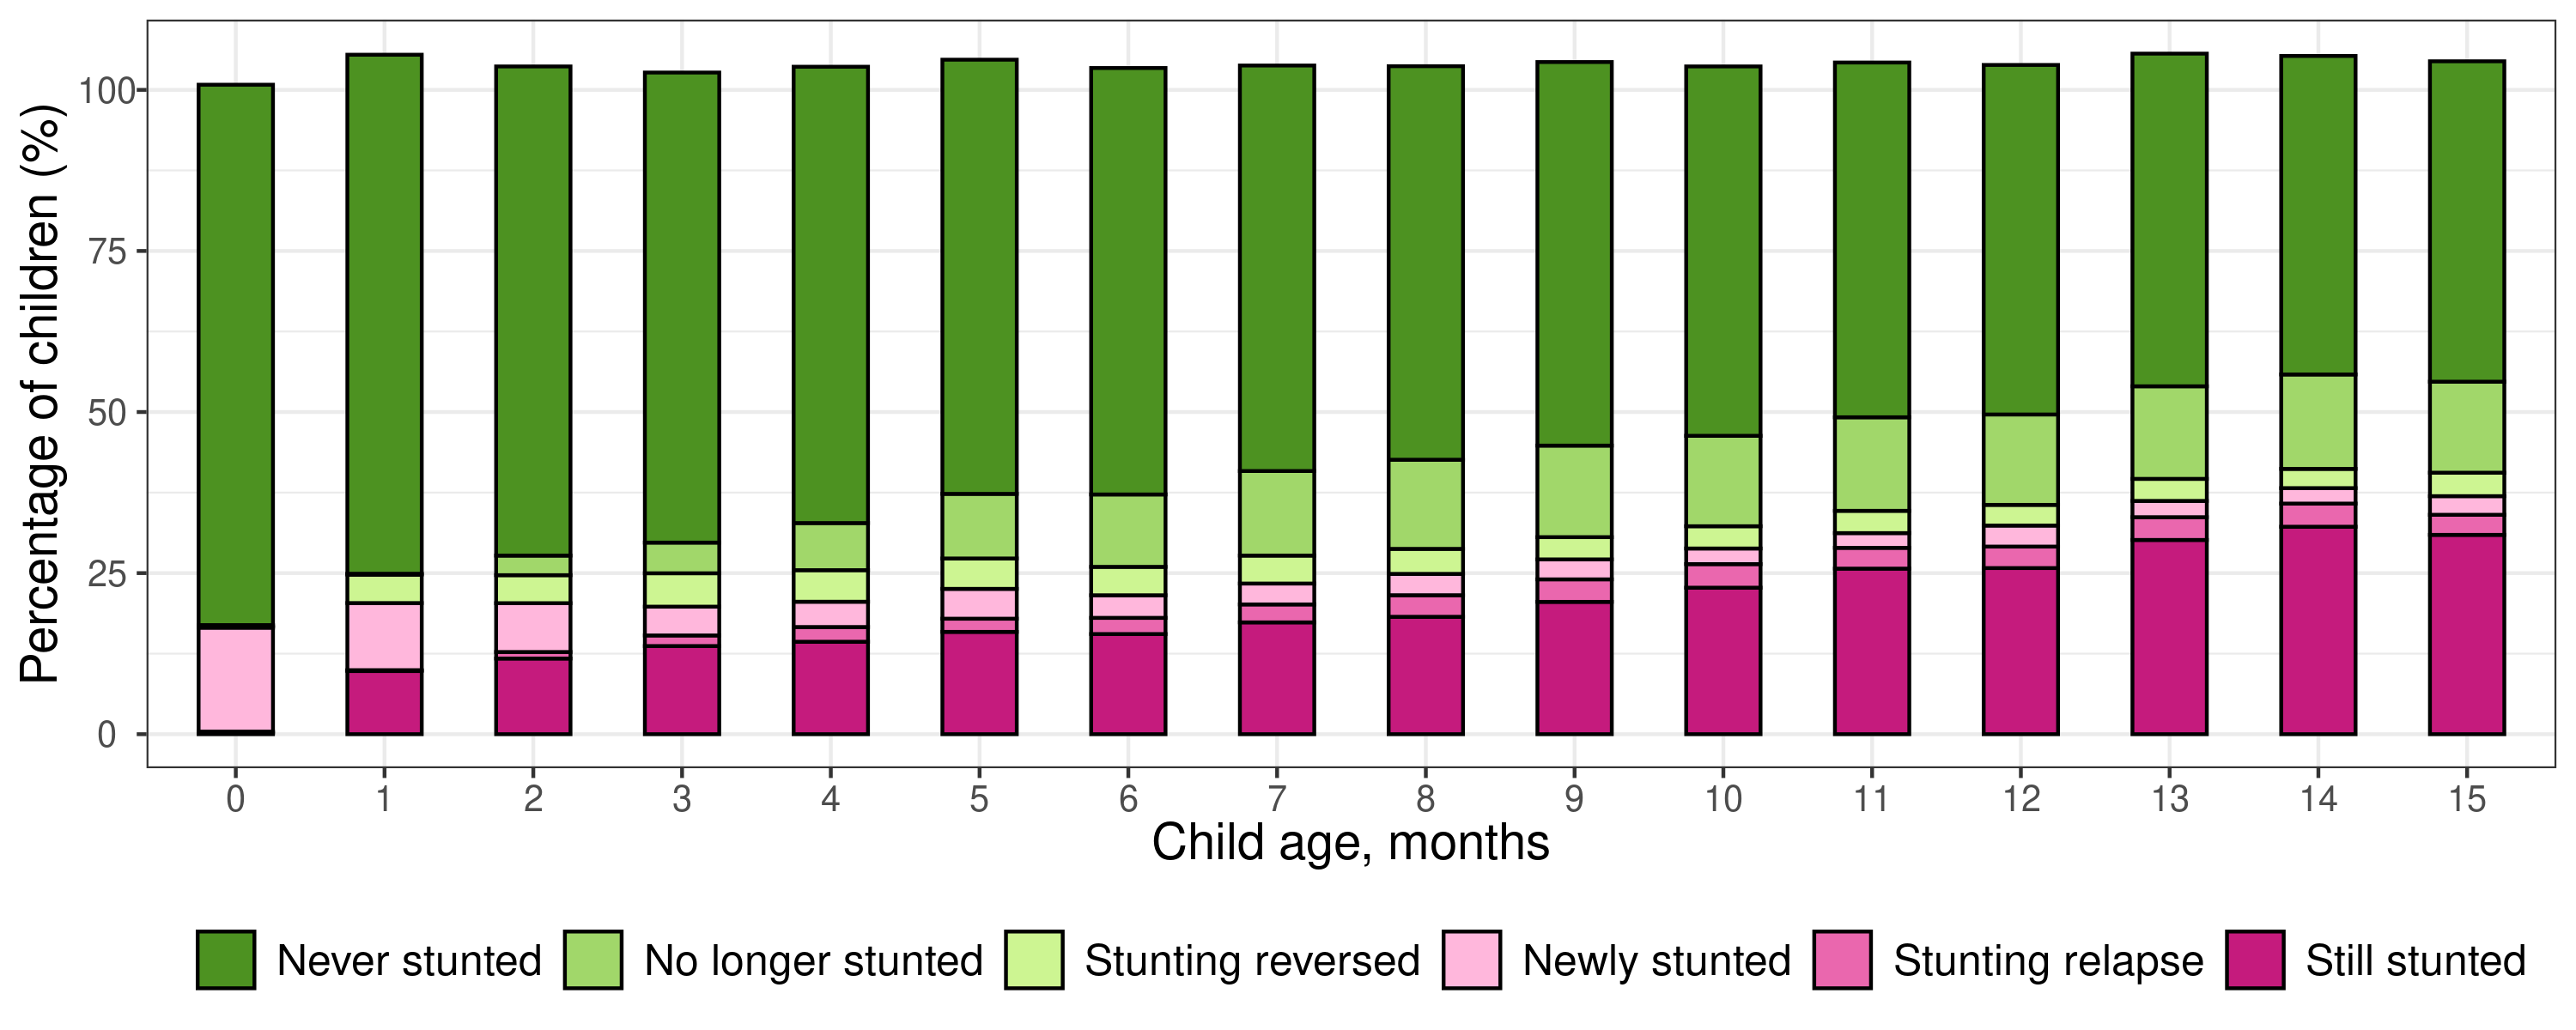
\includegraphics[width=41.67in]{C:/Users/andre/Documents/HBGDki/stunting/ki-longitudinal-manuscripts/figures/stunting/fig-stunt-2-flow-overall--allage-fe}

{[}ADD CAPTION{]}

\section{Linear growth velocity}\label{linear-growth-velocity-1}

\subsection{Random effects}\label{random-effects-3}

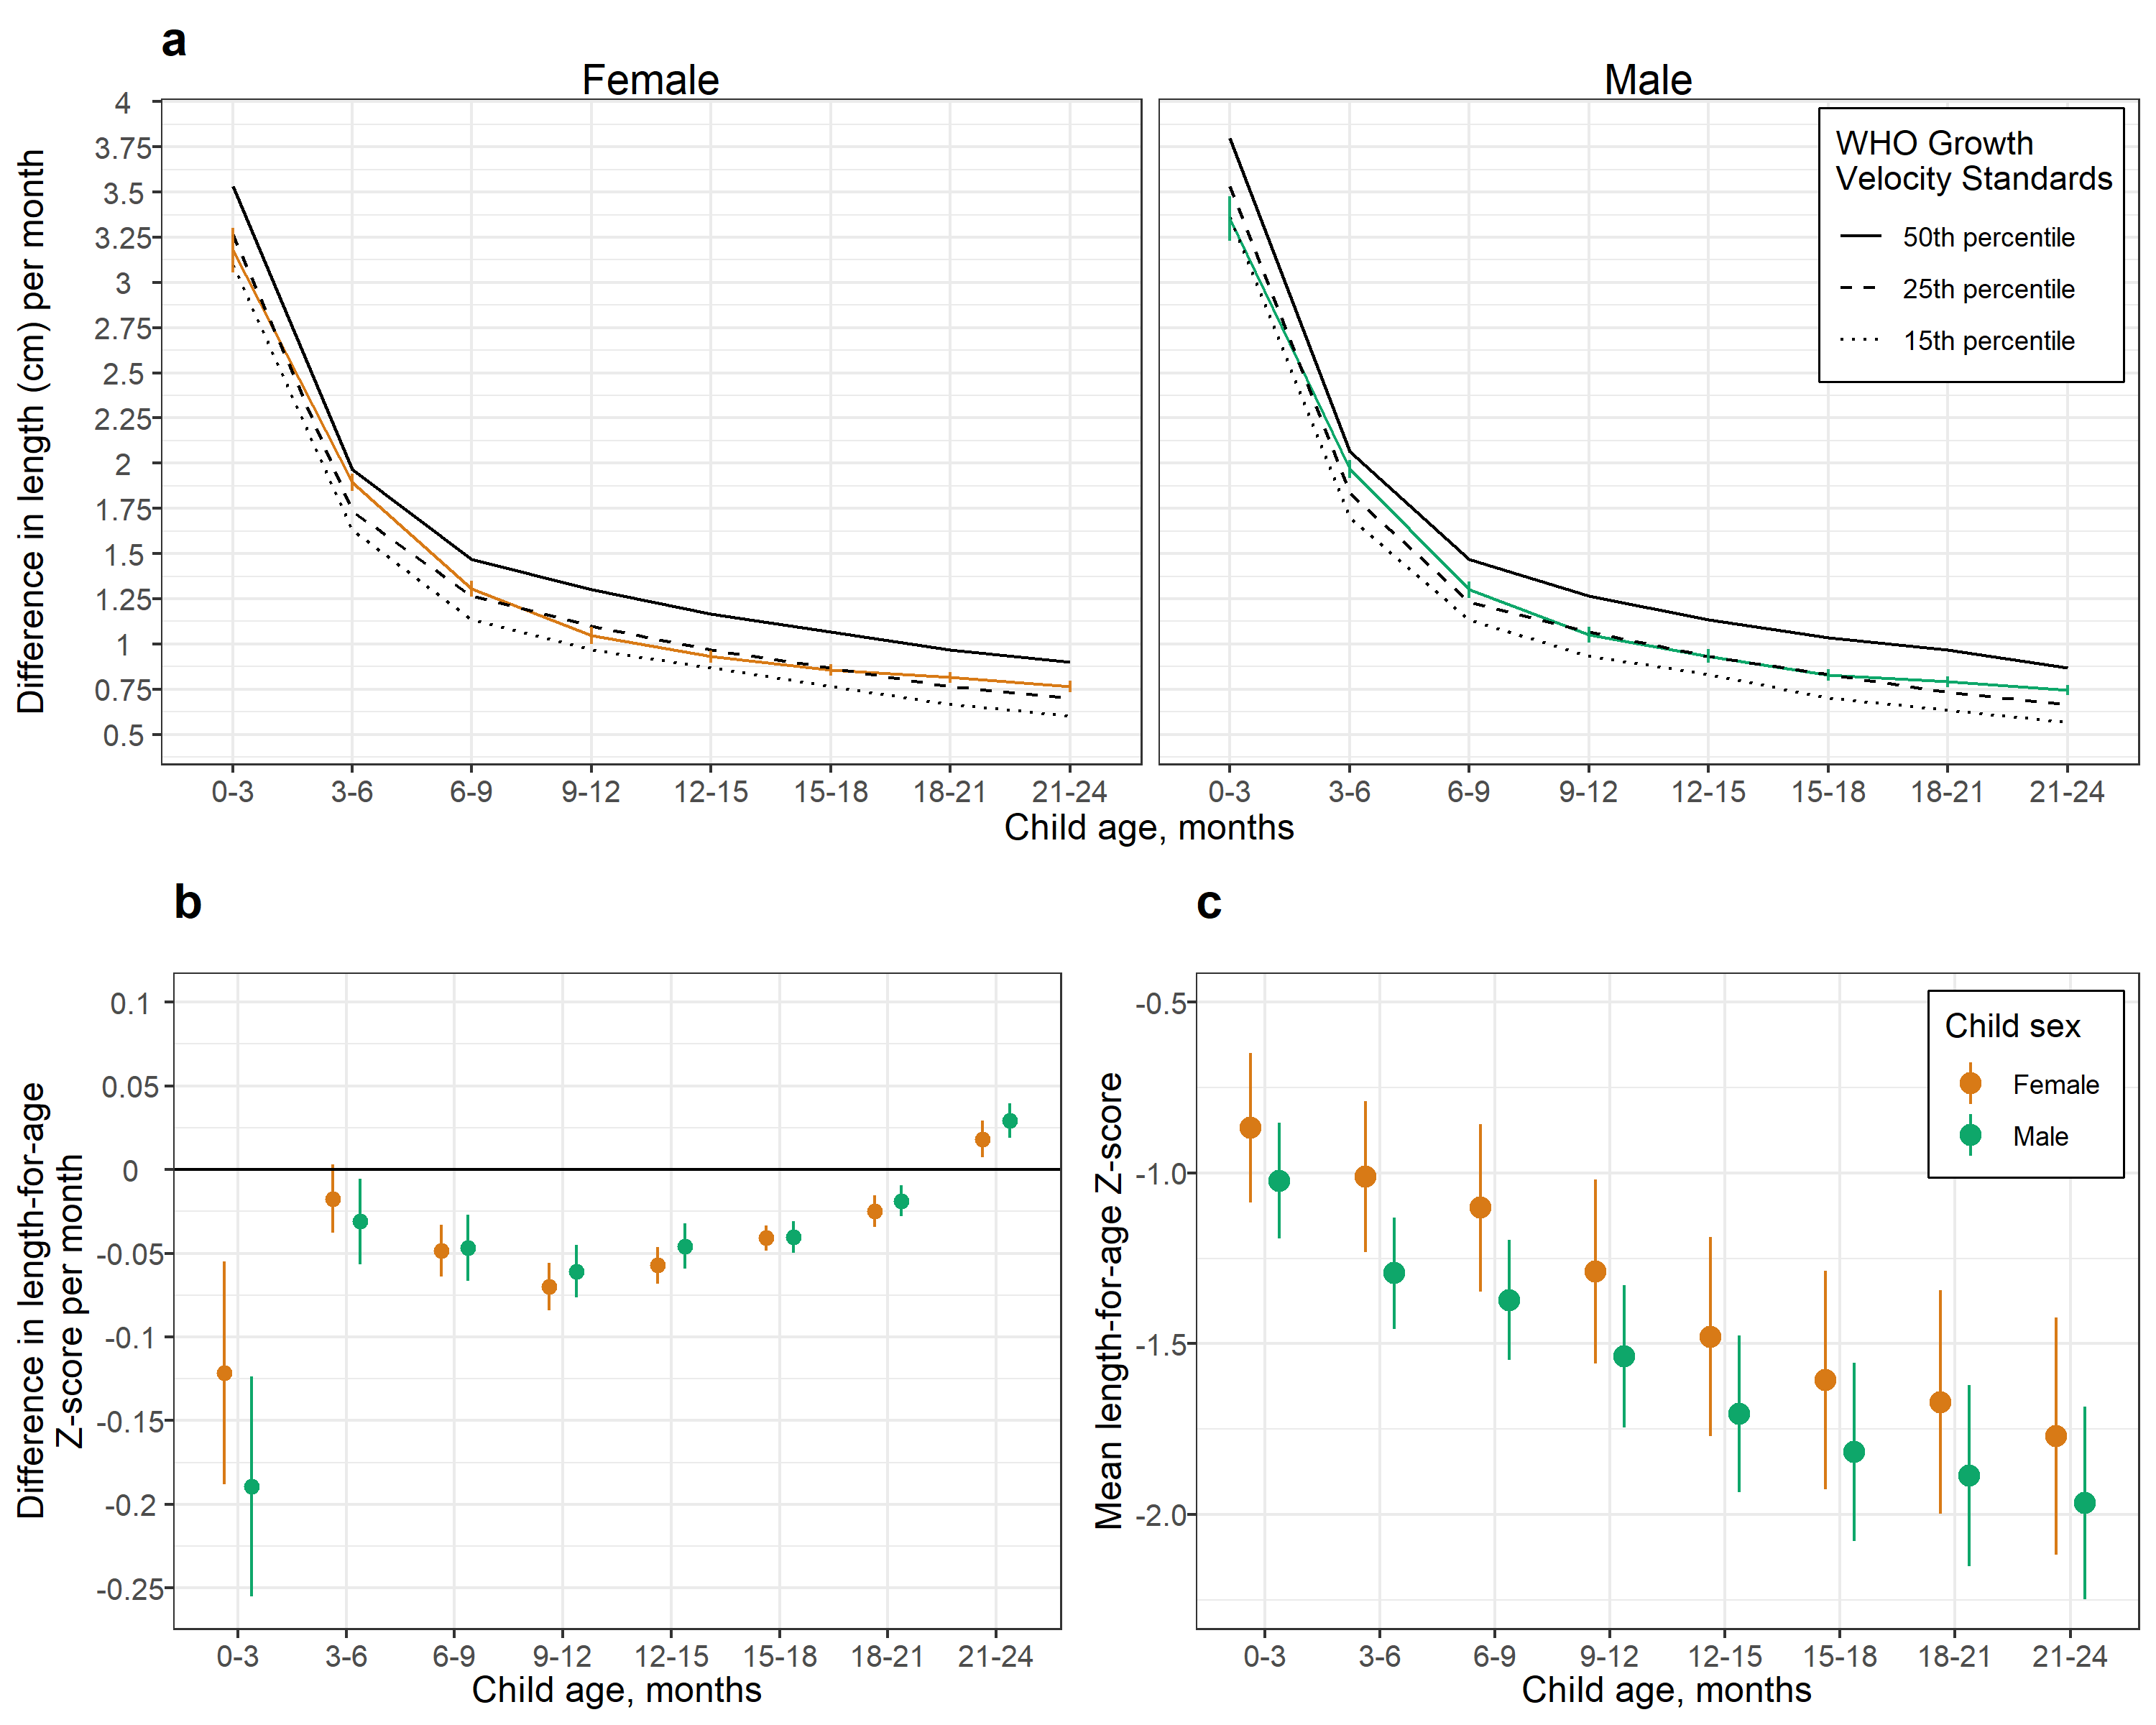
\includegraphics[width=41.67in]{C:/Users/andre/Documents/HBGDki/stunting/ki-longitudinal-manuscripts/figures/stunting/fig-stunt-2-vel-overall--allage-primary}

\subsection{Fixed effects}\label{fixed-effects-3}

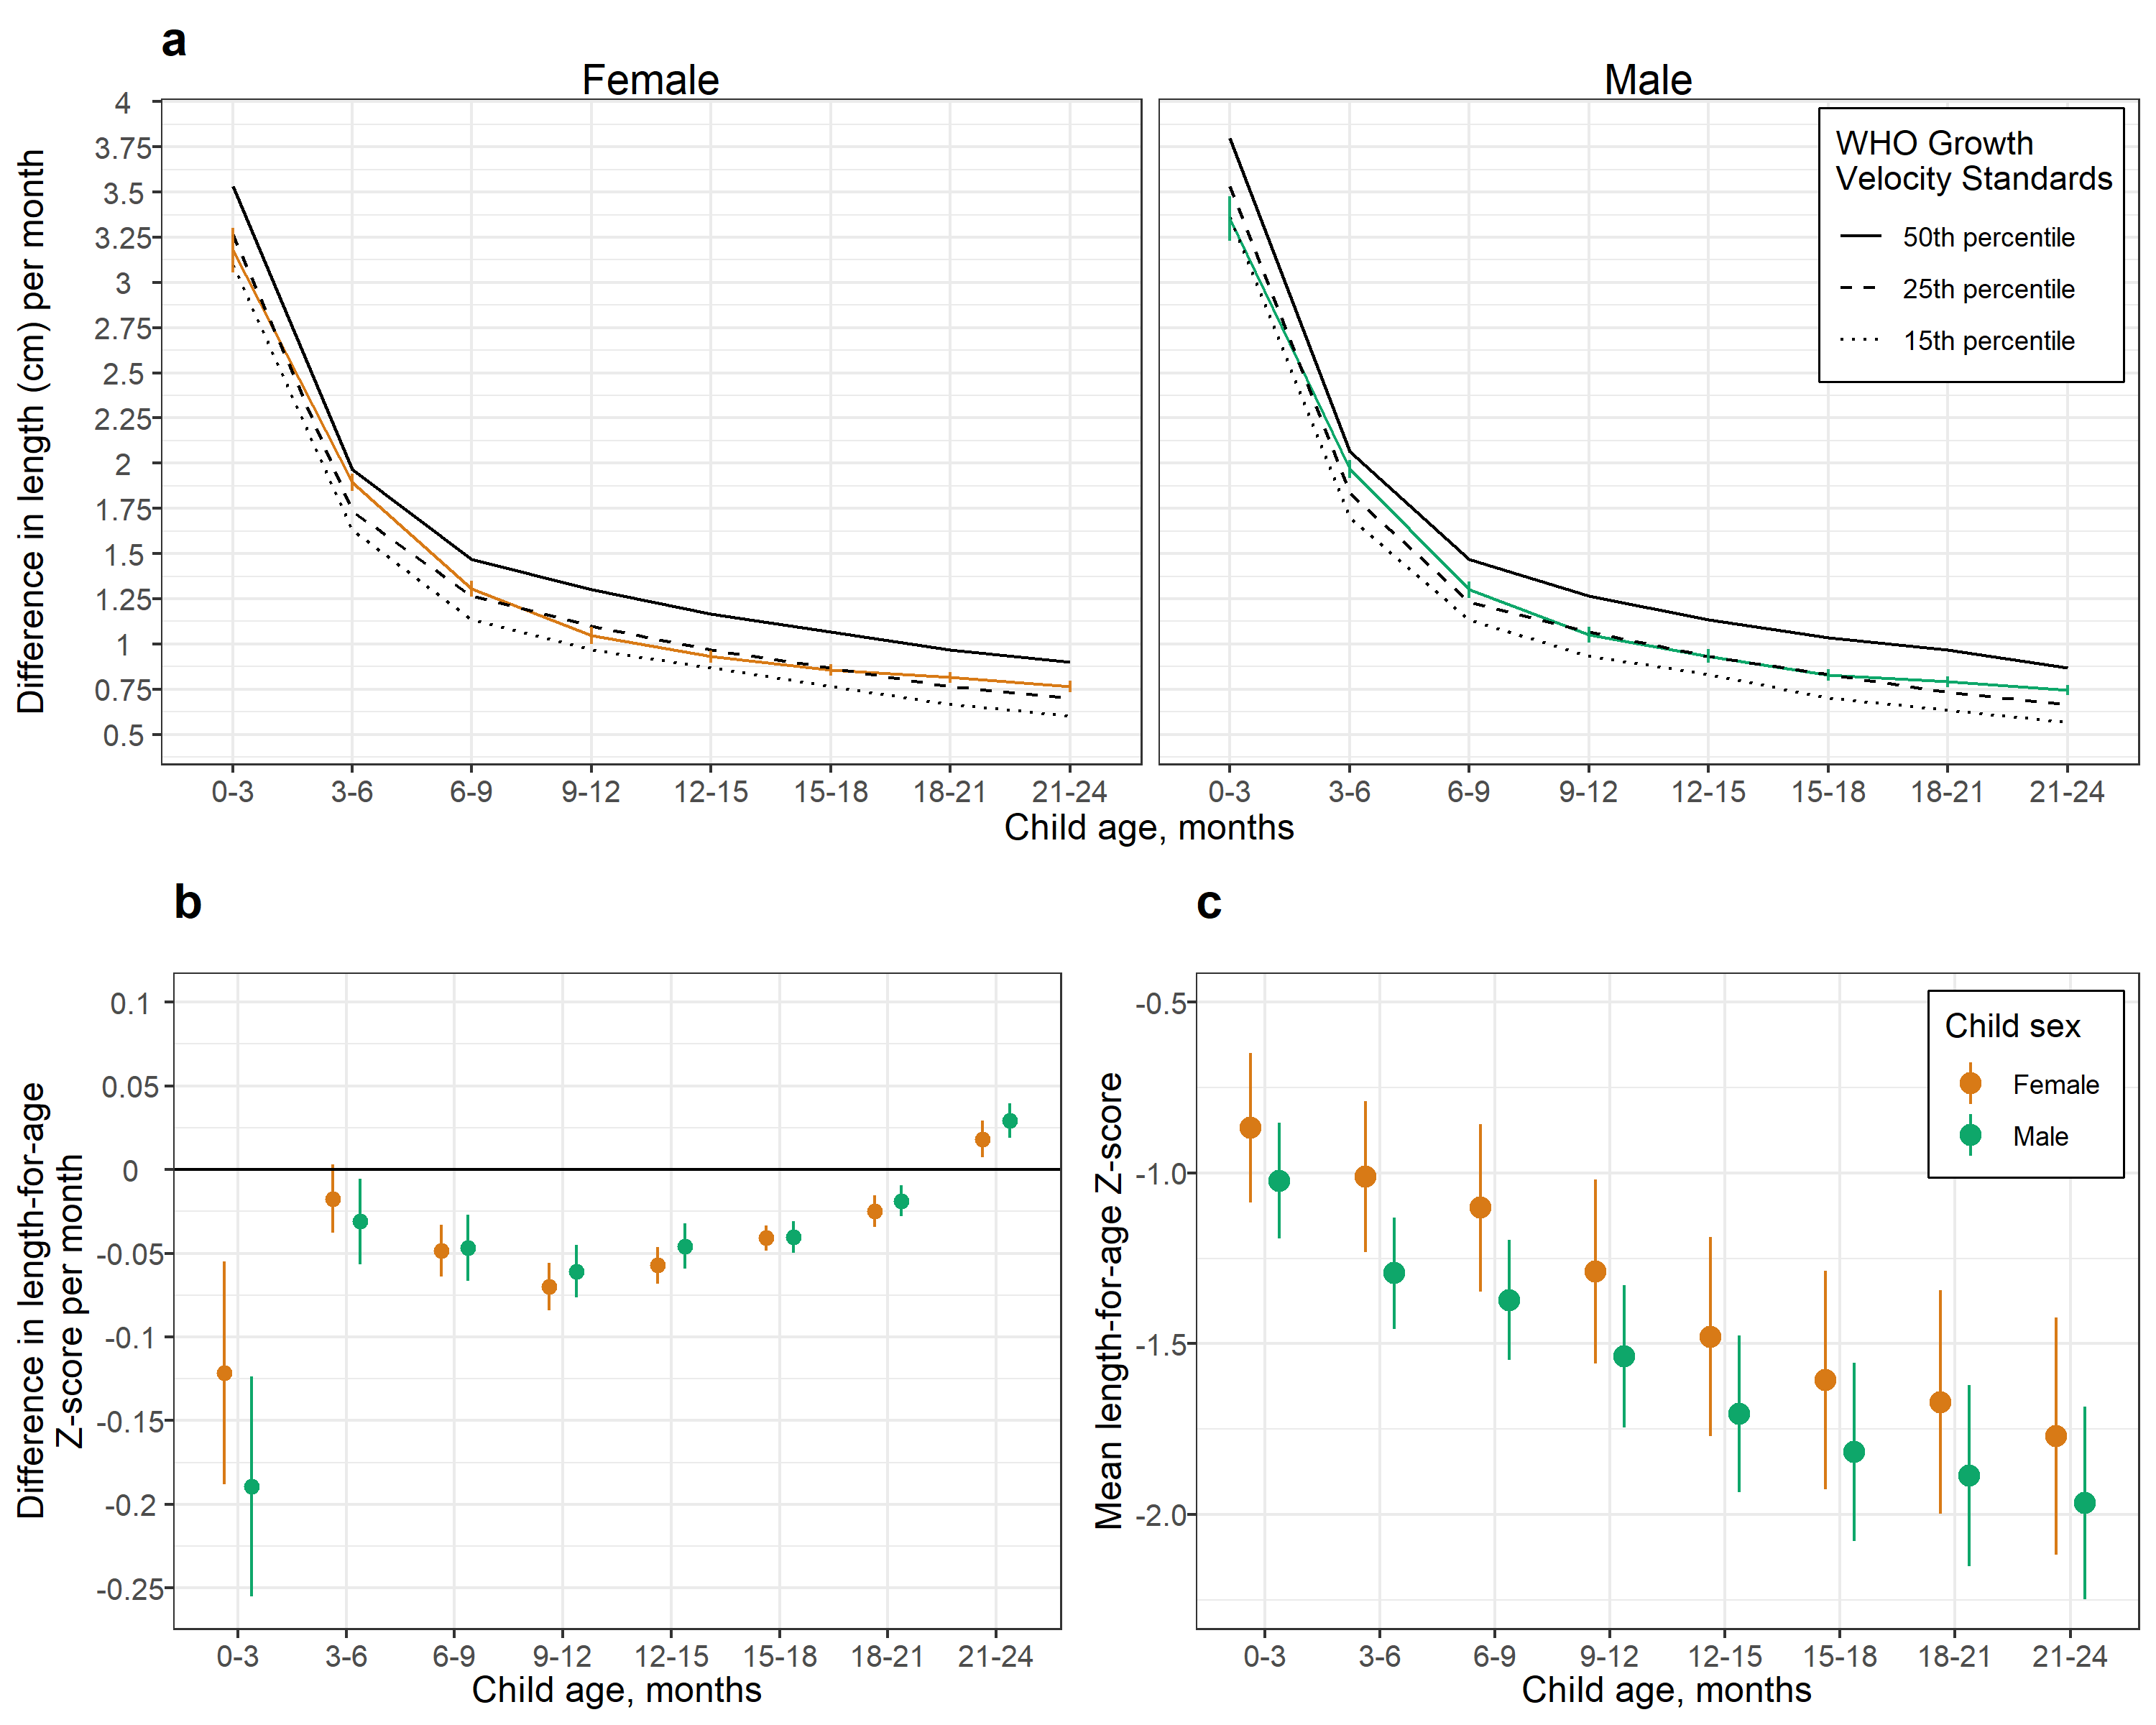
\includegraphics[width=41.67in]{C:/Users/andre/Documents/HBGDki/stunting/ki-longitudinal-manuscripts/figures/stunting/fig-stunt-2-vel-overall--allage-primary}

{[}ADD CAPTION{]}

\bibliography{book.bib,packages.bib}


\end{document}
